% \chapter{Appendix I}
% \label{sec:appendix}
% \blindtext[3]
%
% \chapter{Appendix II}
% \label{sec:appendix2}
% \blindtext[3]

\chapter{Appendix Validating RAPL Accuracy}
\label{app:validating_rapl_accuracy}
This section includes the plots for the correlation of the external reference measurent against individual RAPL metrics as described in ~\secref{validating_rapl_accuracy}.

\begin{figure}[]
    \centering
    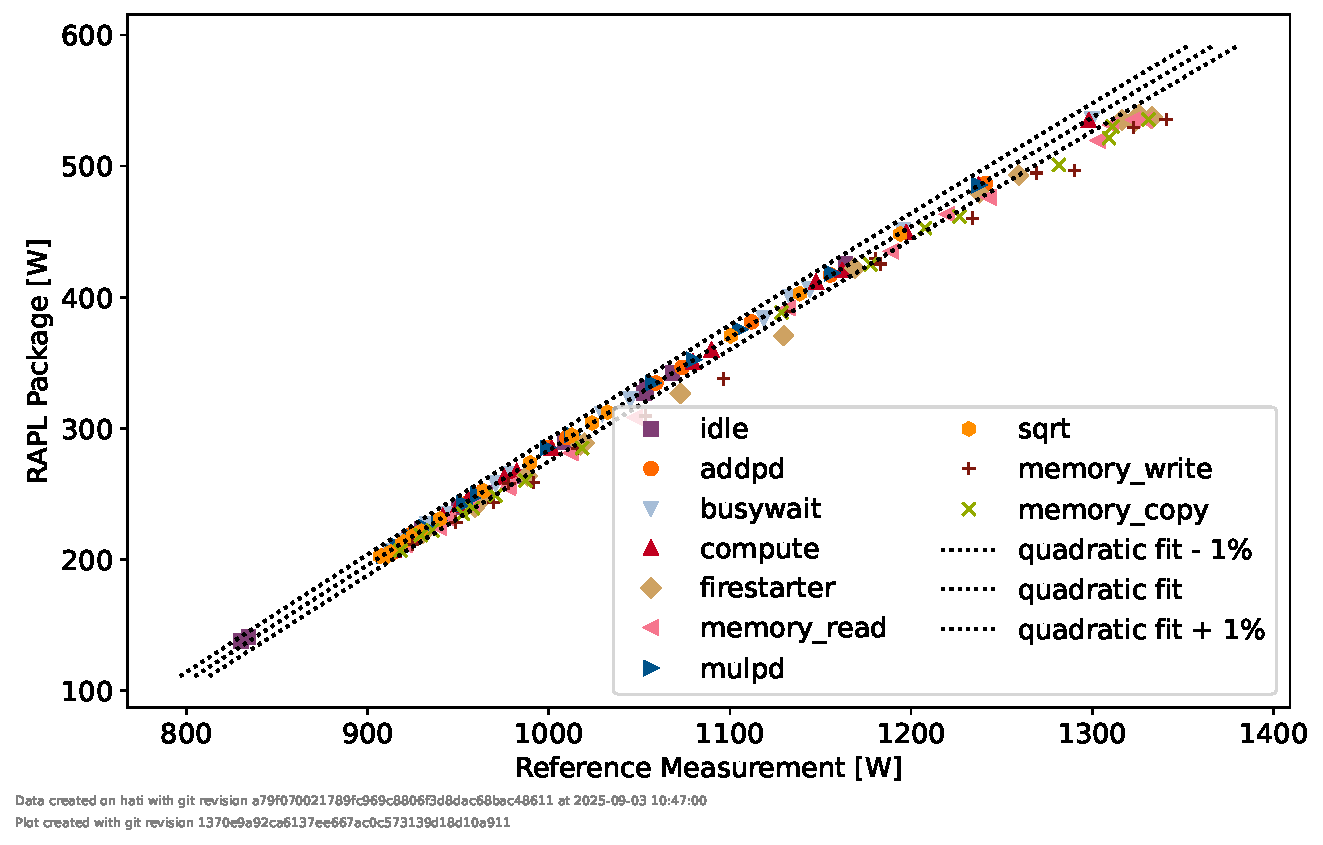
\includegraphics[width=0.8\columnwidth]{fig/rapl-accuracy/rapl-accuracy-package.pdf}
    \caption{The roco2 microbenchmark is executed on a varying number of cores with different frequencies.
    The RAPL package measurement is mapped with a quadratic fit to the external reference measurement for compute kernels which do no access the DRAM.}
\end{figure}

\begin{figure}[]
    \centering
    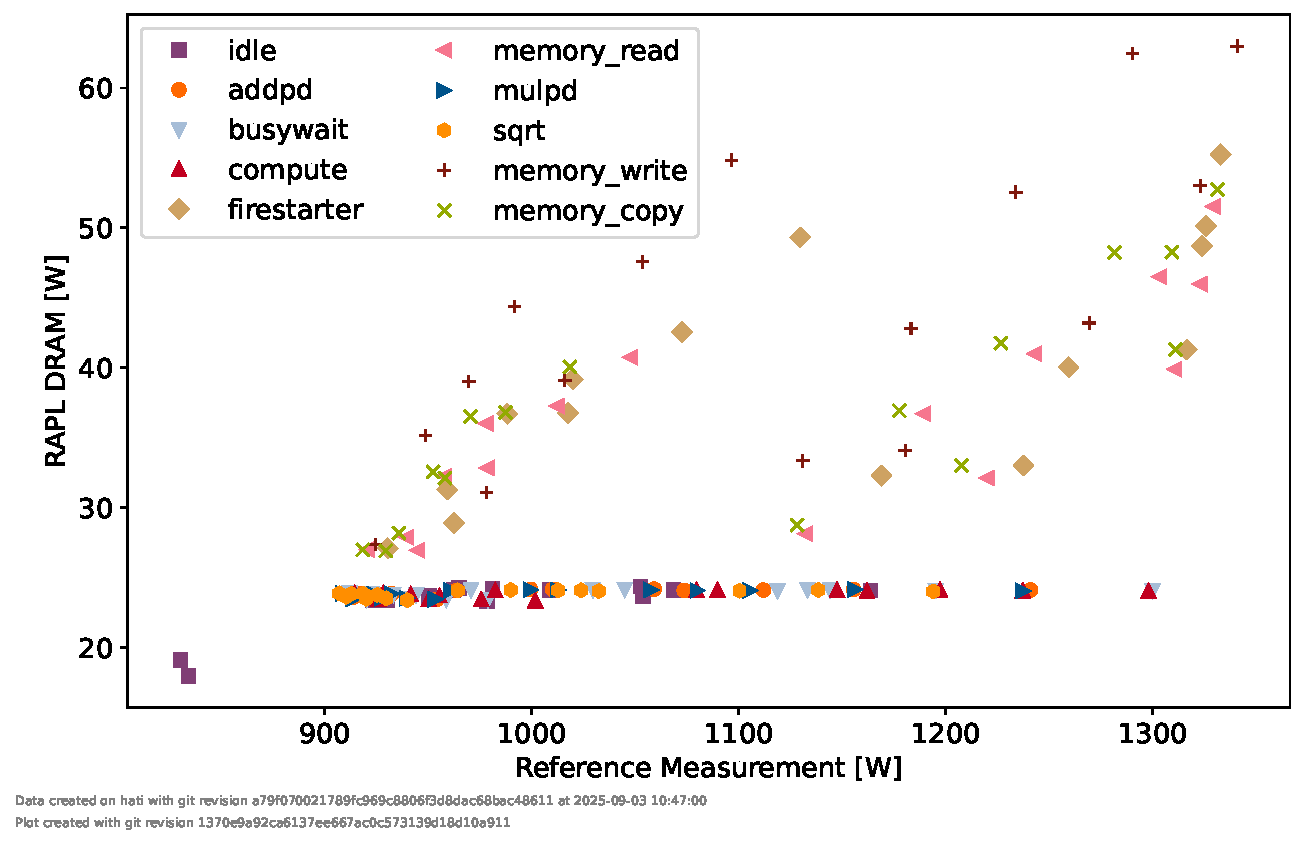
\includegraphics[width=0.8\columnwidth]{fig/rapl-accuracy/rapl-accuracy-dram.pdf}
    \caption{The roco2 microbenchmark is executed on a varying number of cores with different frequencies.}
\end{figure}

\chapter{Appendix P-State Latencies}
\label{app:pstate_latencies_scatter_complete}
This section includes the scatter plots for all measurement points from the ftalat benchmark as described in~\secref{pstate_latencies}.

\begin{figure}[]
    \centering
    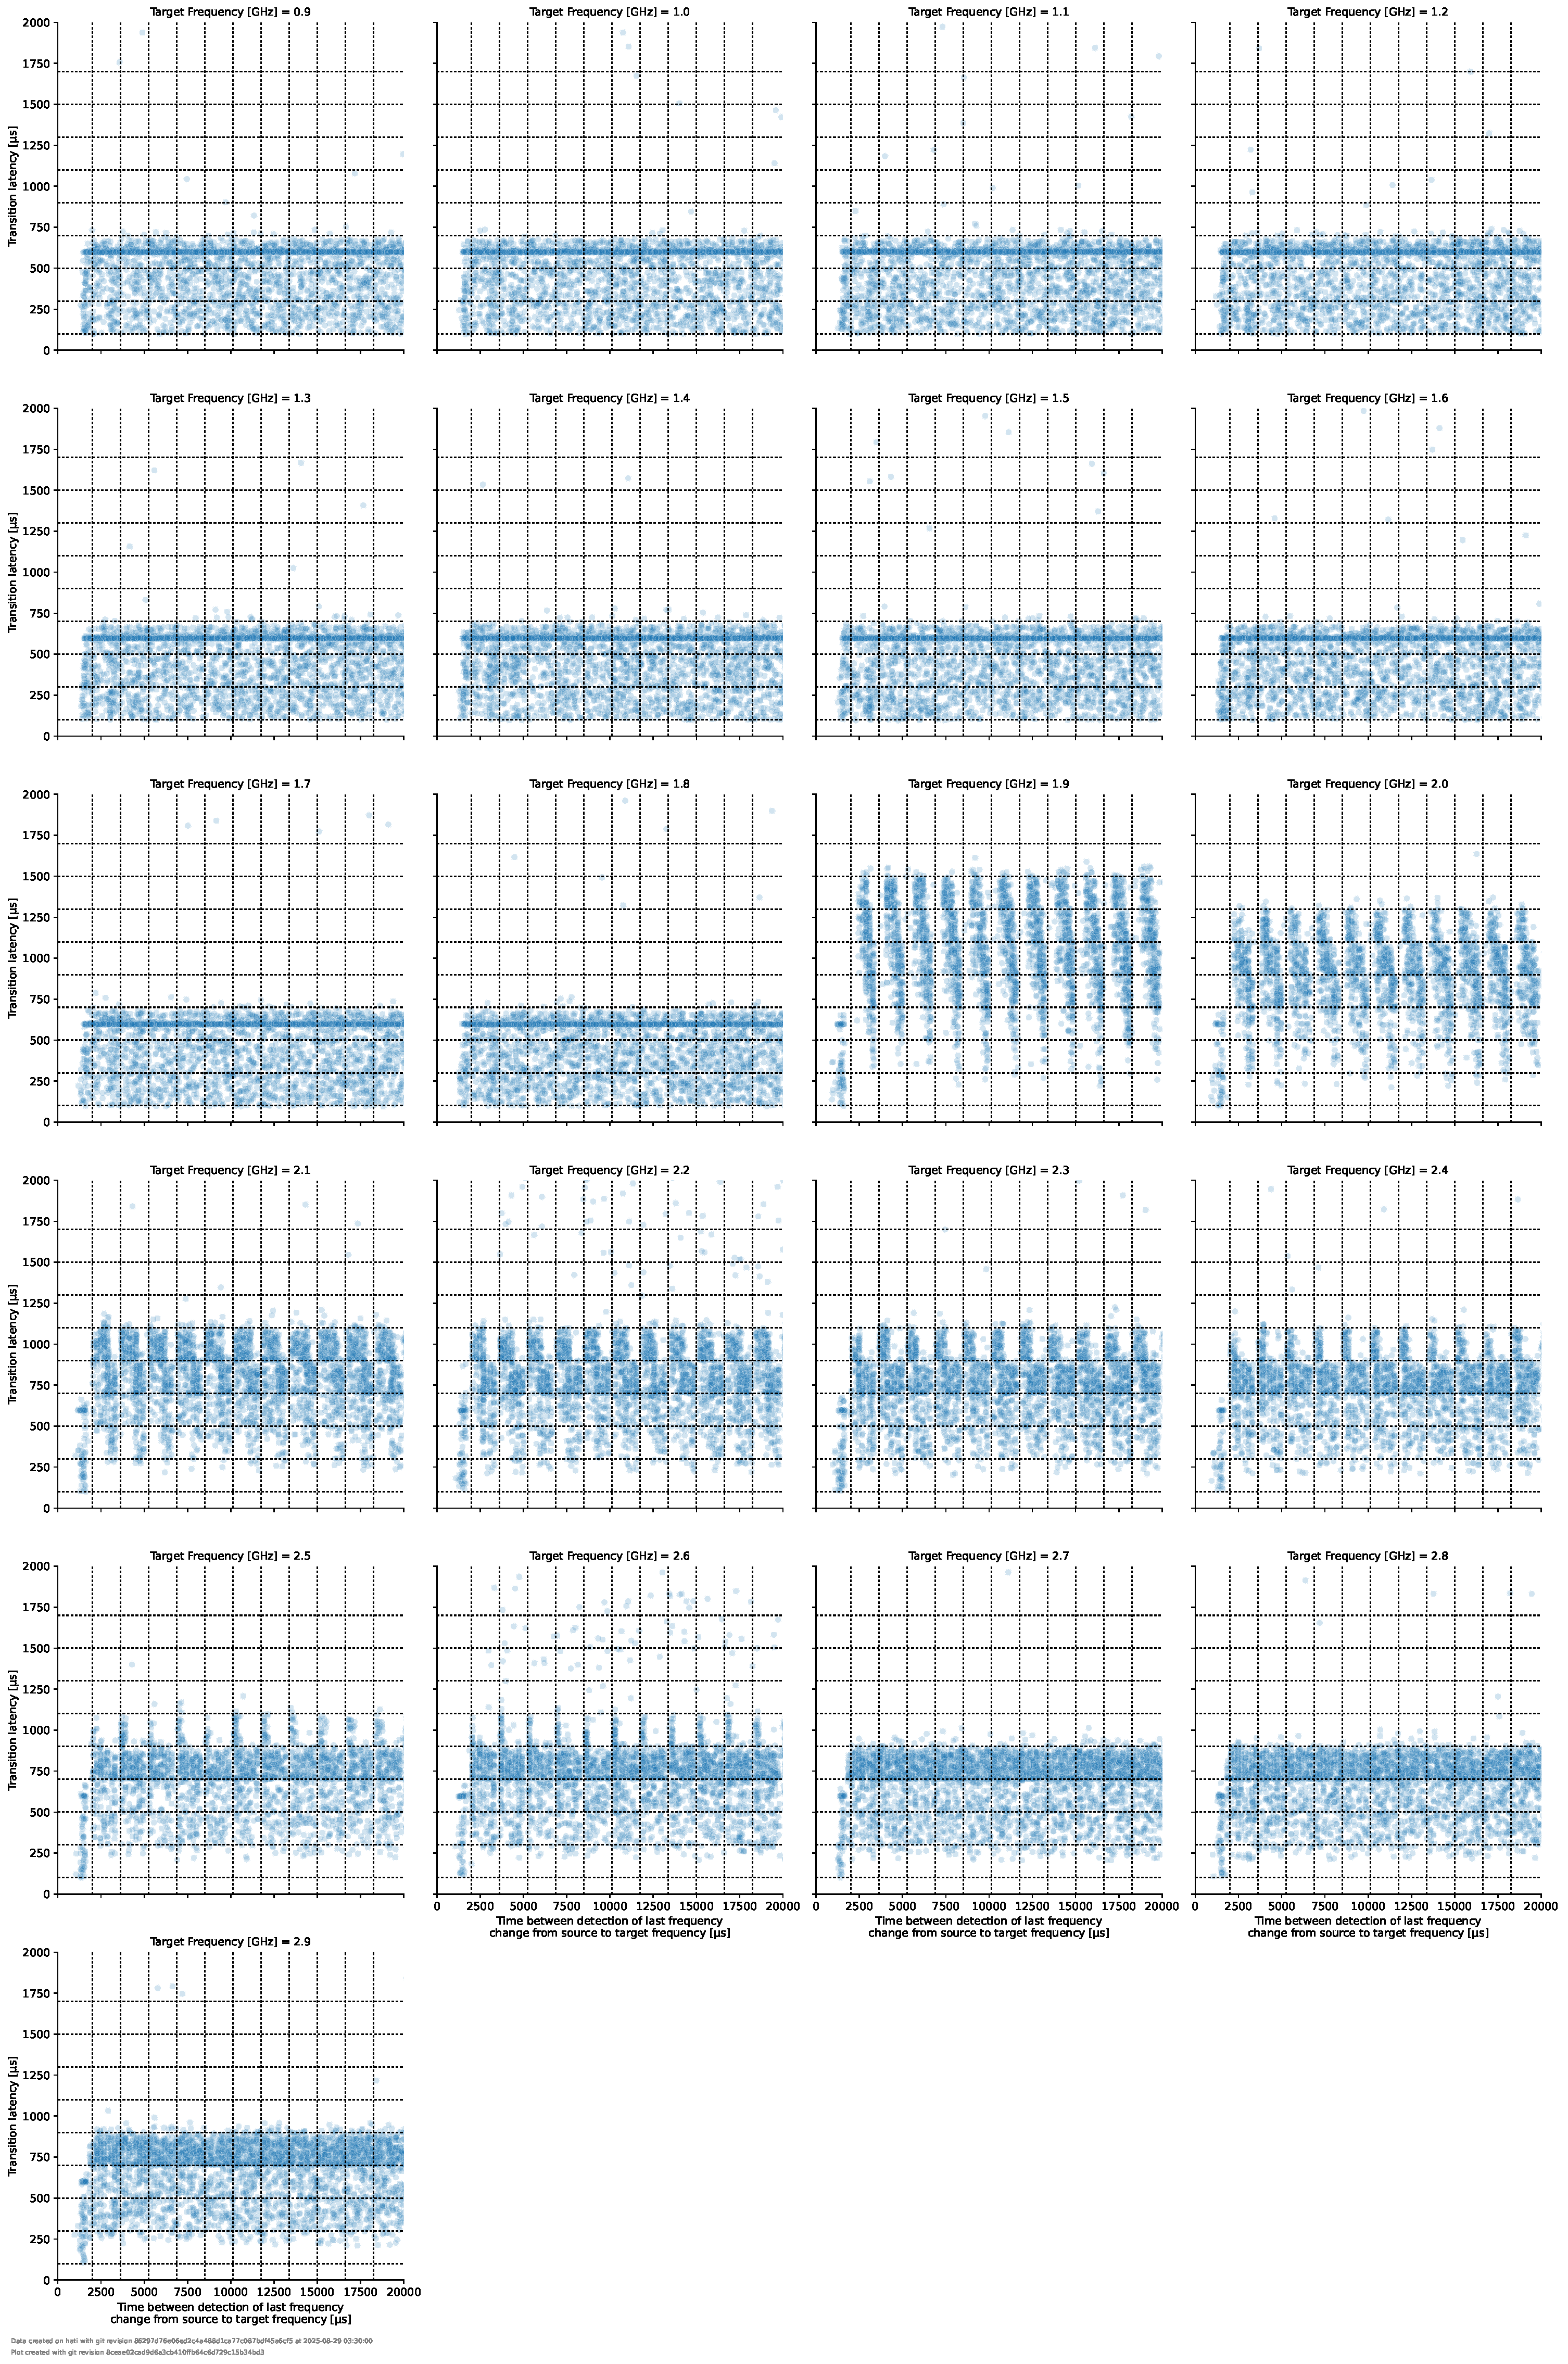
\includegraphics[width=\columnwidth]{fig/ftalat/ftalat_scatter_wait_transition_latency_hati_source_0.8.pdf}
    \caption{Dependance of the time between the detection events of transitions from \SI{0.8}{\GHz} to \SI{0.9}{}, \SI{1.0}{}, ..., \SI{2.9}{\GHz}. For better lines for bins of size \SI{1625}{\us} and \SI{200}{\us} have been included for the x and y-axis respectively.}
\end{figure}
\begin{figure}[]
    \centering
    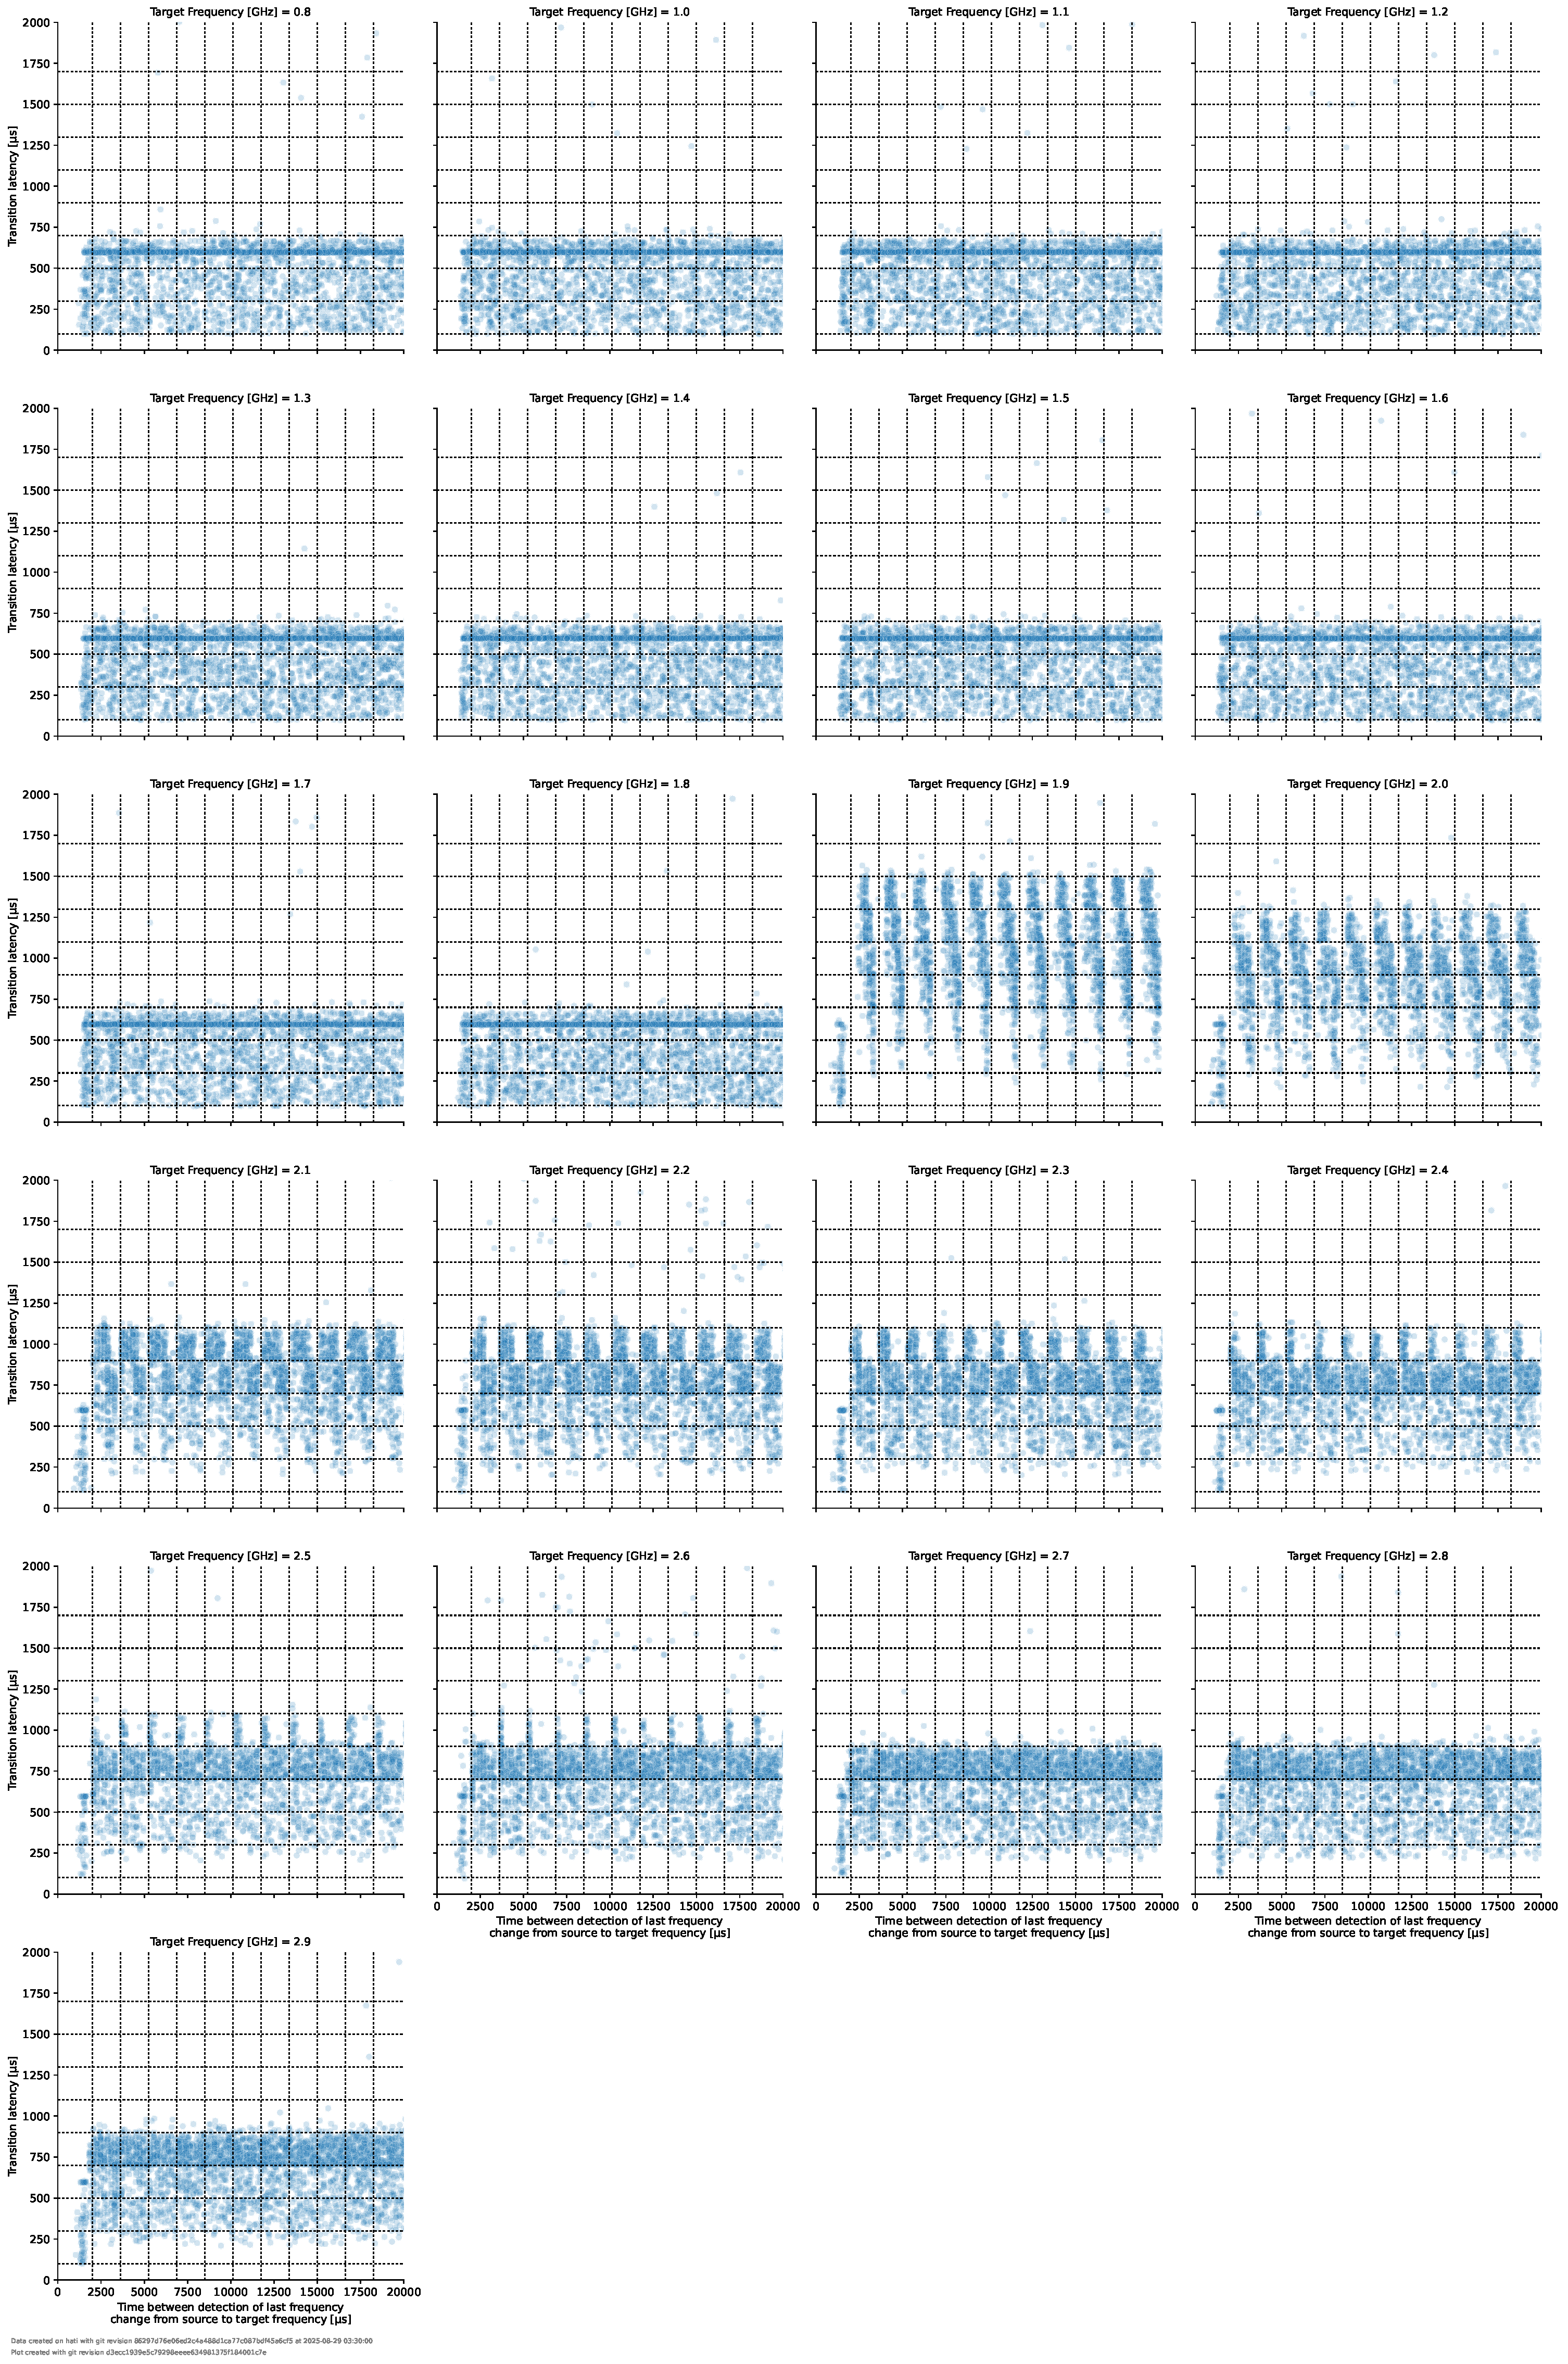
\includegraphics[width=\columnwidth]{fig/ftalat/ftalat_scatter_wait_transition_latency_hati_source_0.9.pdf}
    \caption{Dependance of the time between the detection events of transitions from \SI{0.9}{\GHz} to \SI{0.8}{}, \SI{1.0}{}, ..., \SI{2.9}{\GHz}. For better lines for bins of size \SI{1625}{\us} and \SI{200}{\us} have been included for the x and y-axis respectively.}
\end{figure}
\begin{figure}[]
    \centering
    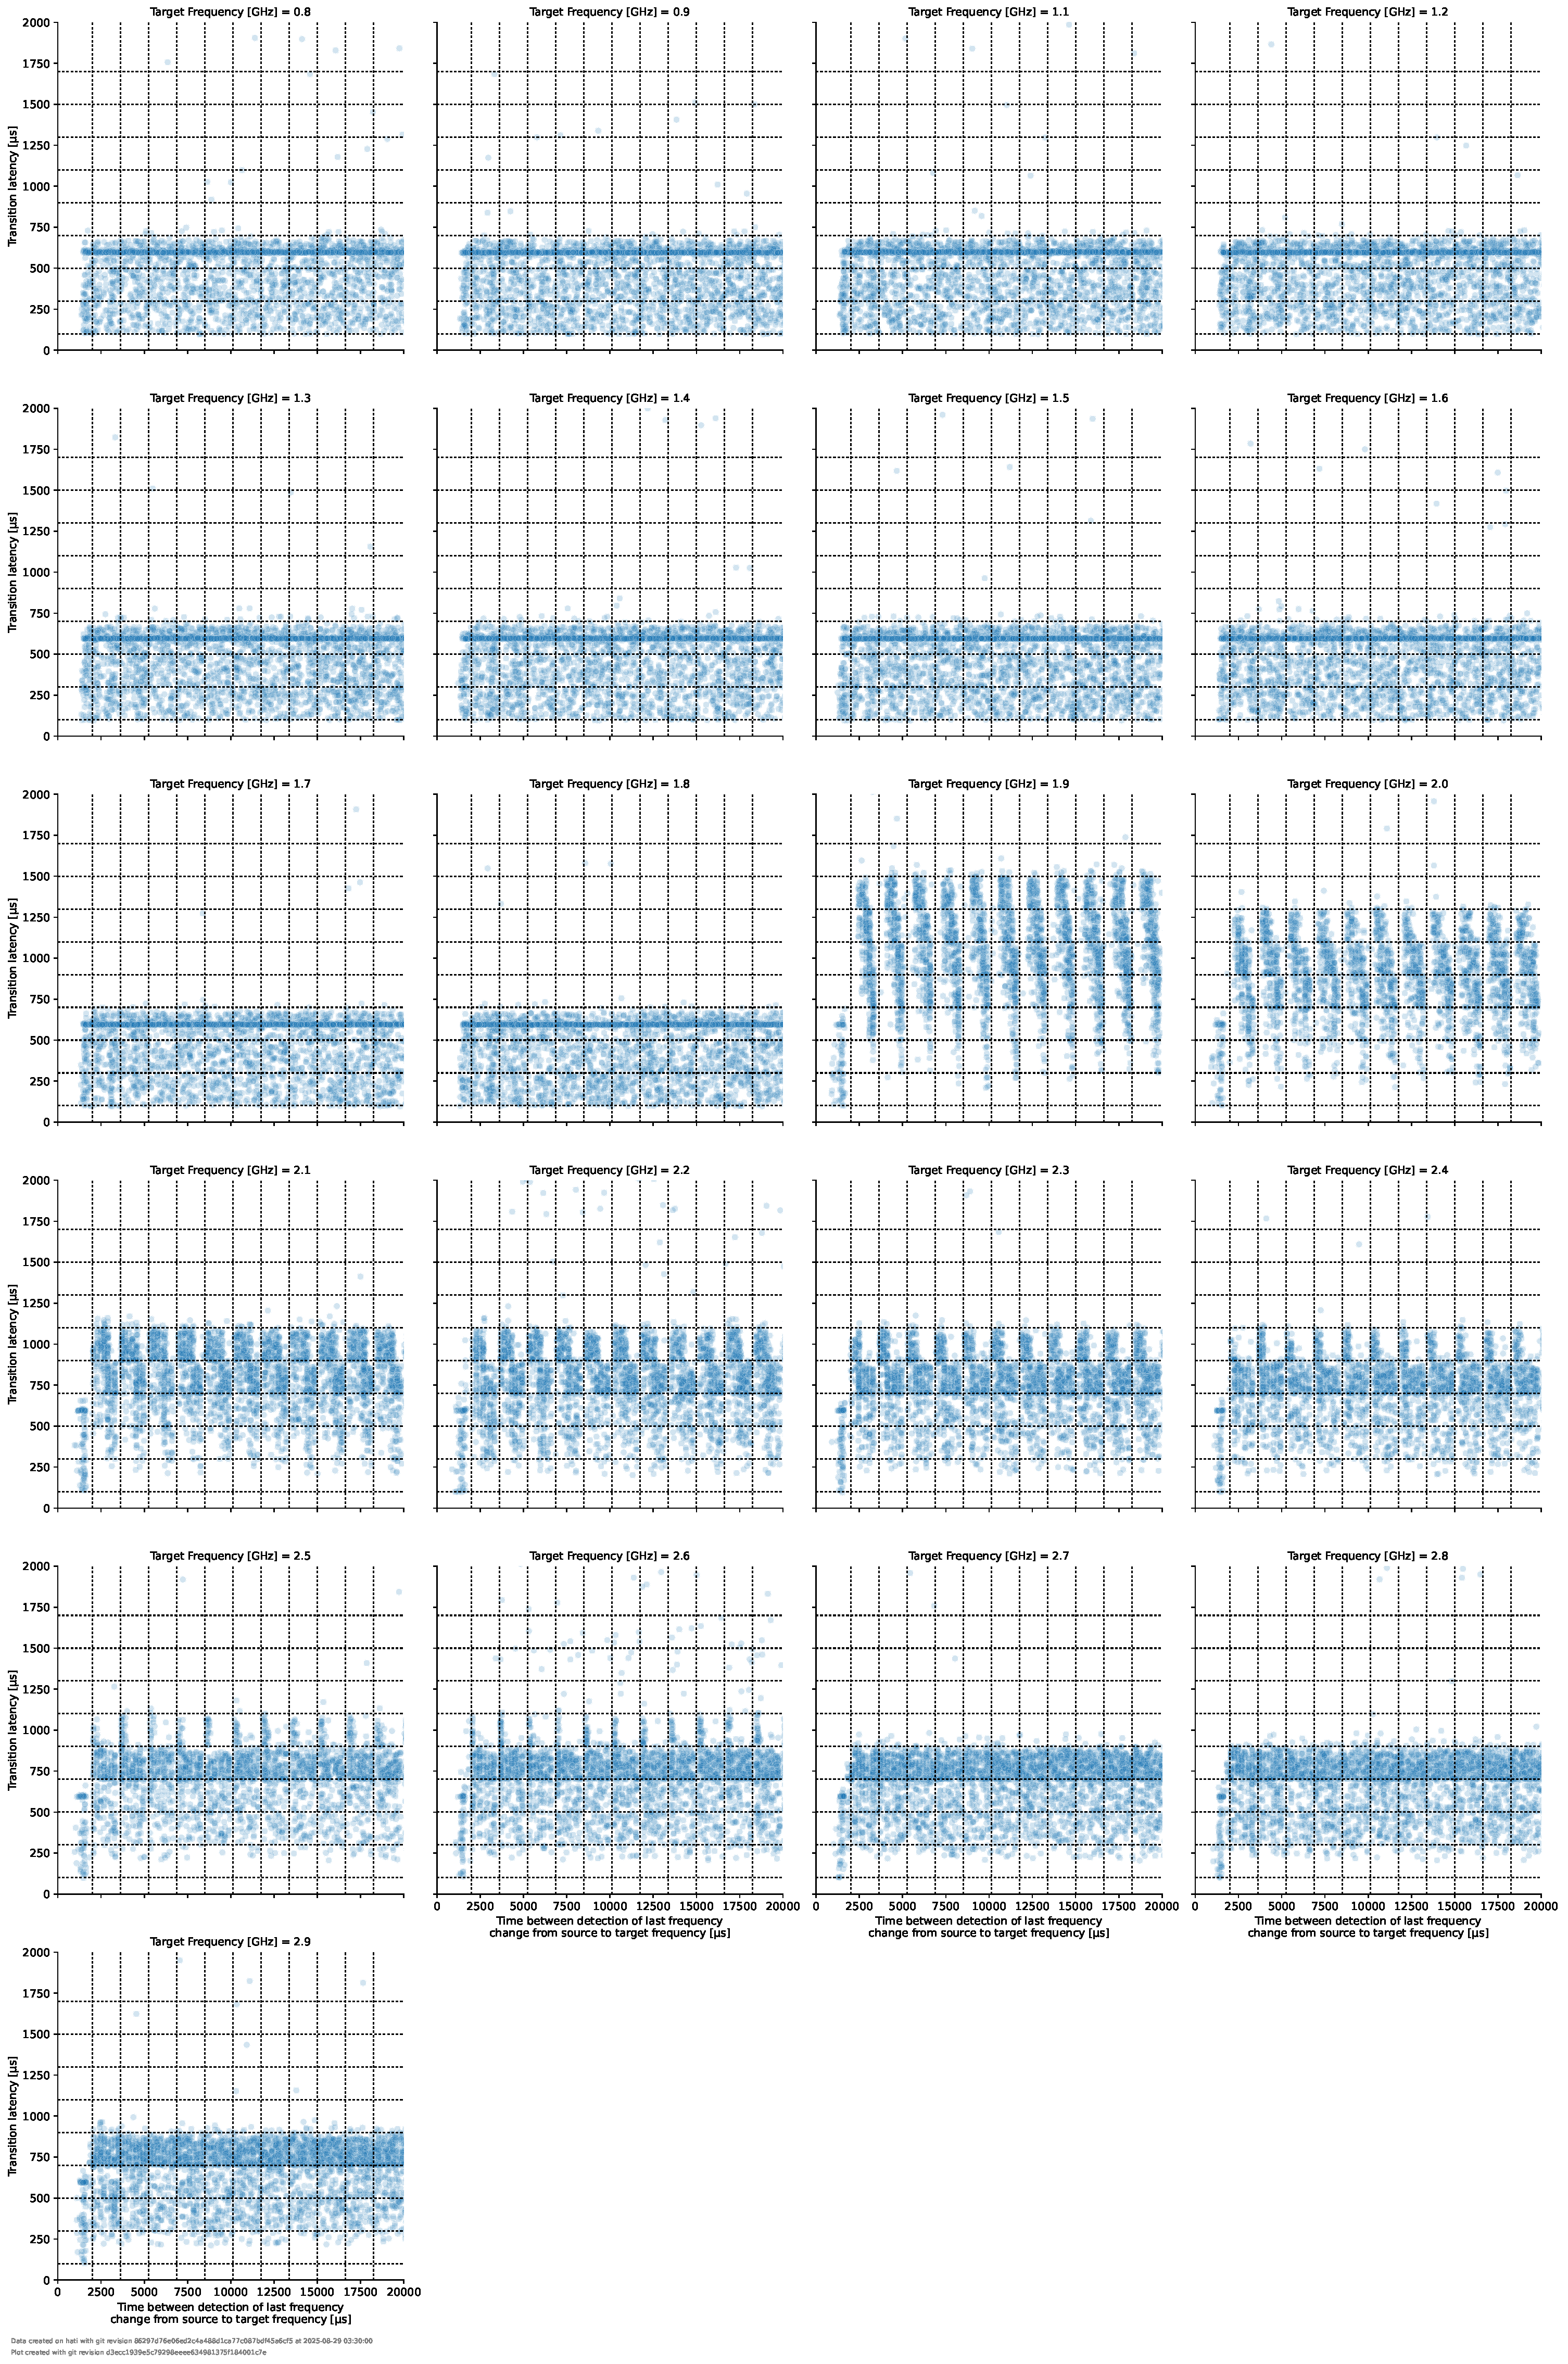
\includegraphics[width=\columnwidth]{fig/ftalat/ftalat_scatter_wait_transition_latency_hati_source_1.0.pdf}
    \caption{Dependance of the time between the detection events of transitions from \SI{1.0}{\GHz} to \SI{0.8}{}, \SI{0.9}{}, ..., \SI{2.9}{\GHz}. For better lines for bins of size \SI{1625}{\us} and \SI{200}{\us} have been included for the x and y-axis respectively.}
\end{figure}
\begin{figure}[]
    \centering
    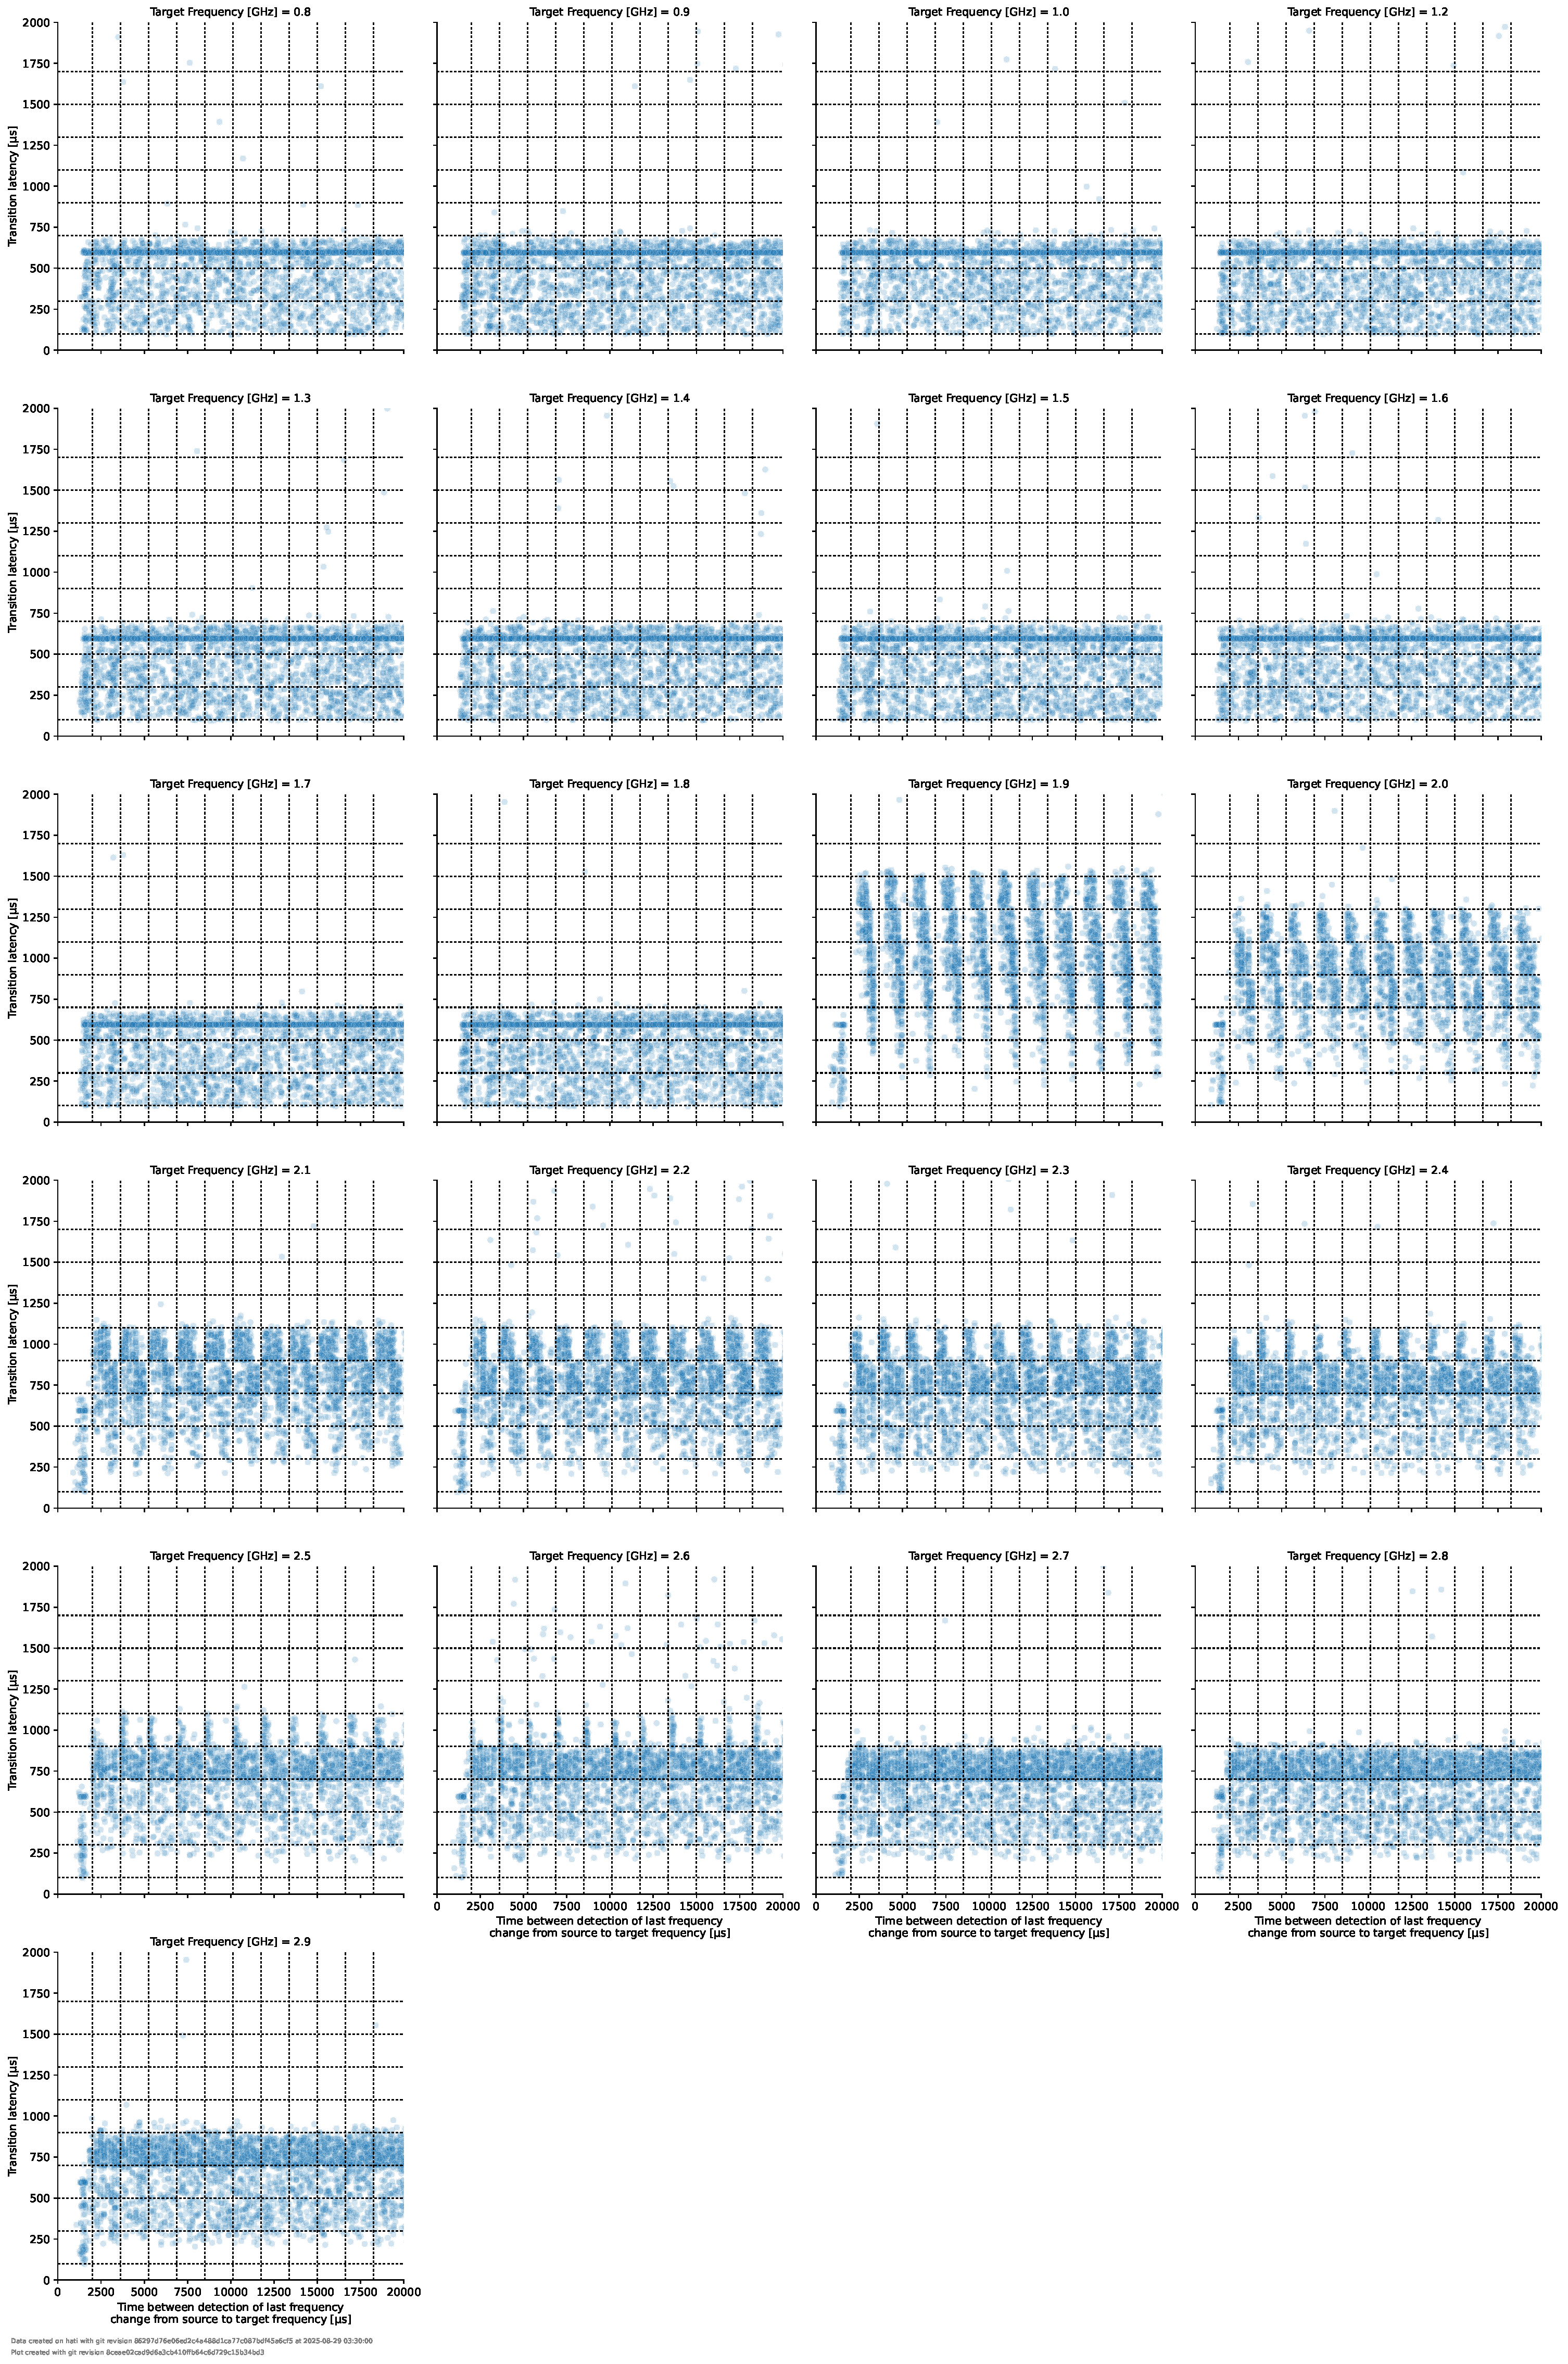
\includegraphics[width=\columnwidth]{fig/ftalat/ftalat_scatter_wait_transition_latency_hati_source_1.1.pdf}
    \caption{Dependance of the time between the detection events of transitions from \SI{1.1}{\GHz} to \SI{0.8}{}, \SI{0.9}{}, ..., \SI{2.9}{\GHz}. For better lines for bins of size \SI{1625}{\us} and \SI{200}{\us} have been included for the x and y-axis respectively.}
\end{figure}
\begin{figure}[]
    \centering
    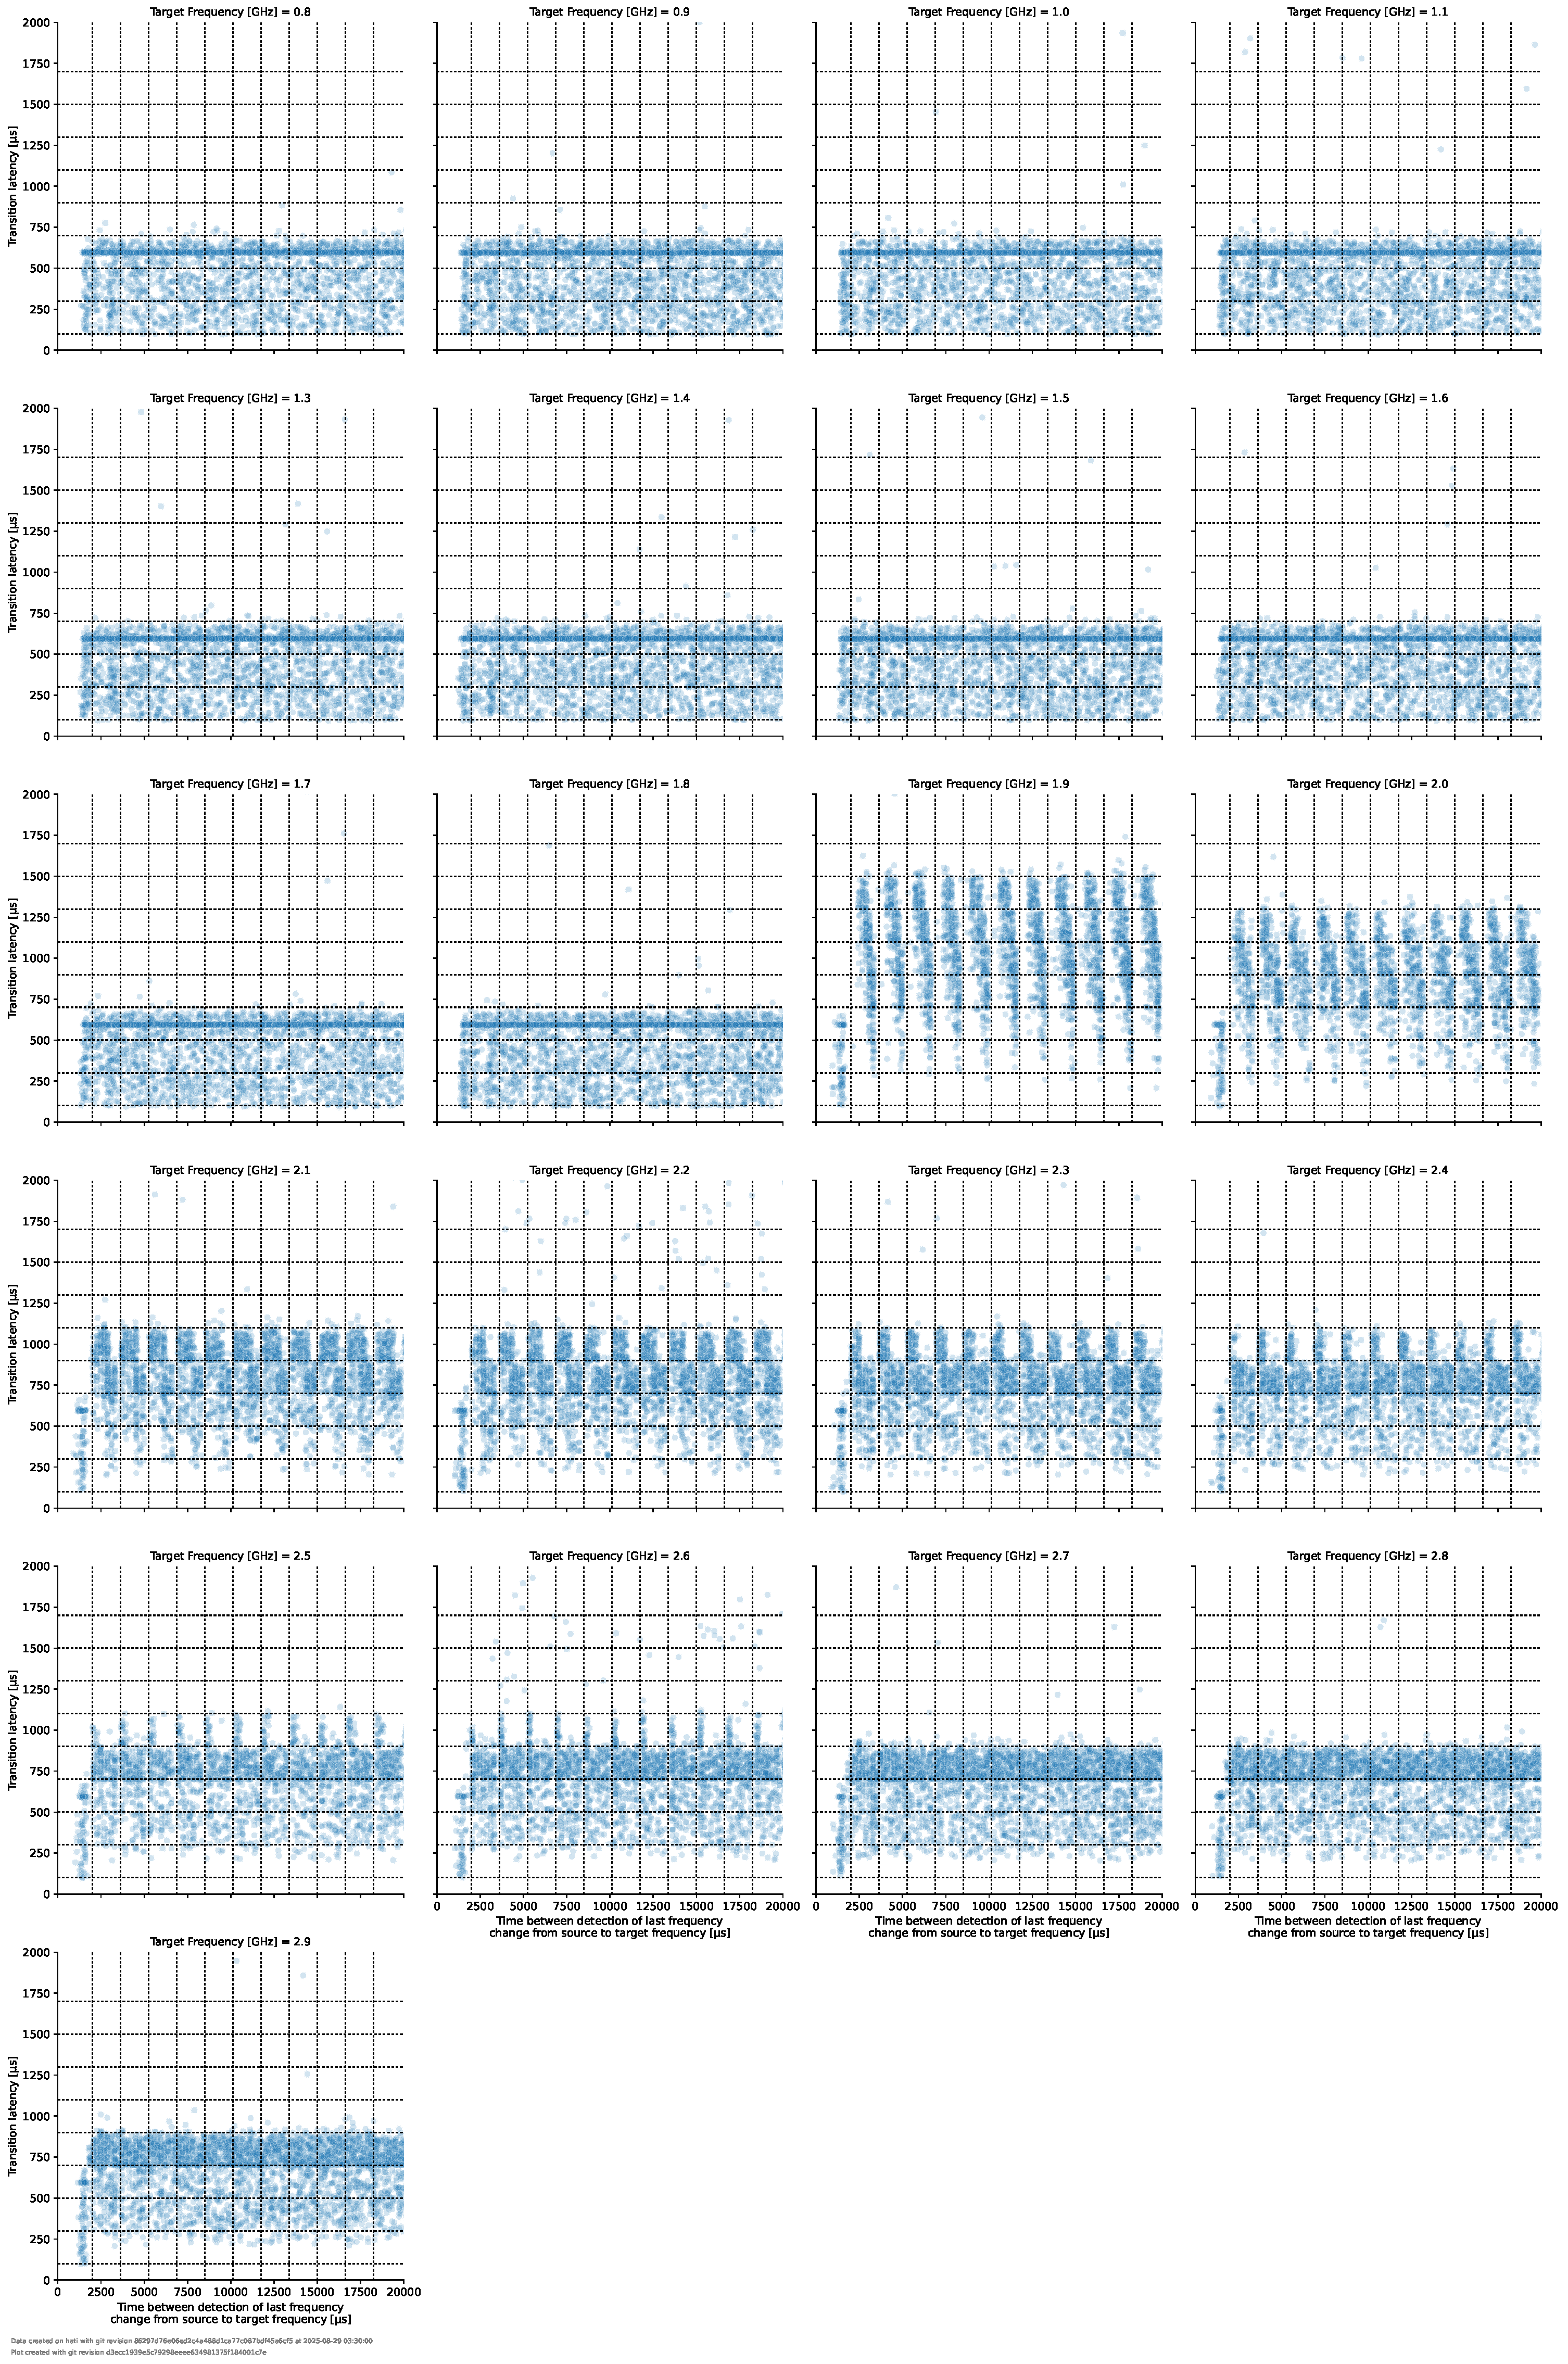
\includegraphics[width=\columnwidth]{fig/ftalat/ftalat_scatter_wait_transition_latency_hati_source_1.2.pdf}
    \caption{Dependance of the time between the detection events of transitions from \SI{1.2}{\GHz} to \SI{0.8}{}, \SI{0.9}{}, ..., \SI{2.9}{\GHz}. For better lines for bins of size \SI{1625}{\us} and \SI{200}{\us} have been included for the x and y-axis respectively.}
\end{figure}
\begin{figure}[]
    \centering
    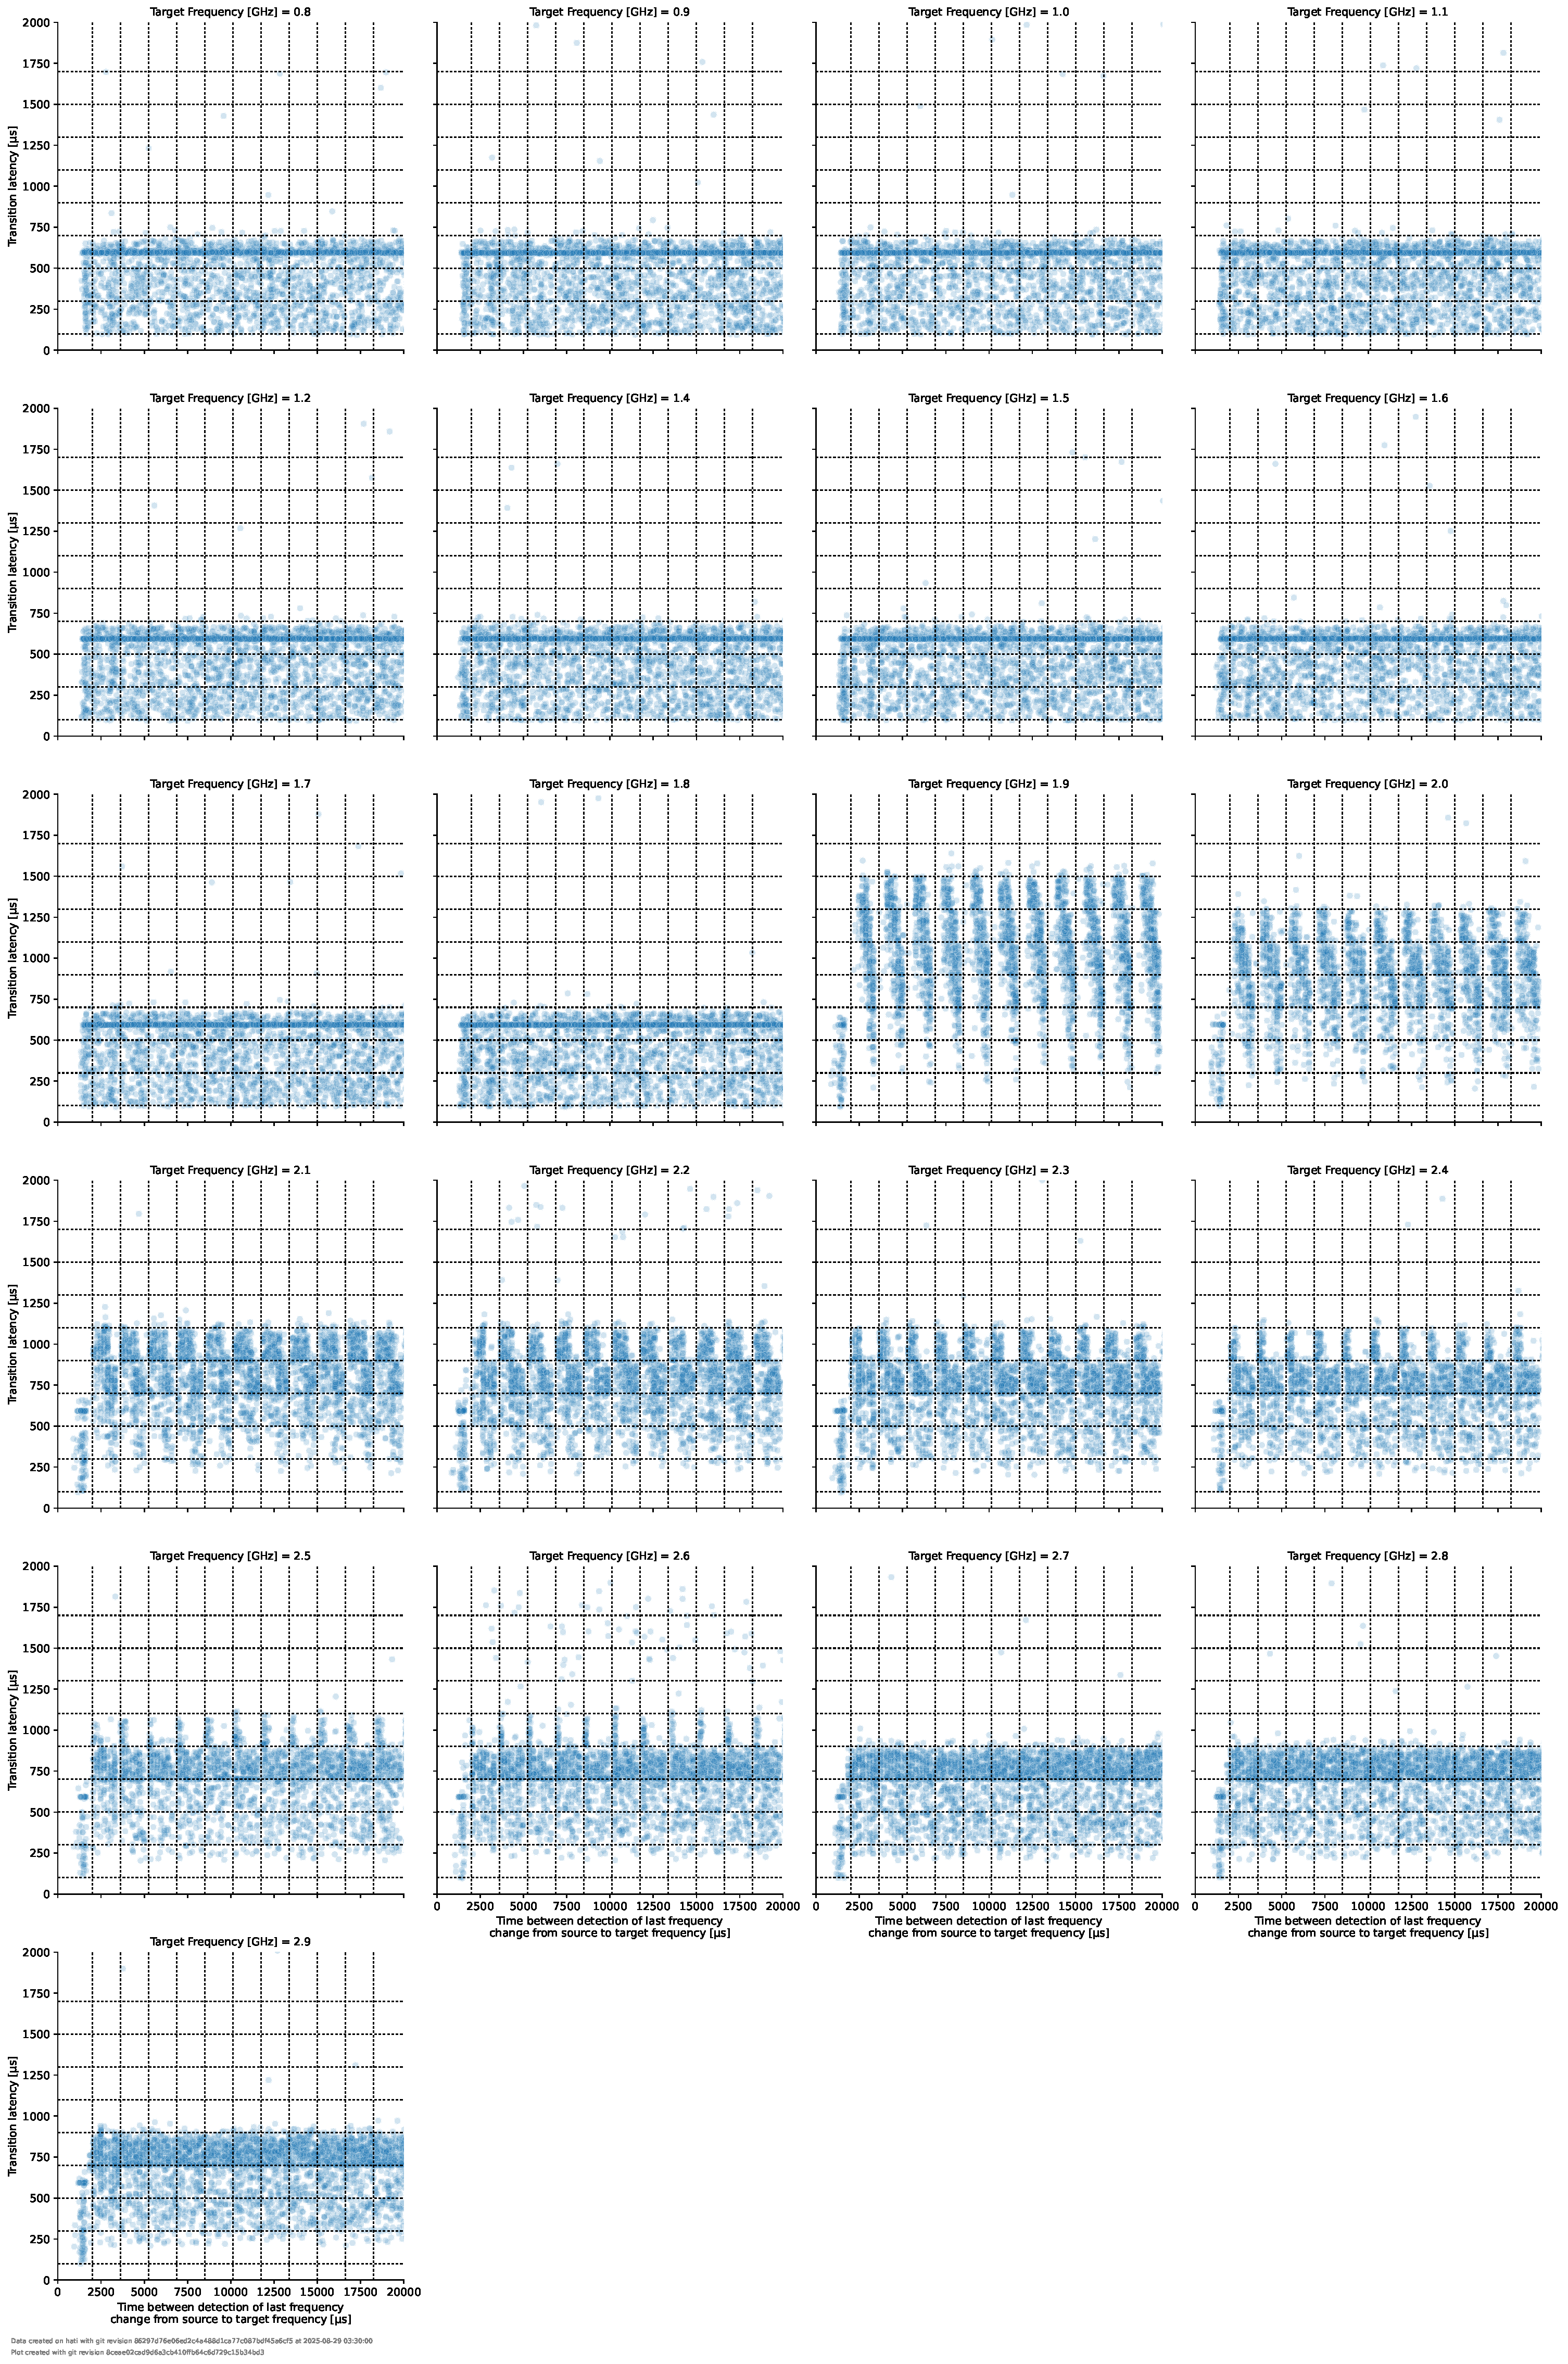
\includegraphics[width=\columnwidth]{fig/ftalat/ftalat_scatter_wait_transition_latency_hati_source_1.3.pdf}
    \caption{Dependance of the time between the detection events of transitions from \SI{1.3}{\GHz} to \SI{0.8}{}, \SI{0.9}{}, ..., \SI{2.9}{\GHz}. For better lines for bins of size \SI{1625}{\us} and \SI{200}{\us} have been included for the x and y-axis respectively.}
\end{figure}
\begin{figure}[]
    \centering
    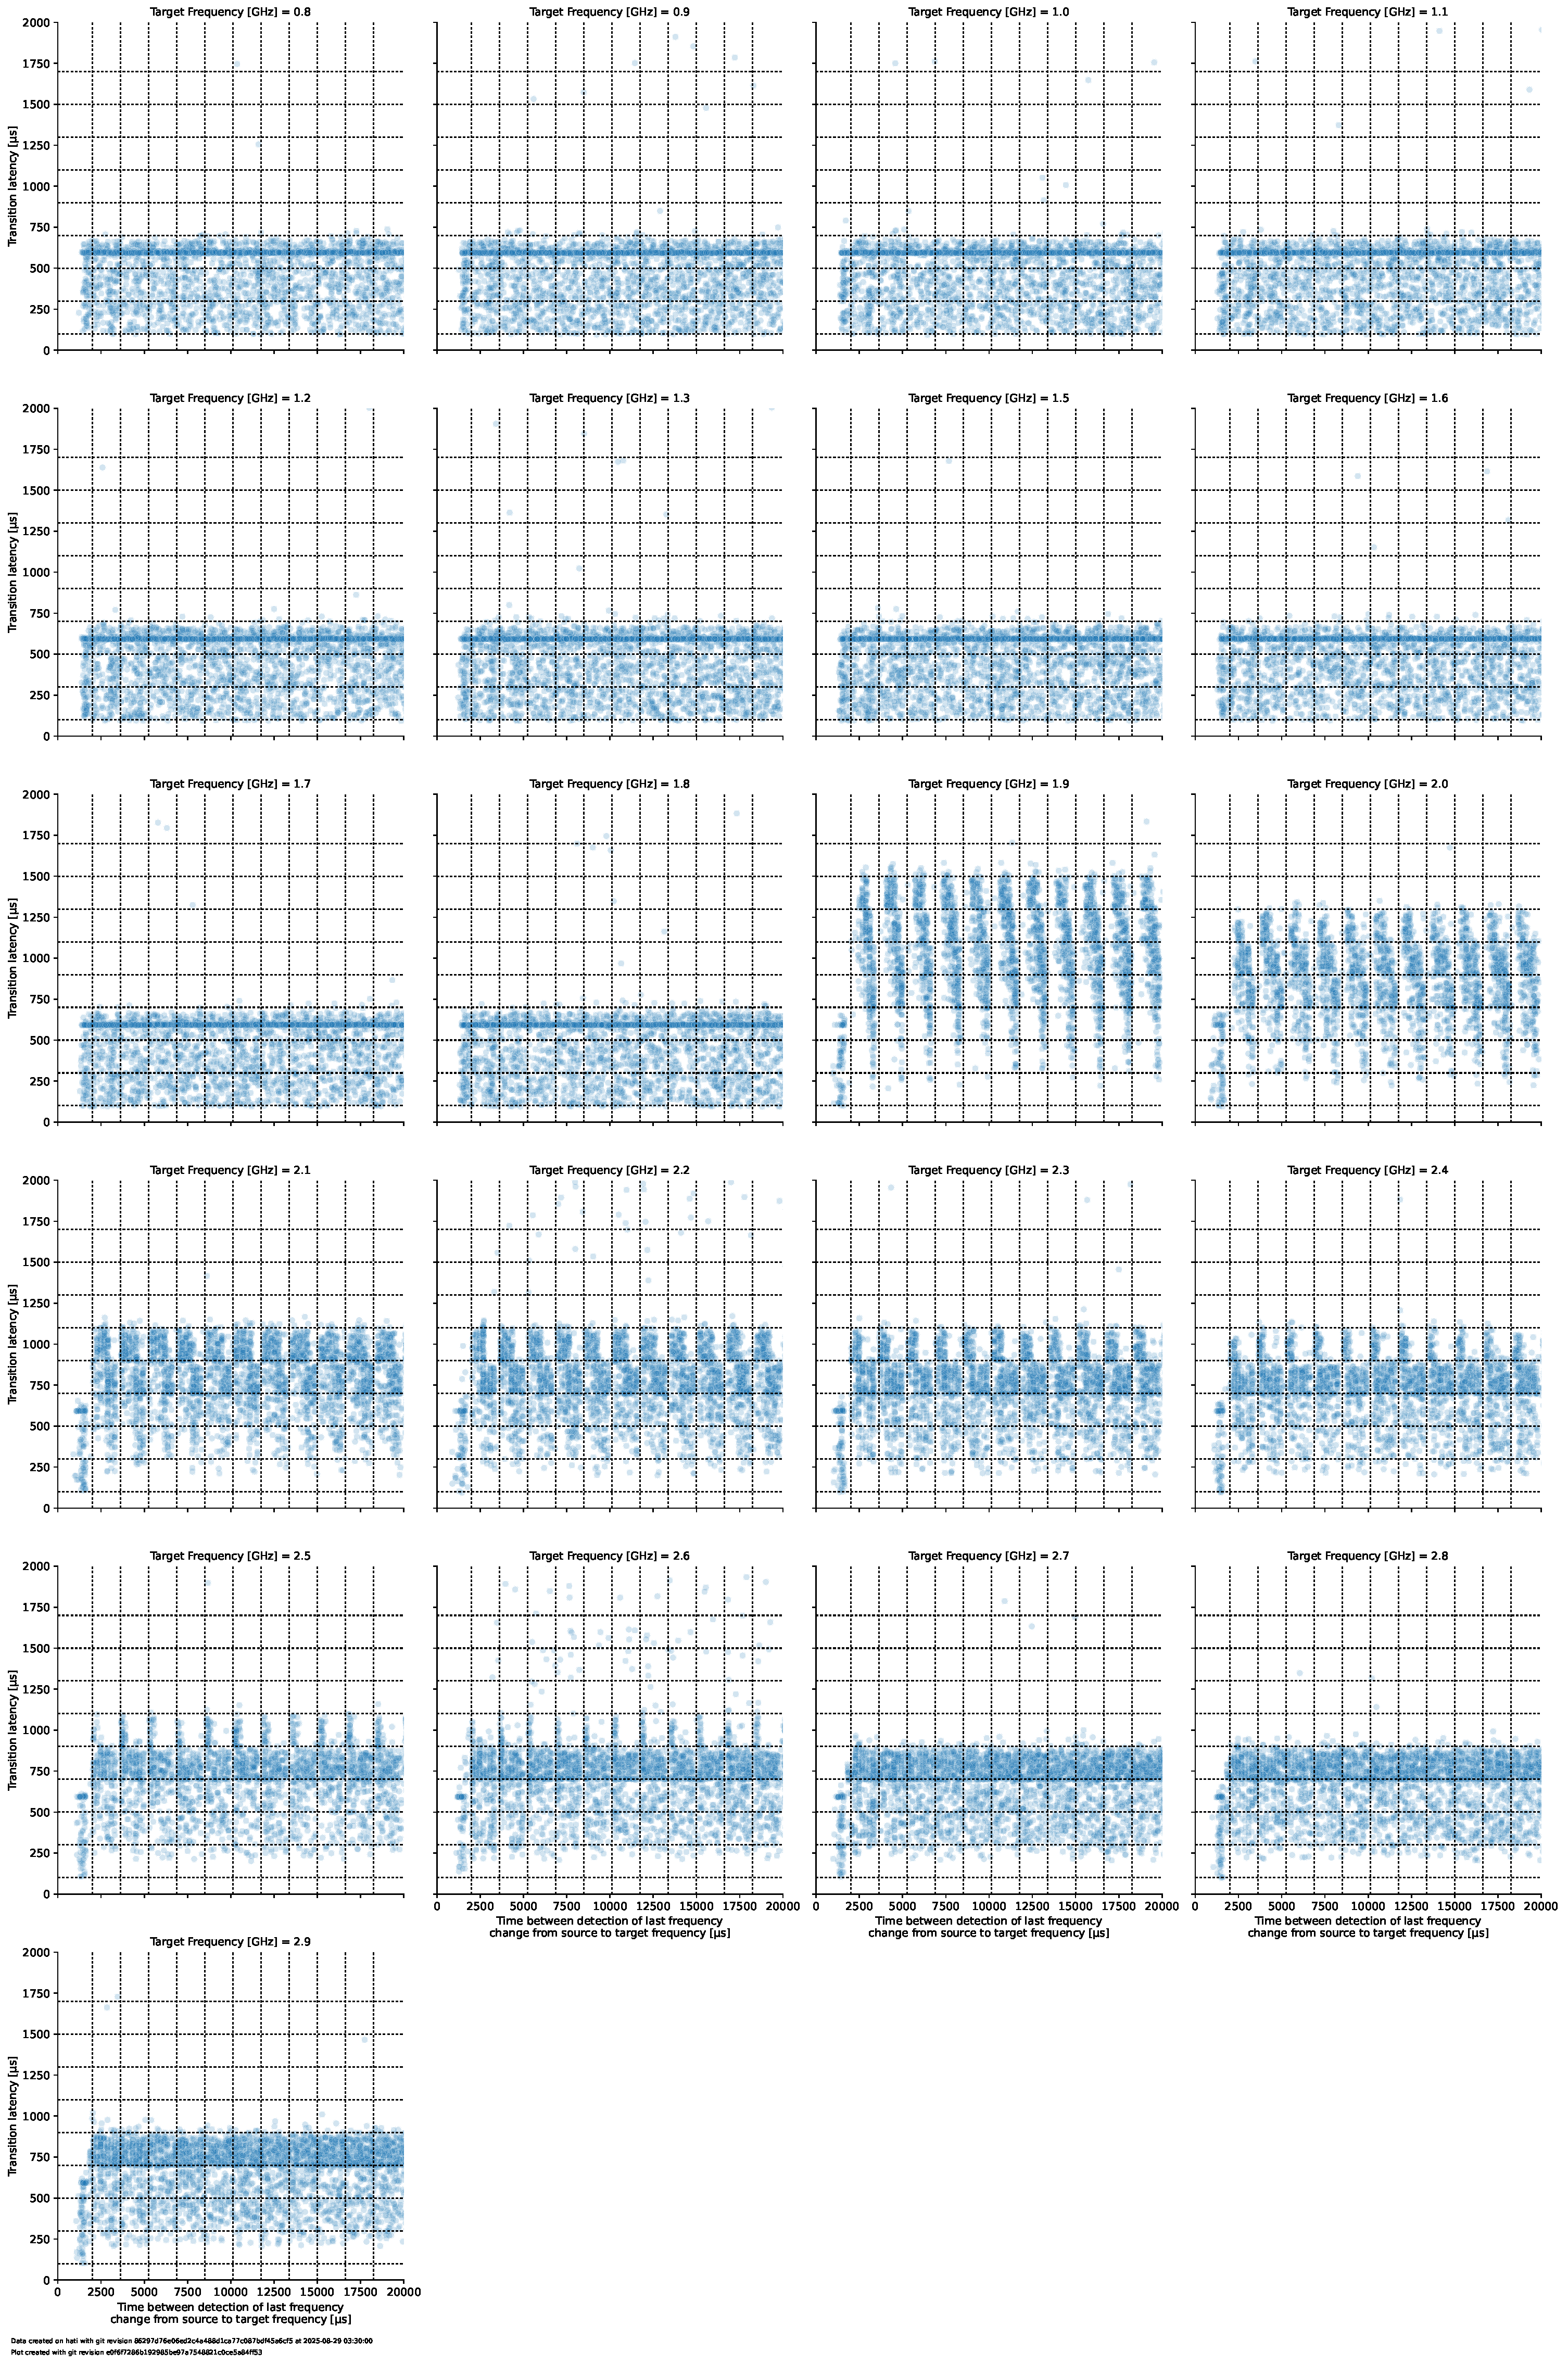
\includegraphics[width=\columnwidth]{fig/ftalat/ftalat_scatter_wait_transition_latency_hati_source_1.4.pdf}
    \caption{Dependance of the time between the detection events of transitions from \SI{1.4}{\GHz} to \SI{0.8}{}, \SI{0.9}{}, ..., \SI{2.9}{\GHz}. For better lines for bins of size \SI{1625}{\us} and \SI{200}{\us} have been included for the x and y-axis respectively.}
\end{figure}
\begin{figure}[]
    \centering
    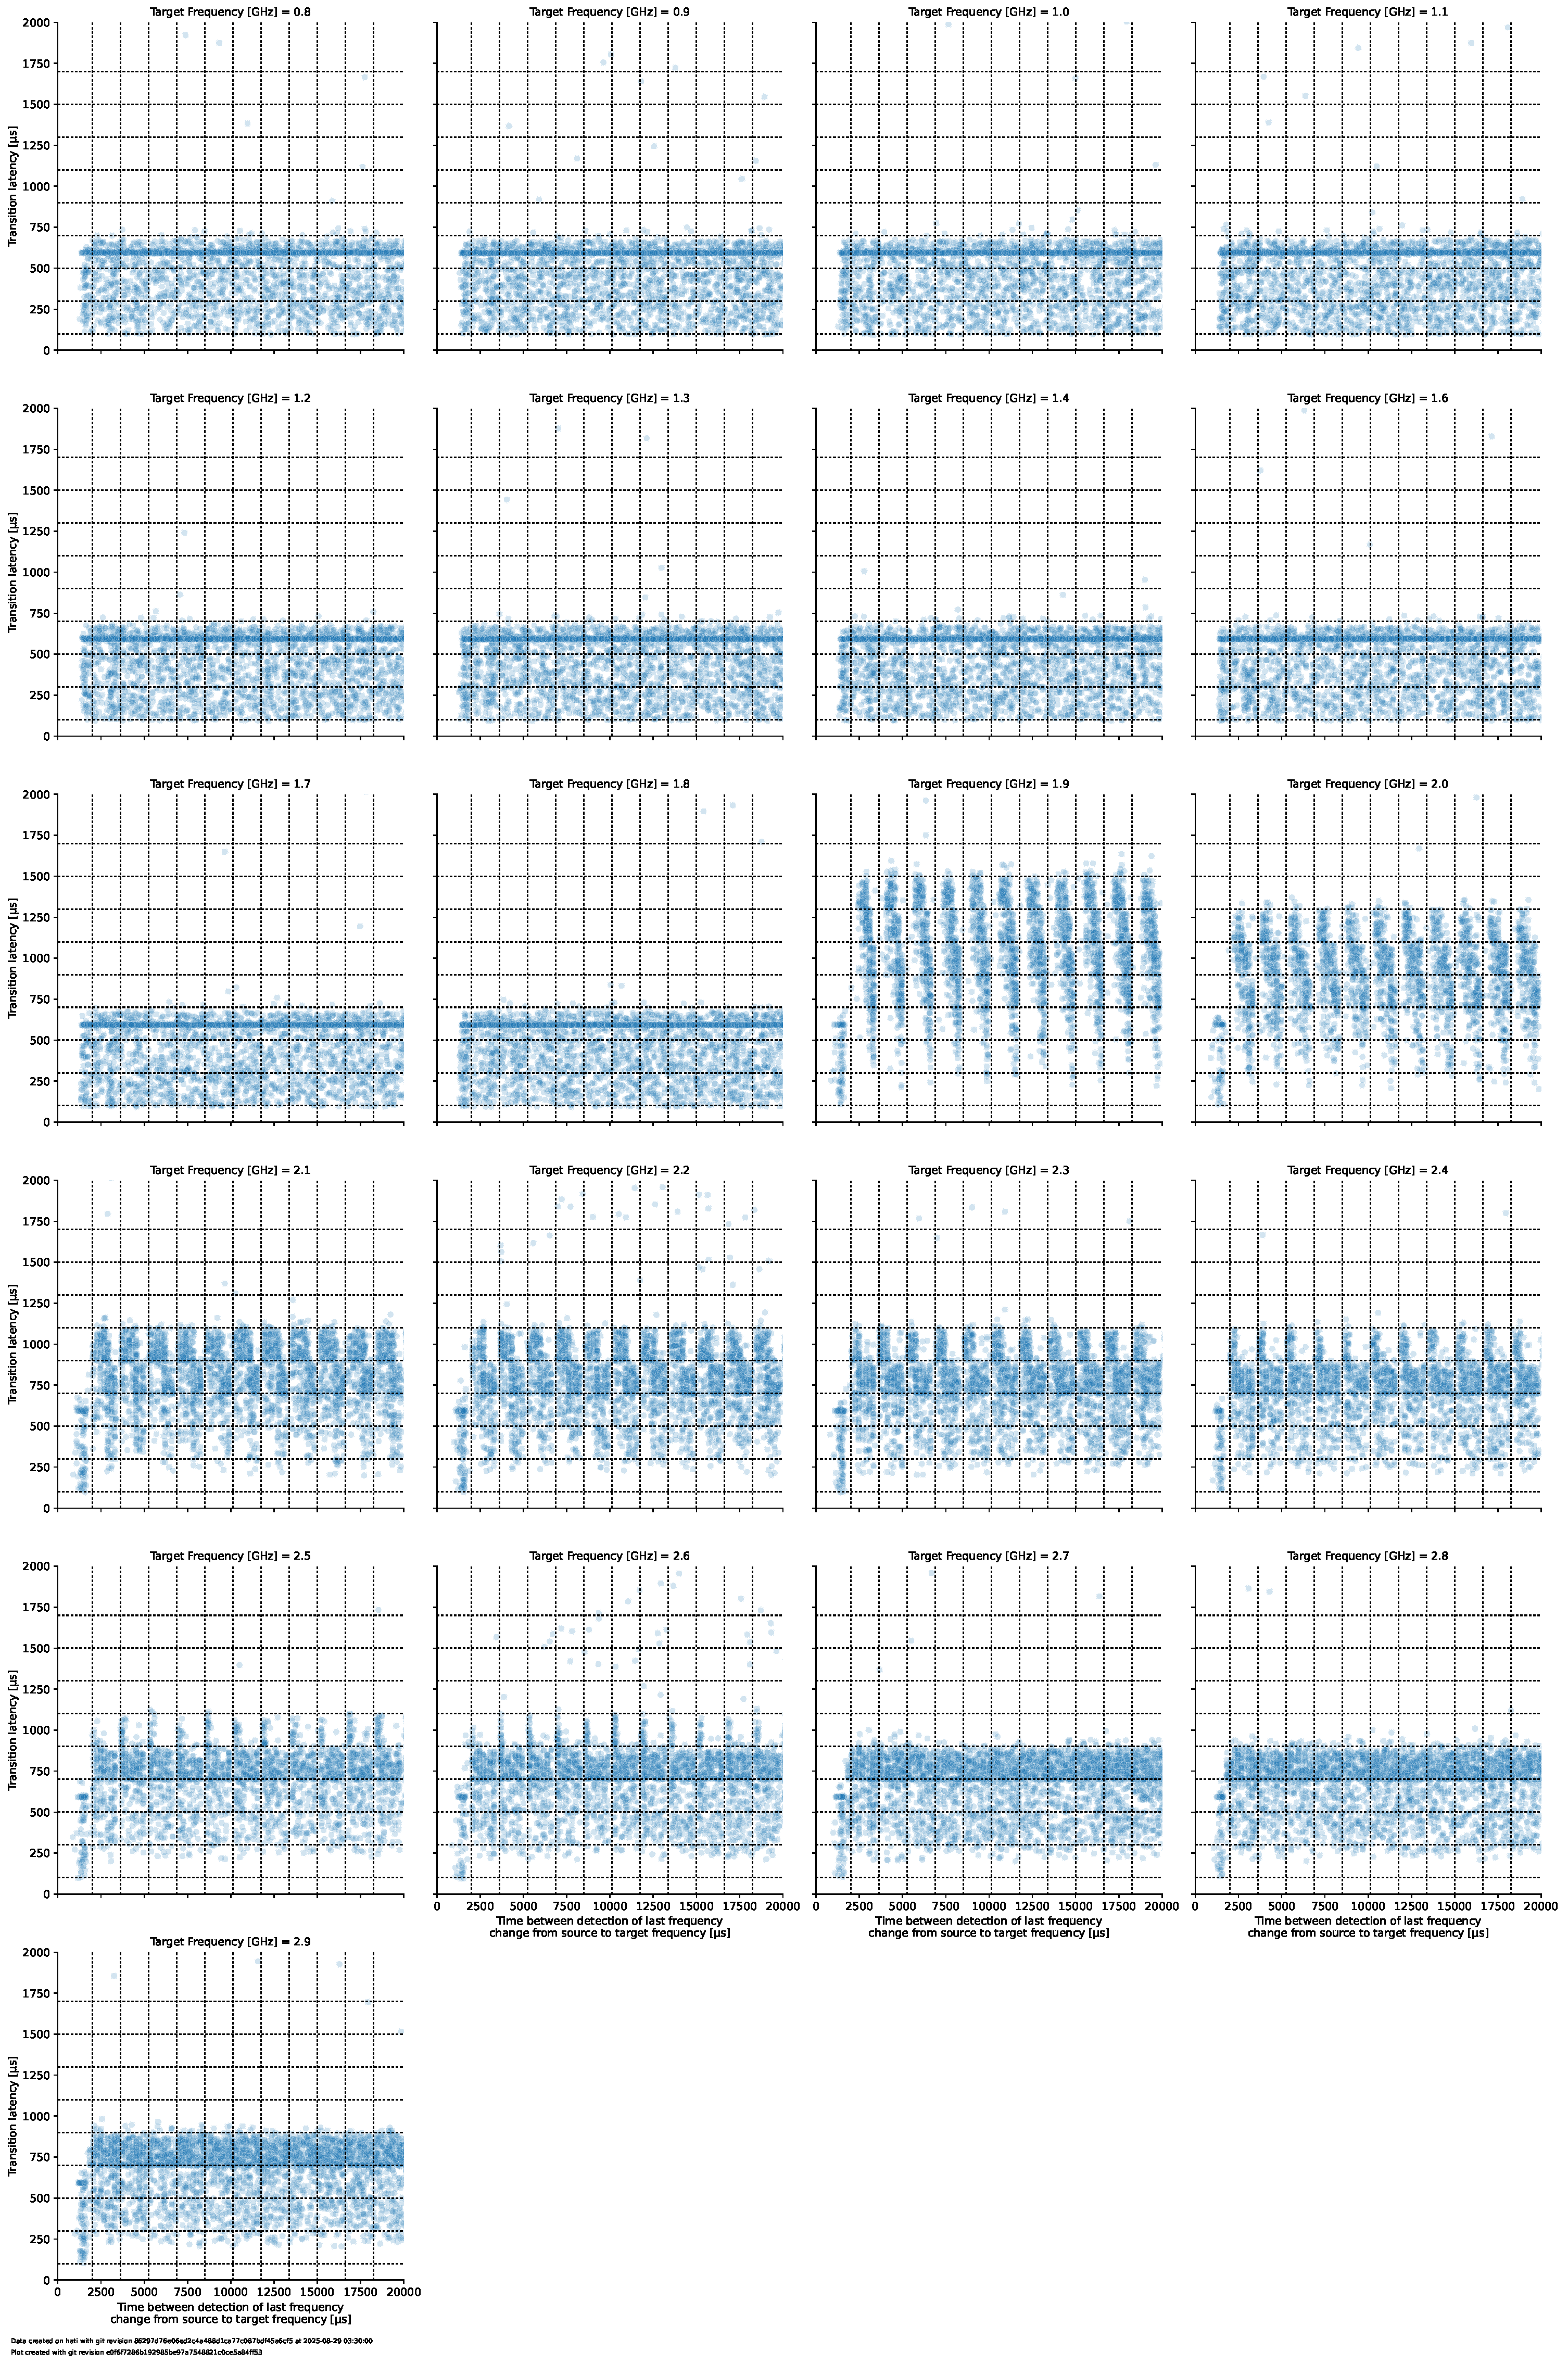
\includegraphics[width=\columnwidth]{fig/ftalat/ftalat_scatter_wait_transition_latency_hati_source_1.5.pdf}
    \caption{Dependance of the time between the detection events of transitions from \SI{1.5}{\GHz} to \SI{0.8}{}, \SI{0.9}{}, ..., \SI{2.9}{\GHz}. For better lines for bins of size \SI{1625}{\us} and \SI{200}{\us} have been included for the x and y-axis respectively.}
\end{figure}
\begin{figure}[]
    \centering
    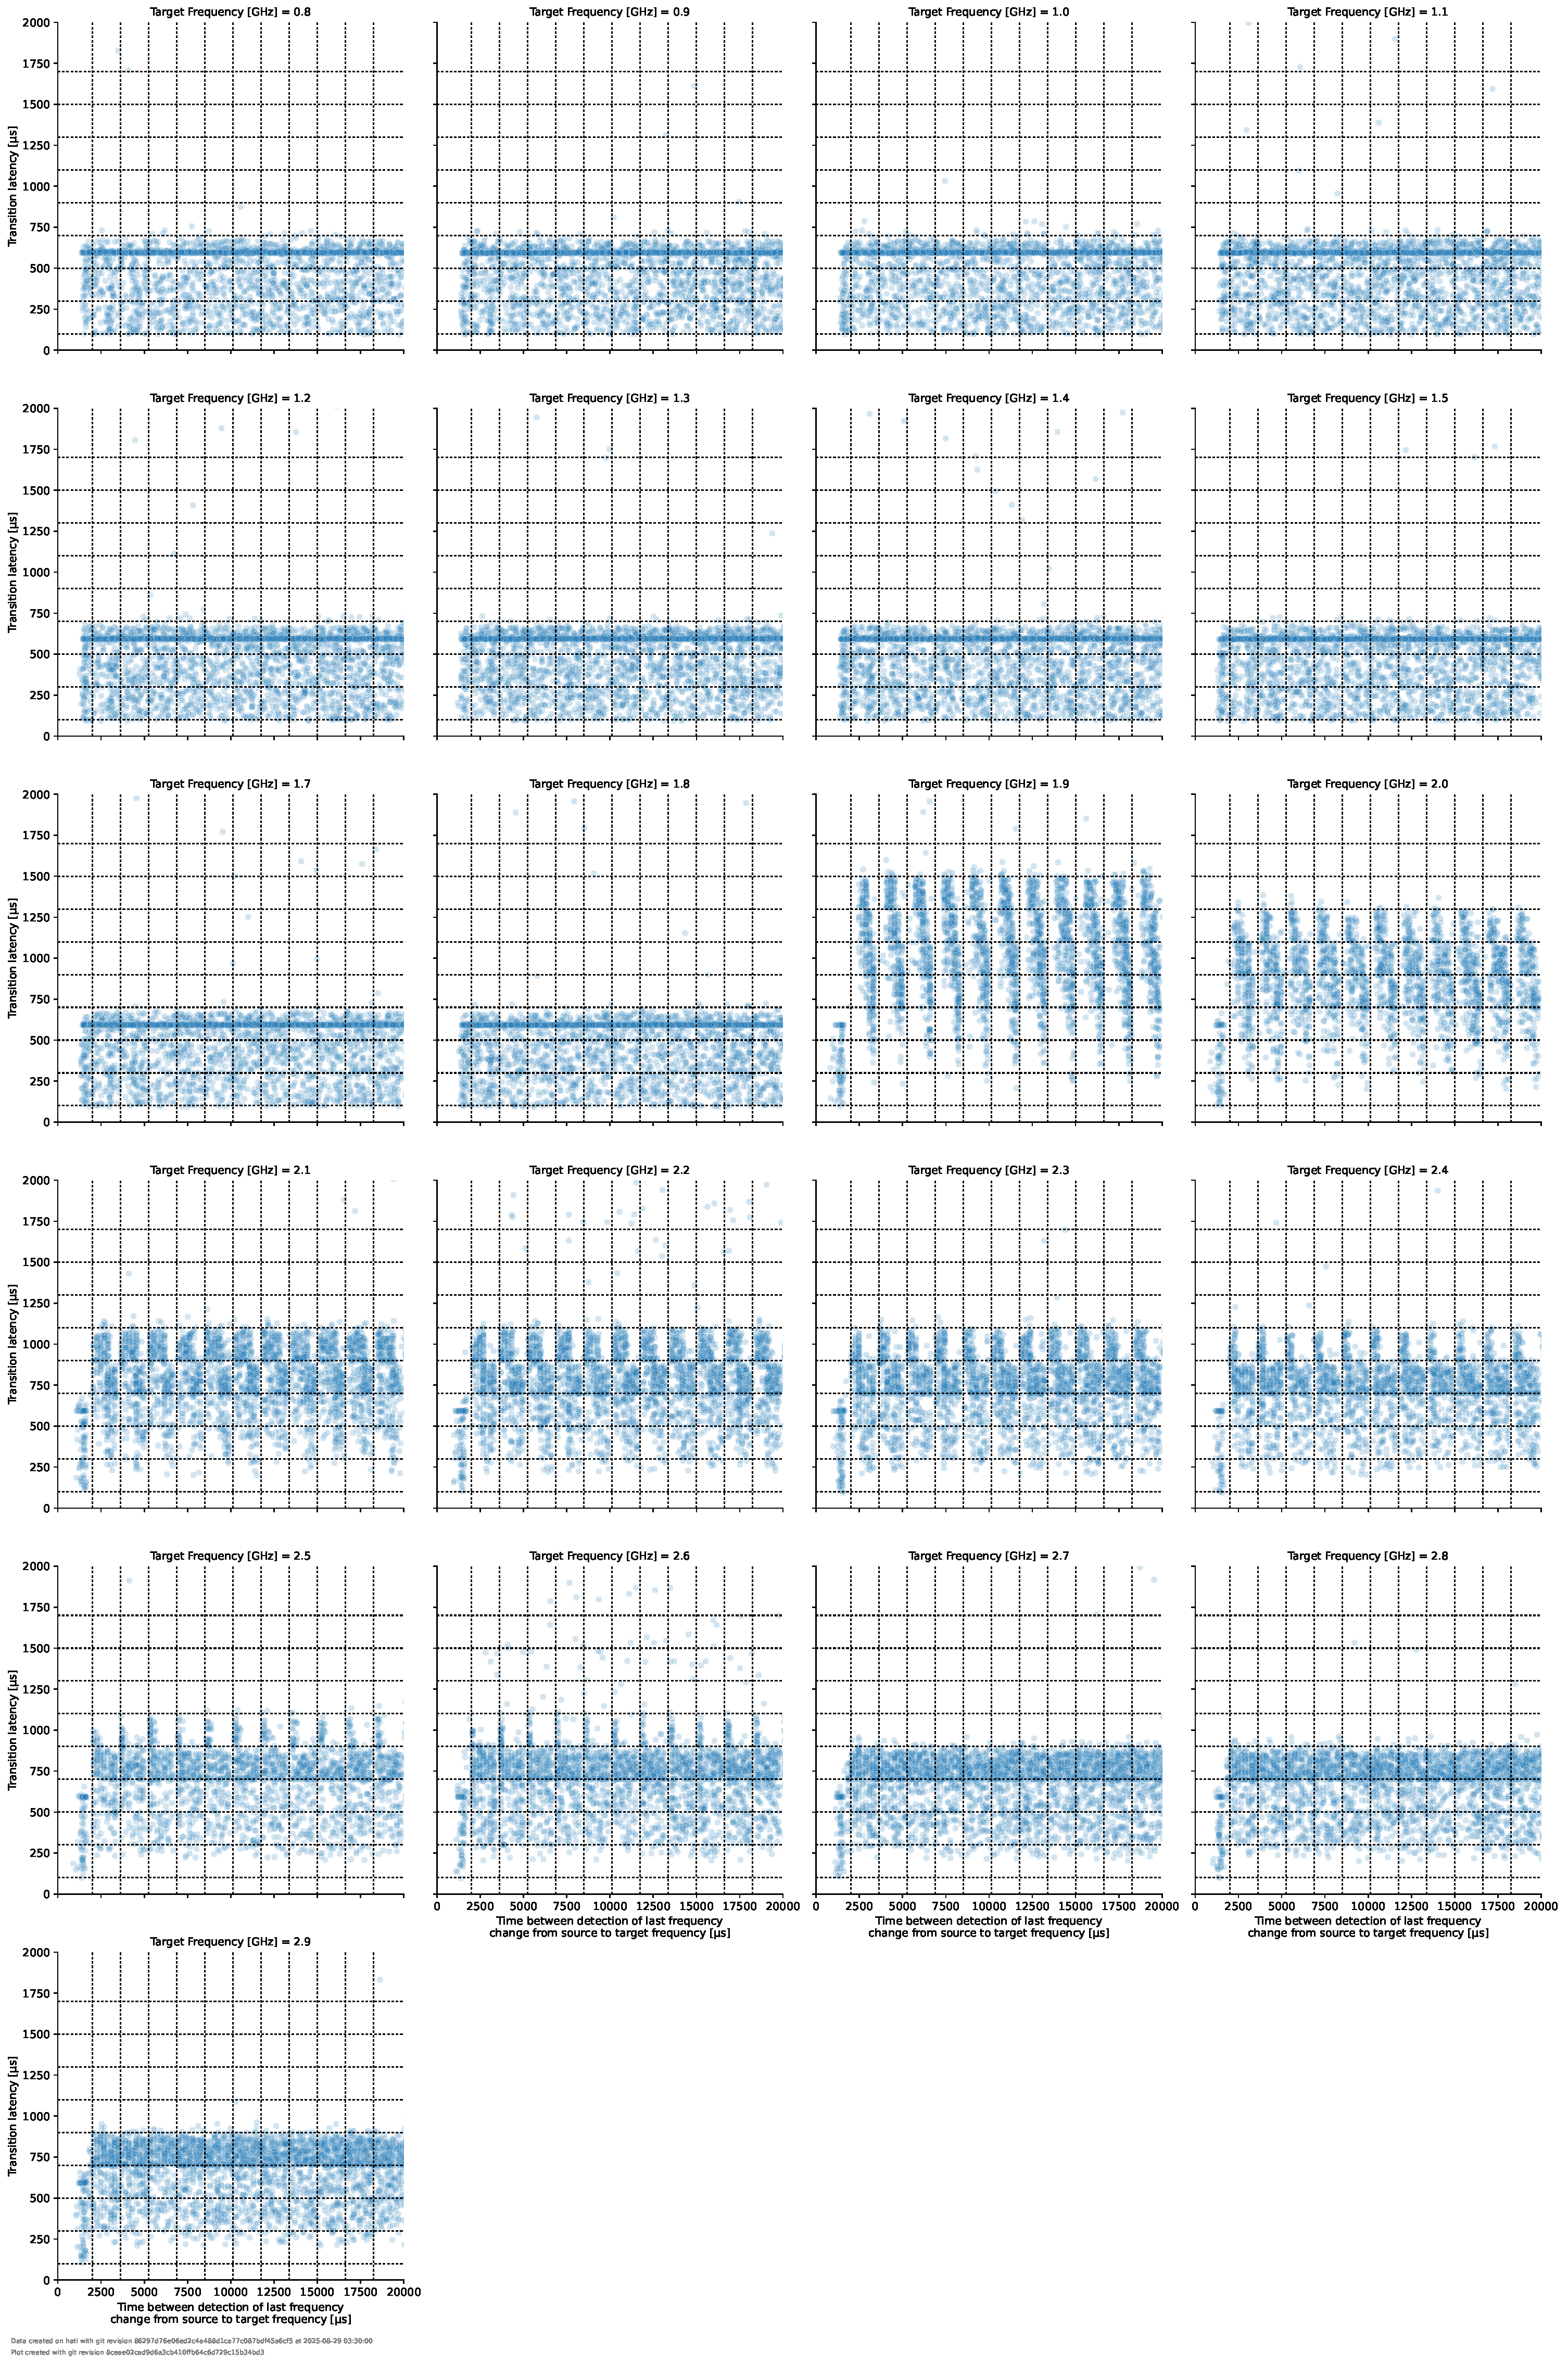
\includegraphics[width=\columnwidth]{fig/ftalat/ftalat_scatter_wait_transition_latency_hati_source_1.6.pdf}
    \caption{Dependance of the time between the detection events of transitions from \SI{1.6}{\GHz} to \SI{0.8}{}, \SI{0.9}{}, ..., \SI{2.9}{\GHz}. For better lines for bins of size \SI{1625}{\us} and \SI{200}{\us} have been included for the x and y-axis respectively.}
\end{figure}
\begin{figure}[]
    \centering
    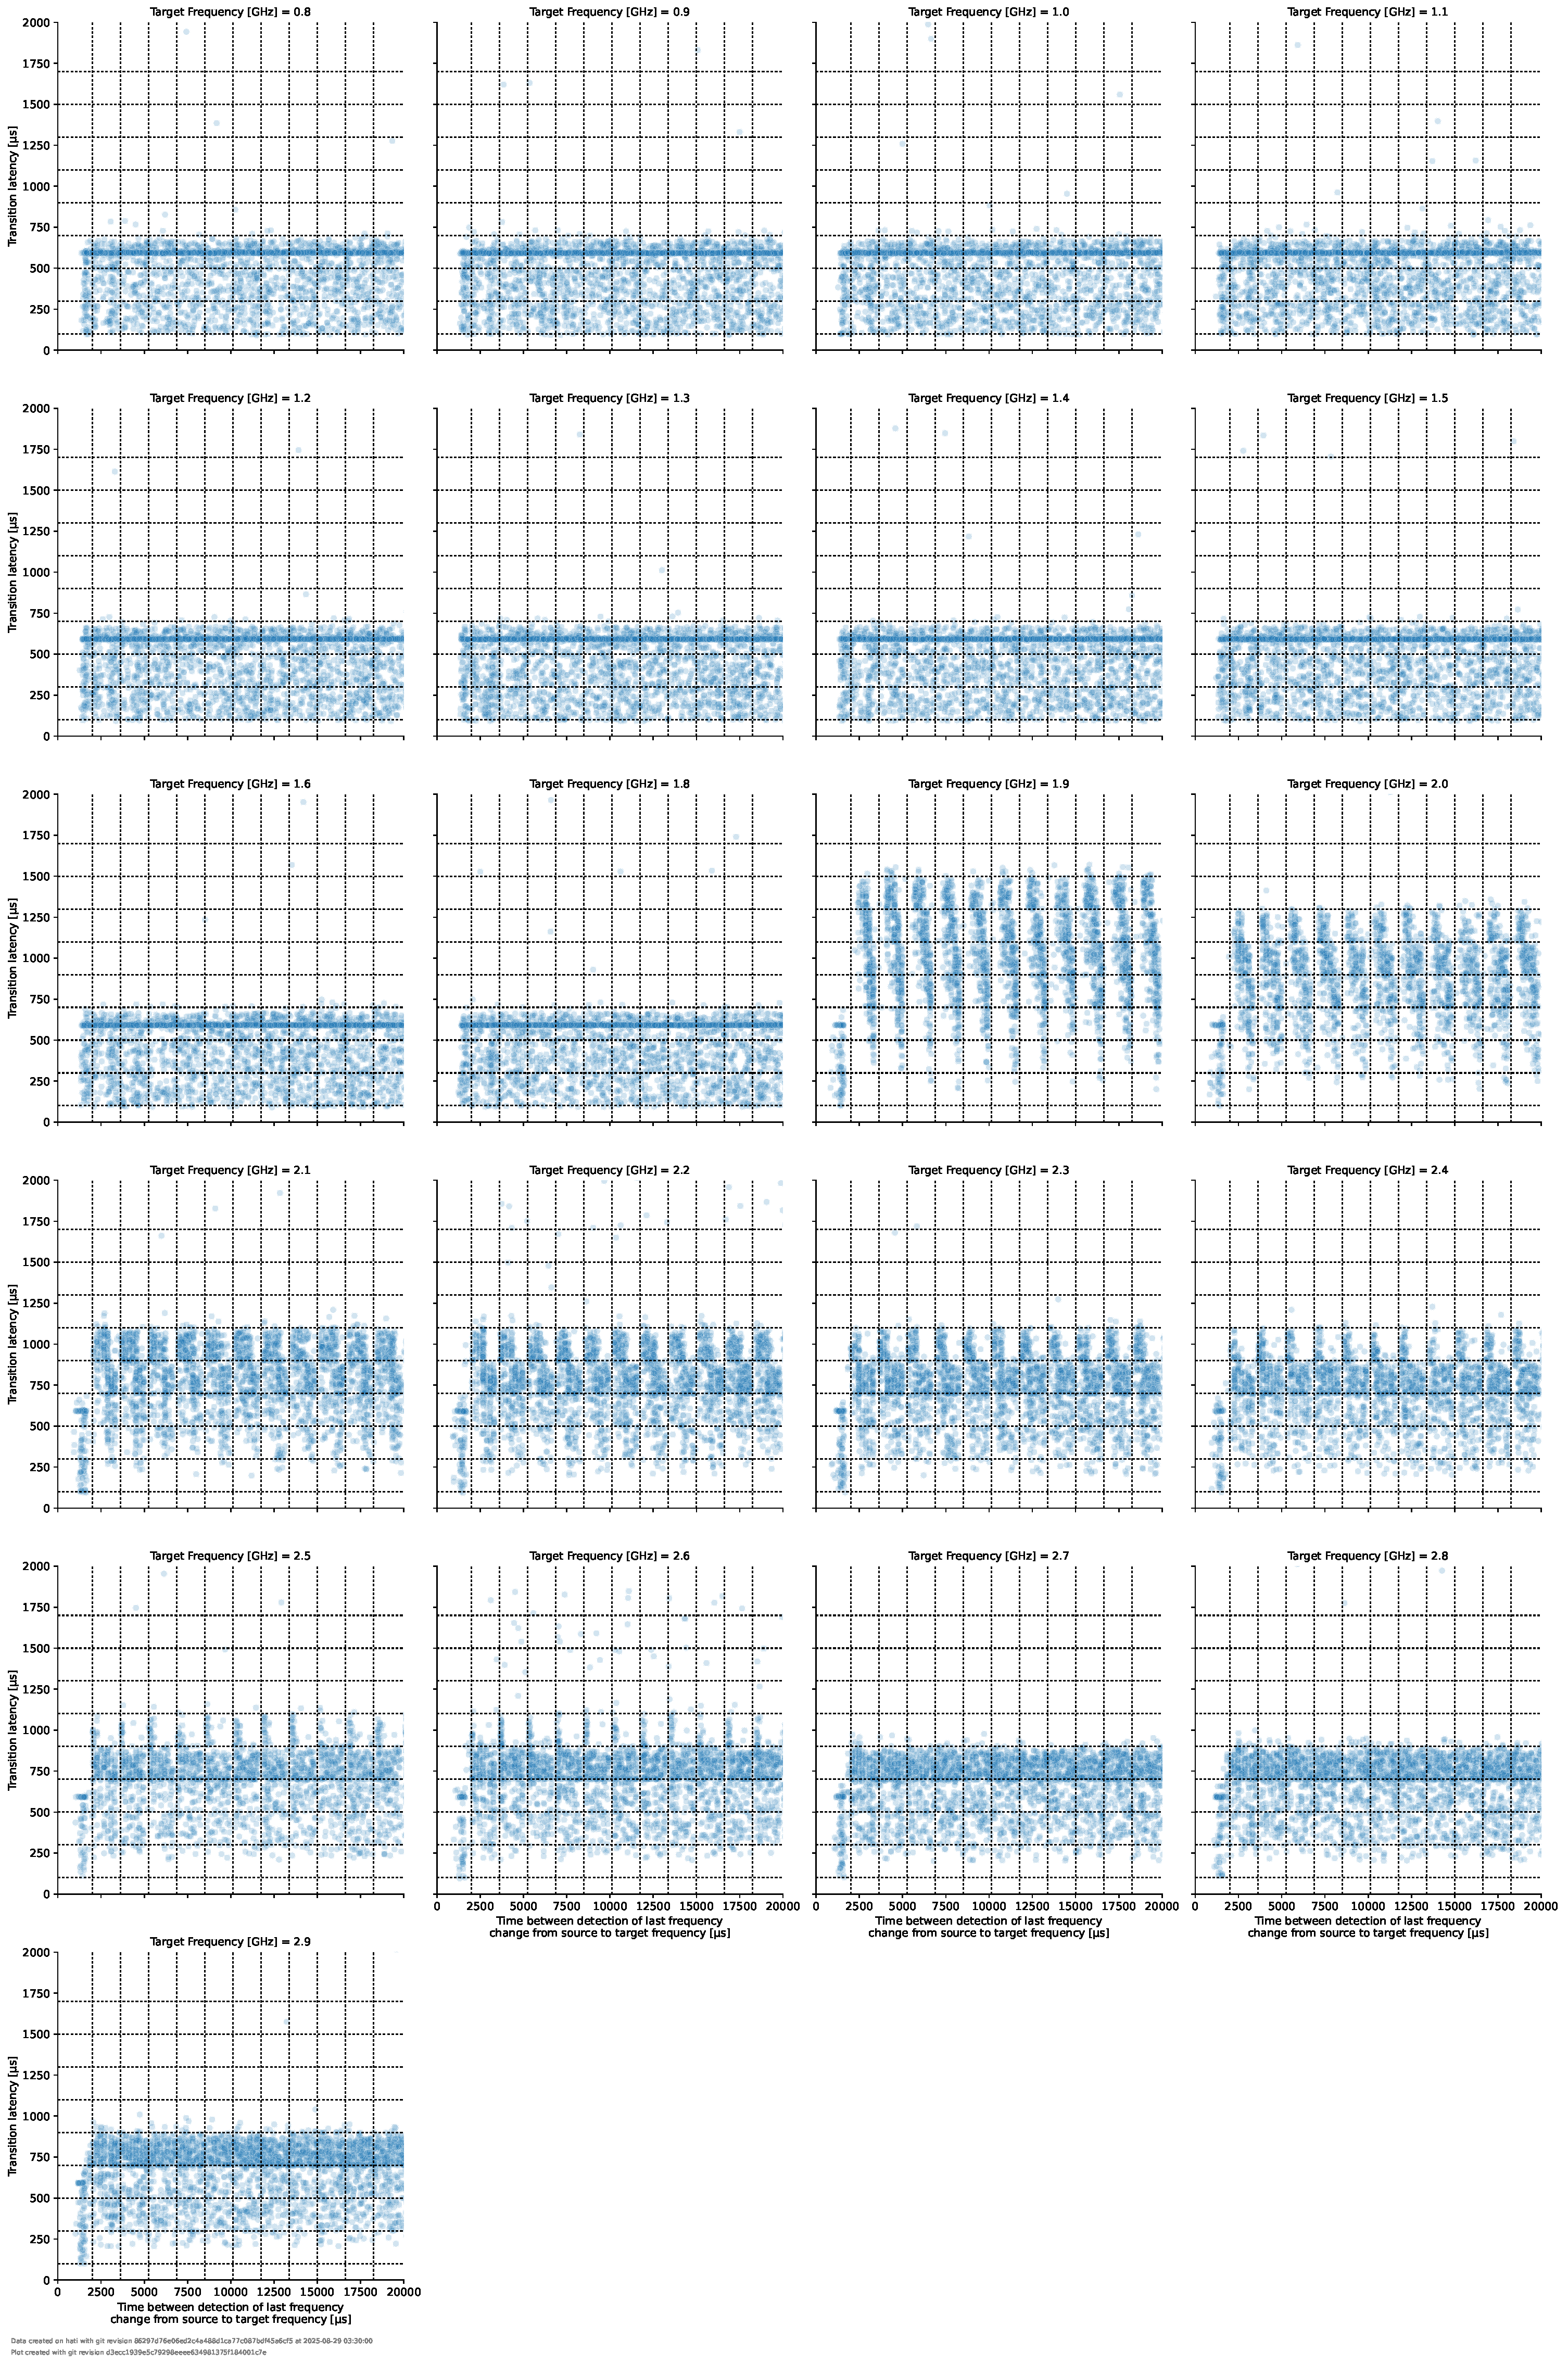
\includegraphics[width=\columnwidth]{fig/ftalat/ftalat_scatter_wait_transition_latency_hati_source_1.7.pdf}
    \caption{Dependance of the time between the detection events of transitions from \SI{1.7}{\GHz} to \SI{0.8}{}, \SI{0.9}{}, ..., \SI{2.9}{\GHz}. For better lines for bins of size \SI{1625}{\us} and \SI{200}{\us} have been included for the x and y-axis respectively.}
\end{figure}
\begin{figure}[]
    \centering
    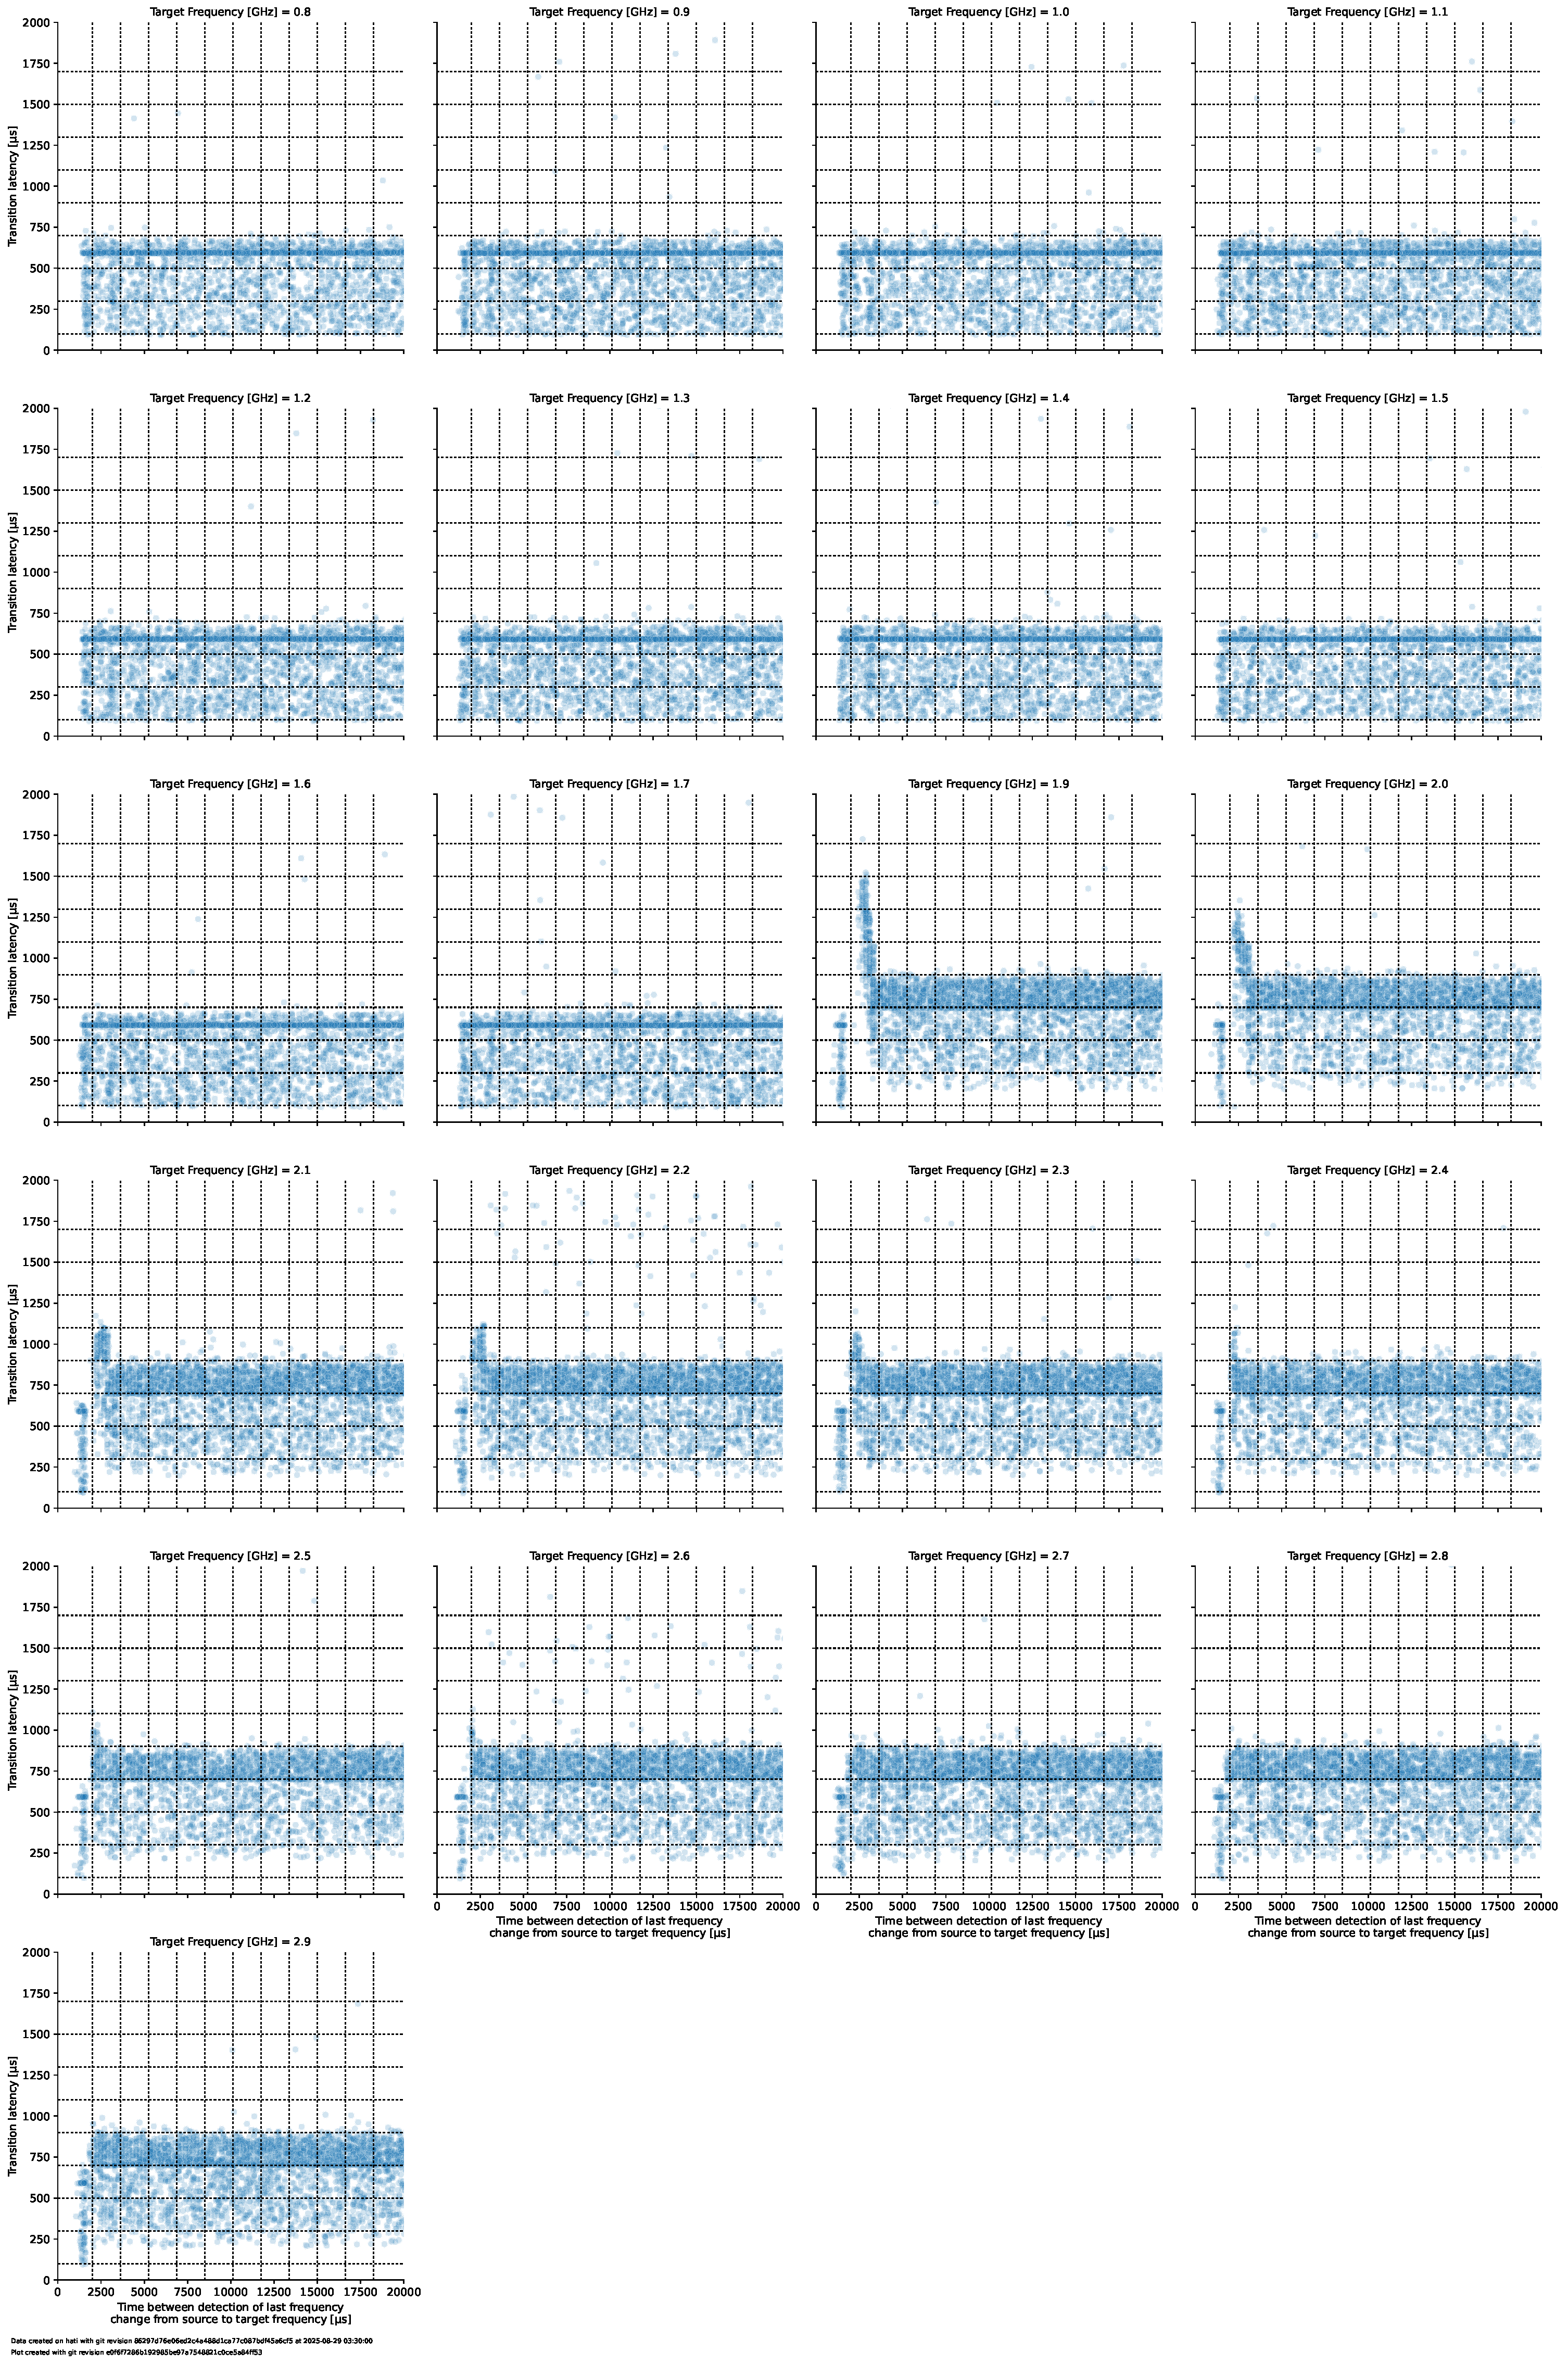
\includegraphics[width=\columnwidth]{fig/ftalat/ftalat_scatter_wait_transition_latency_hati_source_1.8.pdf}
    \caption{Dependance of the time between the detection events of transitions from \SI{1.8}{\GHz} to \SI{0.8}{}, \SI{0.9}{}, ..., \SI{2.9}{\GHz}. For better lines for bins of size \SI{1625}{\us} and \SI{200}{\us} have been included for the x and y-axis respectively.}
\end{figure}
\begin{figure}[]
    \centering
    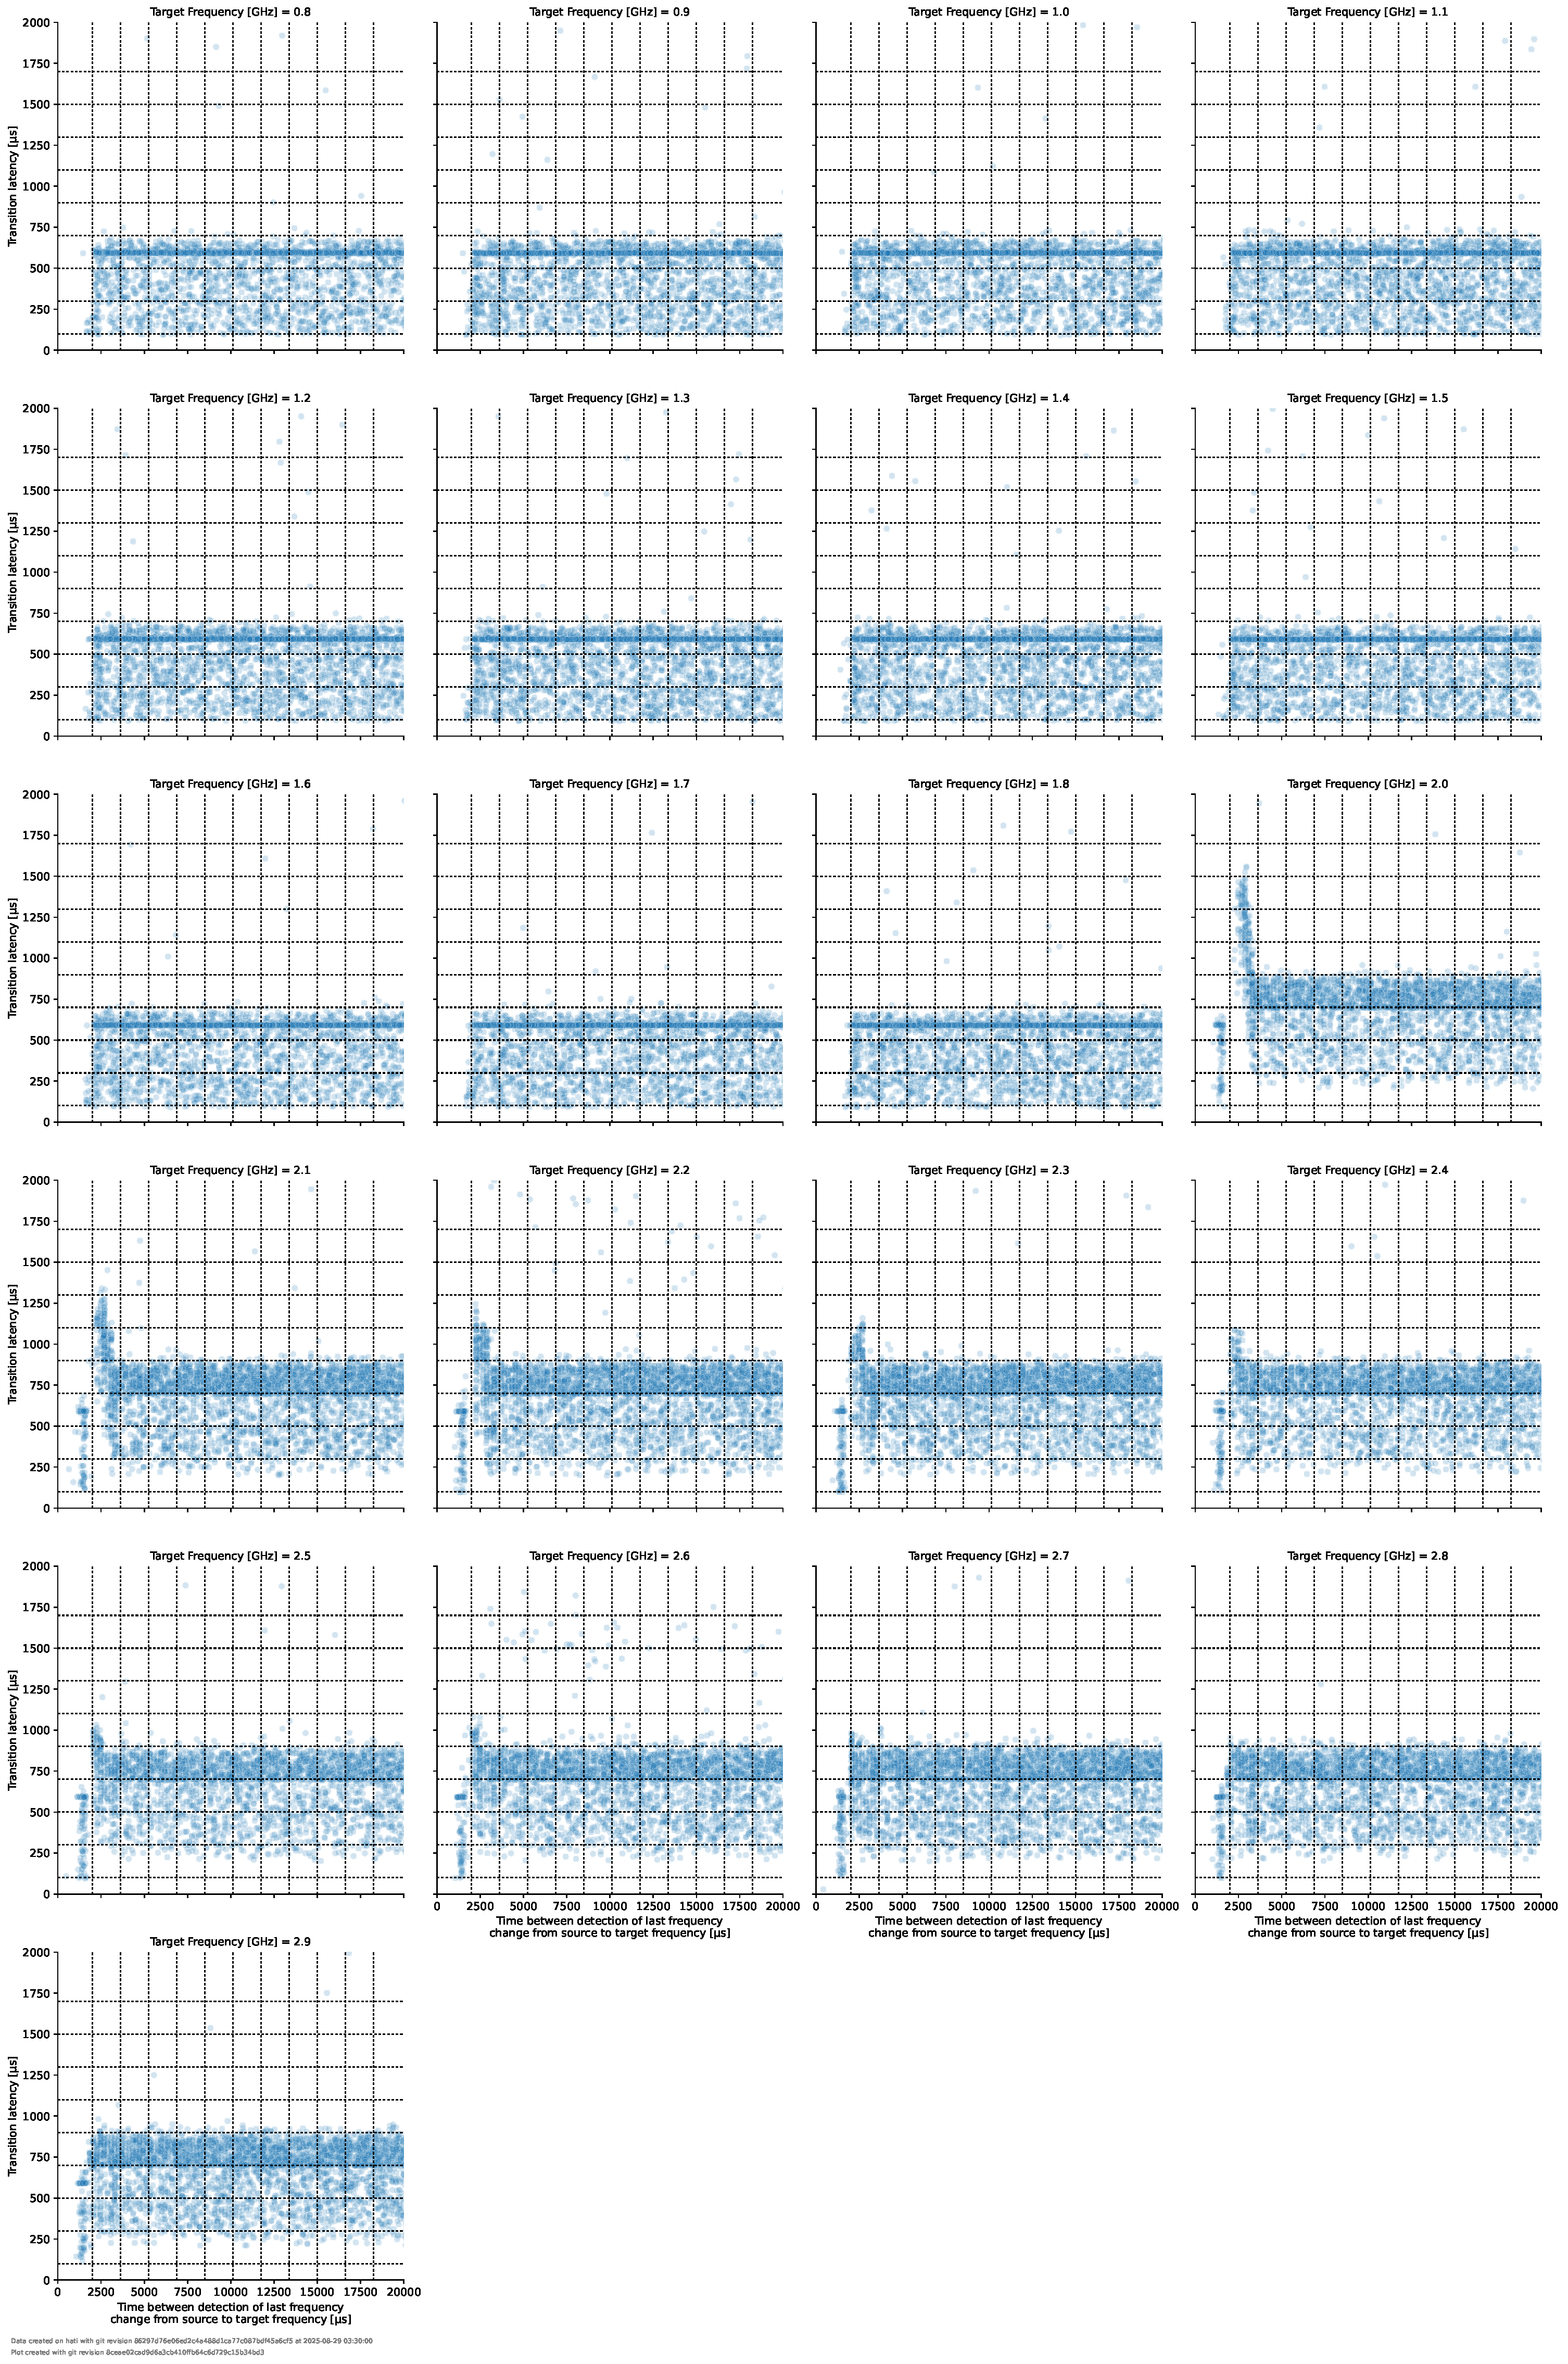
\includegraphics[width=\columnwidth]{fig/ftalat/ftalat_scatter_wait_transition_latency_hati_source_1.9.pdf}
    \caption{Dependance of the time between the detection events of transitions from \SI{1.9}{\GHz} to \SI{0.8}{}, \SI{0.9}{}, ..., \SI{2.9}{\GHz}. For better lines for bins of size \SI{1625}{\us} and \SI{200}{\us} have been included for the x and y-axis respectively.}
\end{figure}
\begin{figure}[]
    \centering
    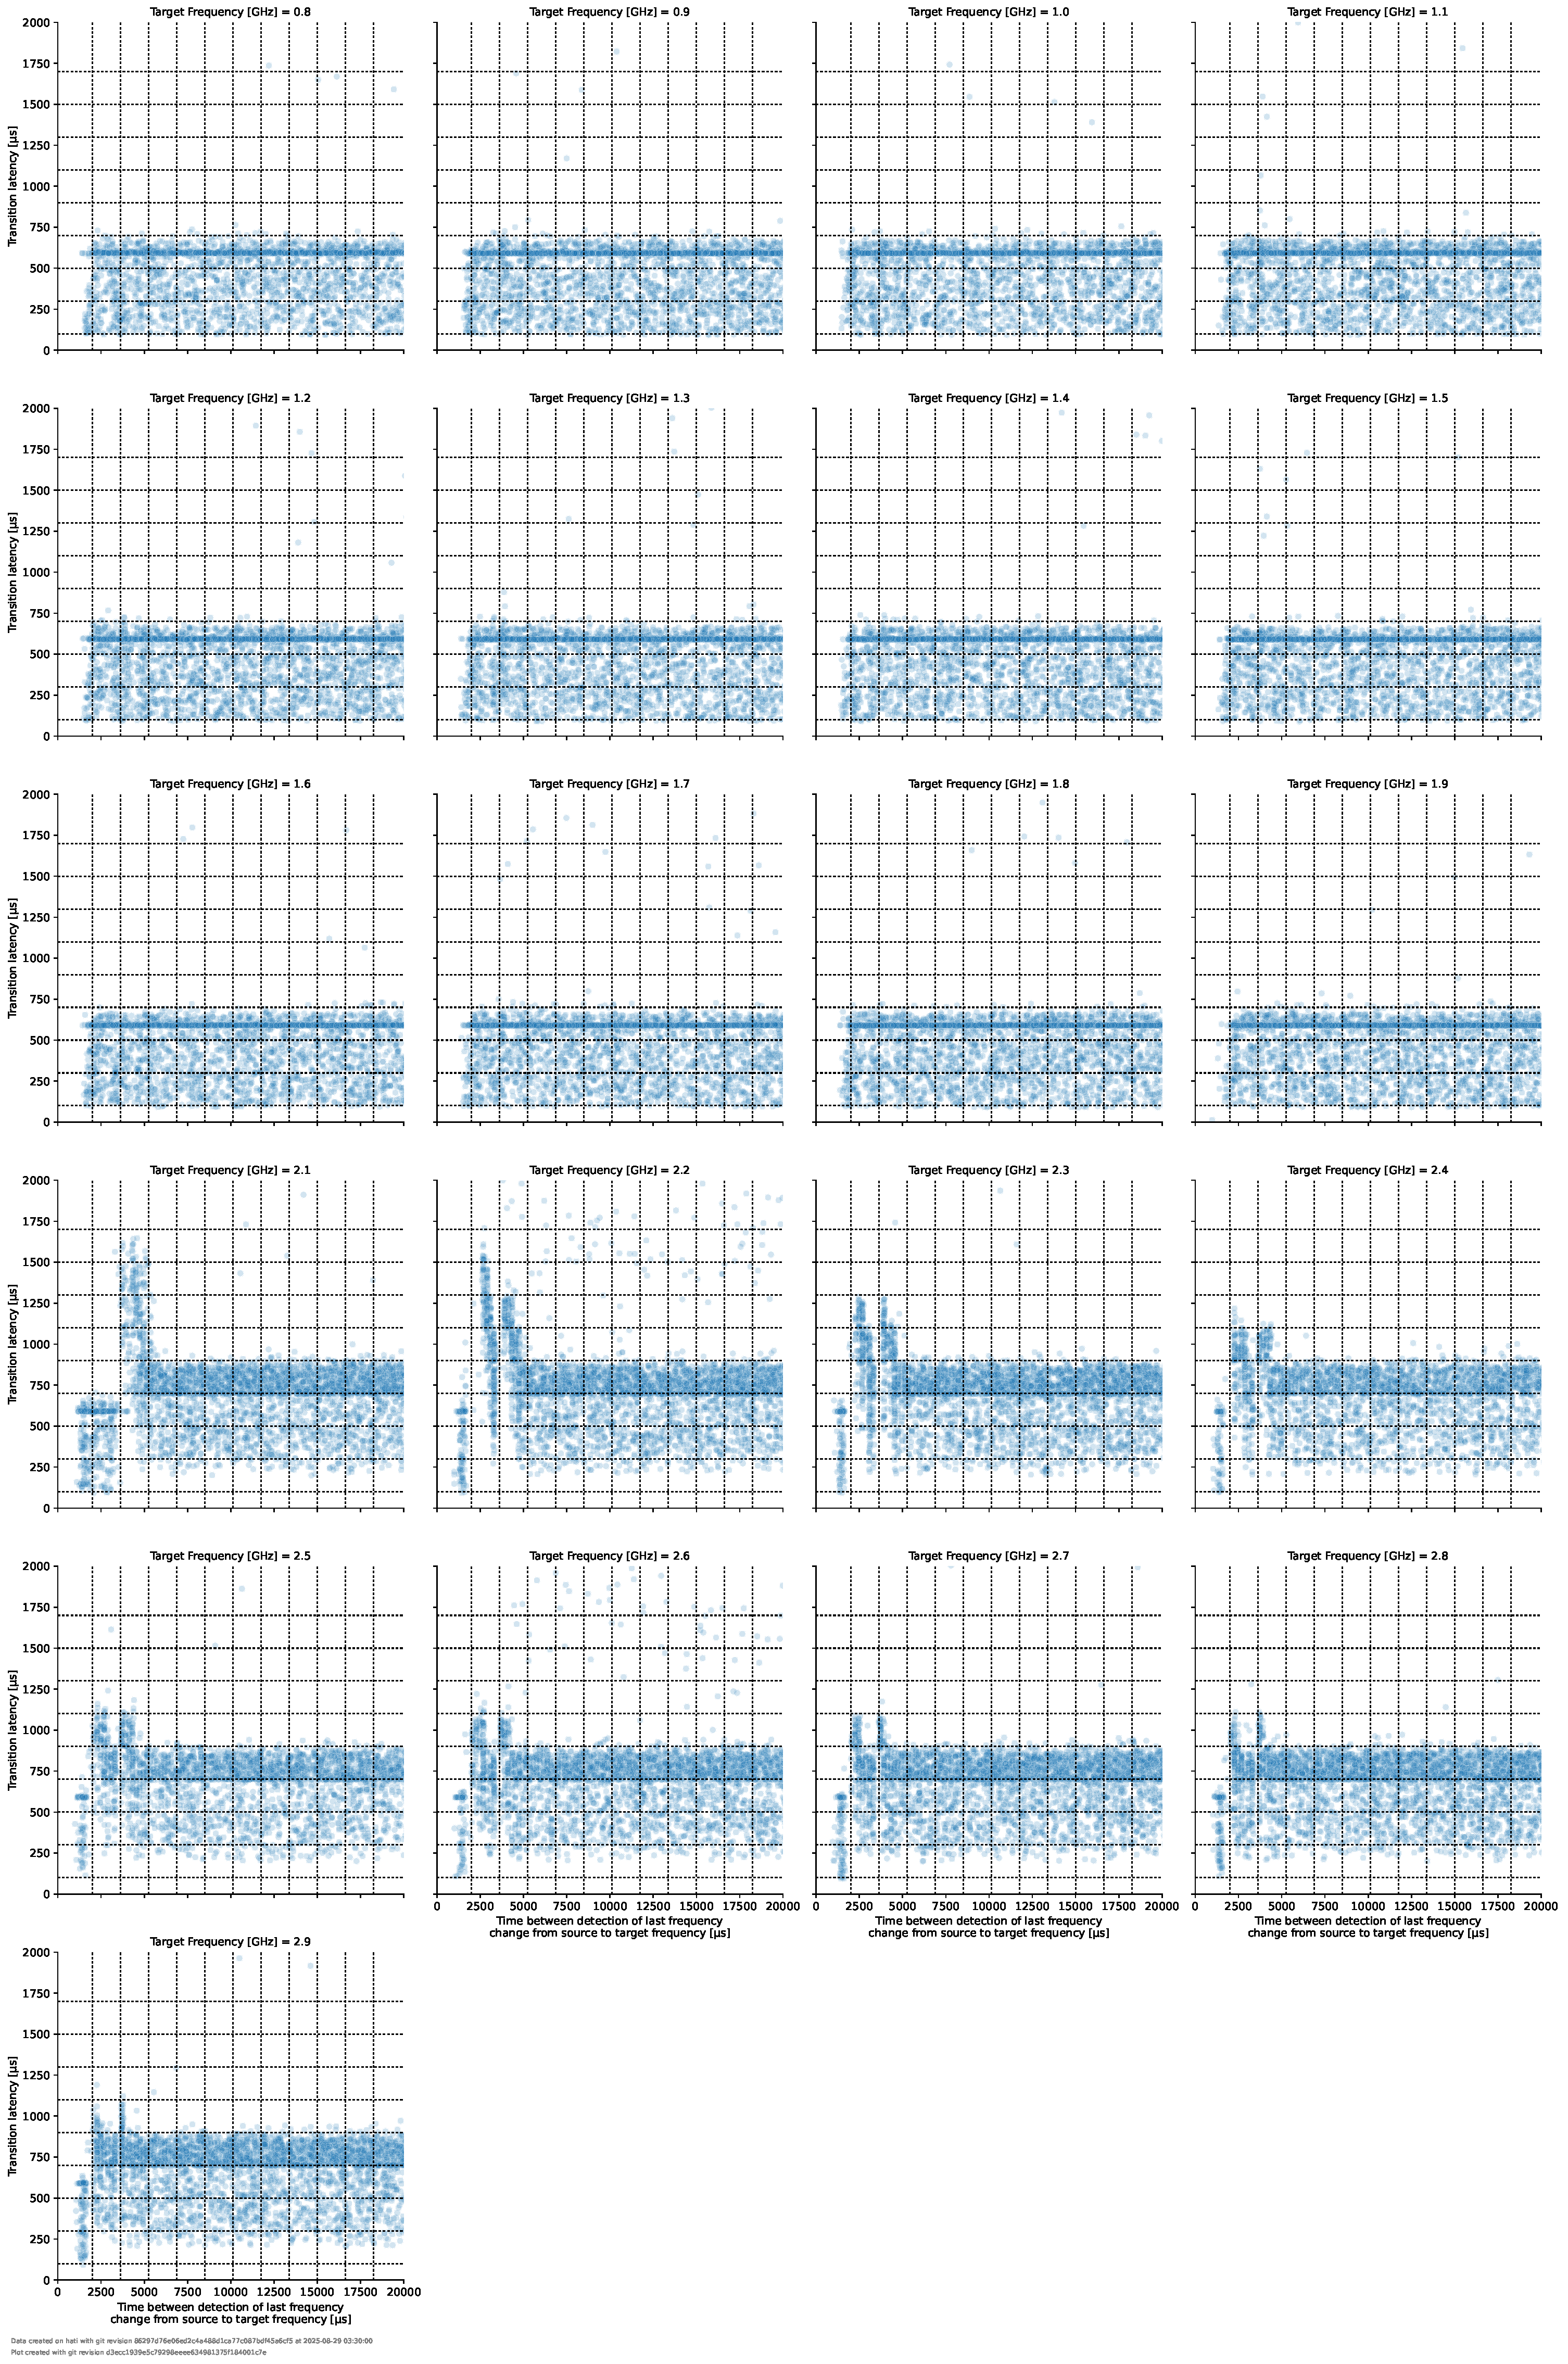
\includegraphics[width=\columnwidth]{fig/ftalat/ftalat_scatter_wait_transition_latency_hati_source_2.0.pdf}
    \caption{Dependance of the time between the detection events of transitions from \SI{2.0}{\GHz} to \SI{0.8}{}, \SI{0.9}{}, ..., \SI{2.9}{\GHz}. For better lines for bins of size \SI{1625}{\us} and \SI{200}{\us} have been included for the x and y-axis respectively.}
\end{figure}
\begin{figure}[]
    \centering
    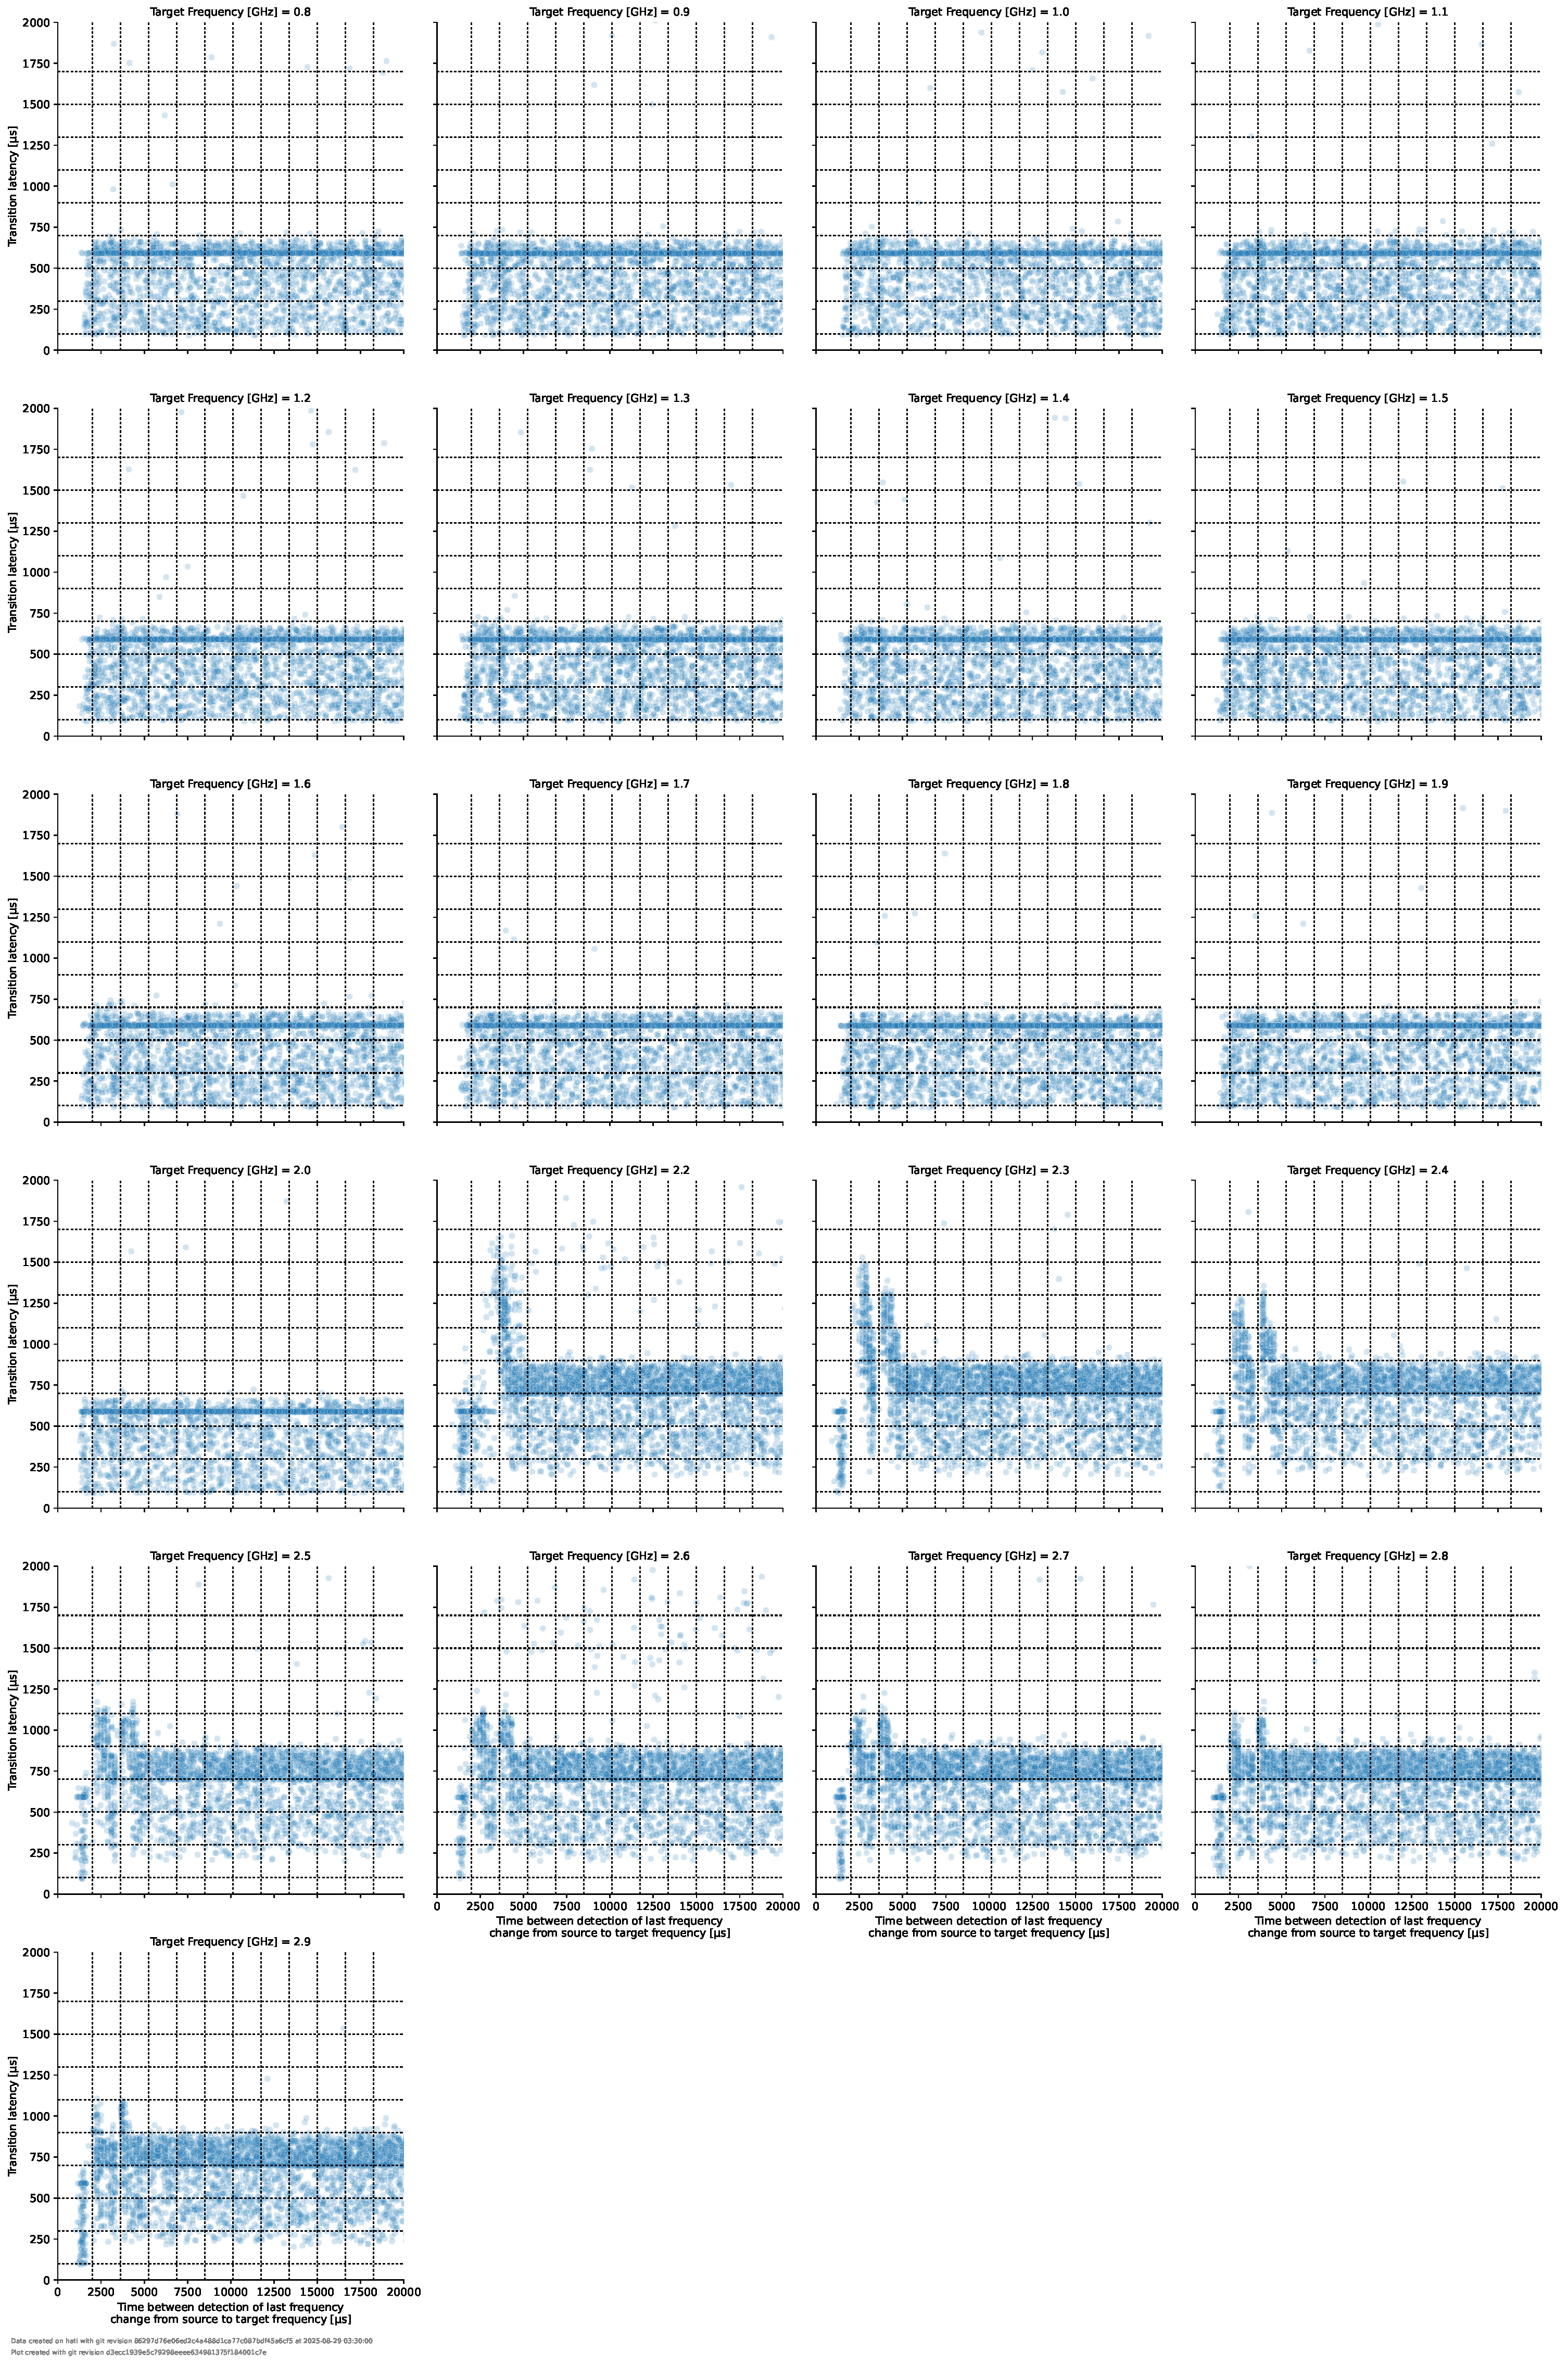
\includegraphics[width=\columnwidth]{fig/ftalat/ftalat_scatter_wait_transition_latency_hati_source_2.1.pdf}
    \caption{Dependance of the time between the detection events of transitions from \SI{2.1}{\GHz} to \SI{0.8}{}, \SI{0.9}{}, ..., \SI{2.9}{\GHz}. For better lines for bins of size \SI{1625}{\us} and \SI{200}{\us} have been included for the x and y-axis respectively.}
\end{figure}
\begin{figure}[]
    \centering
    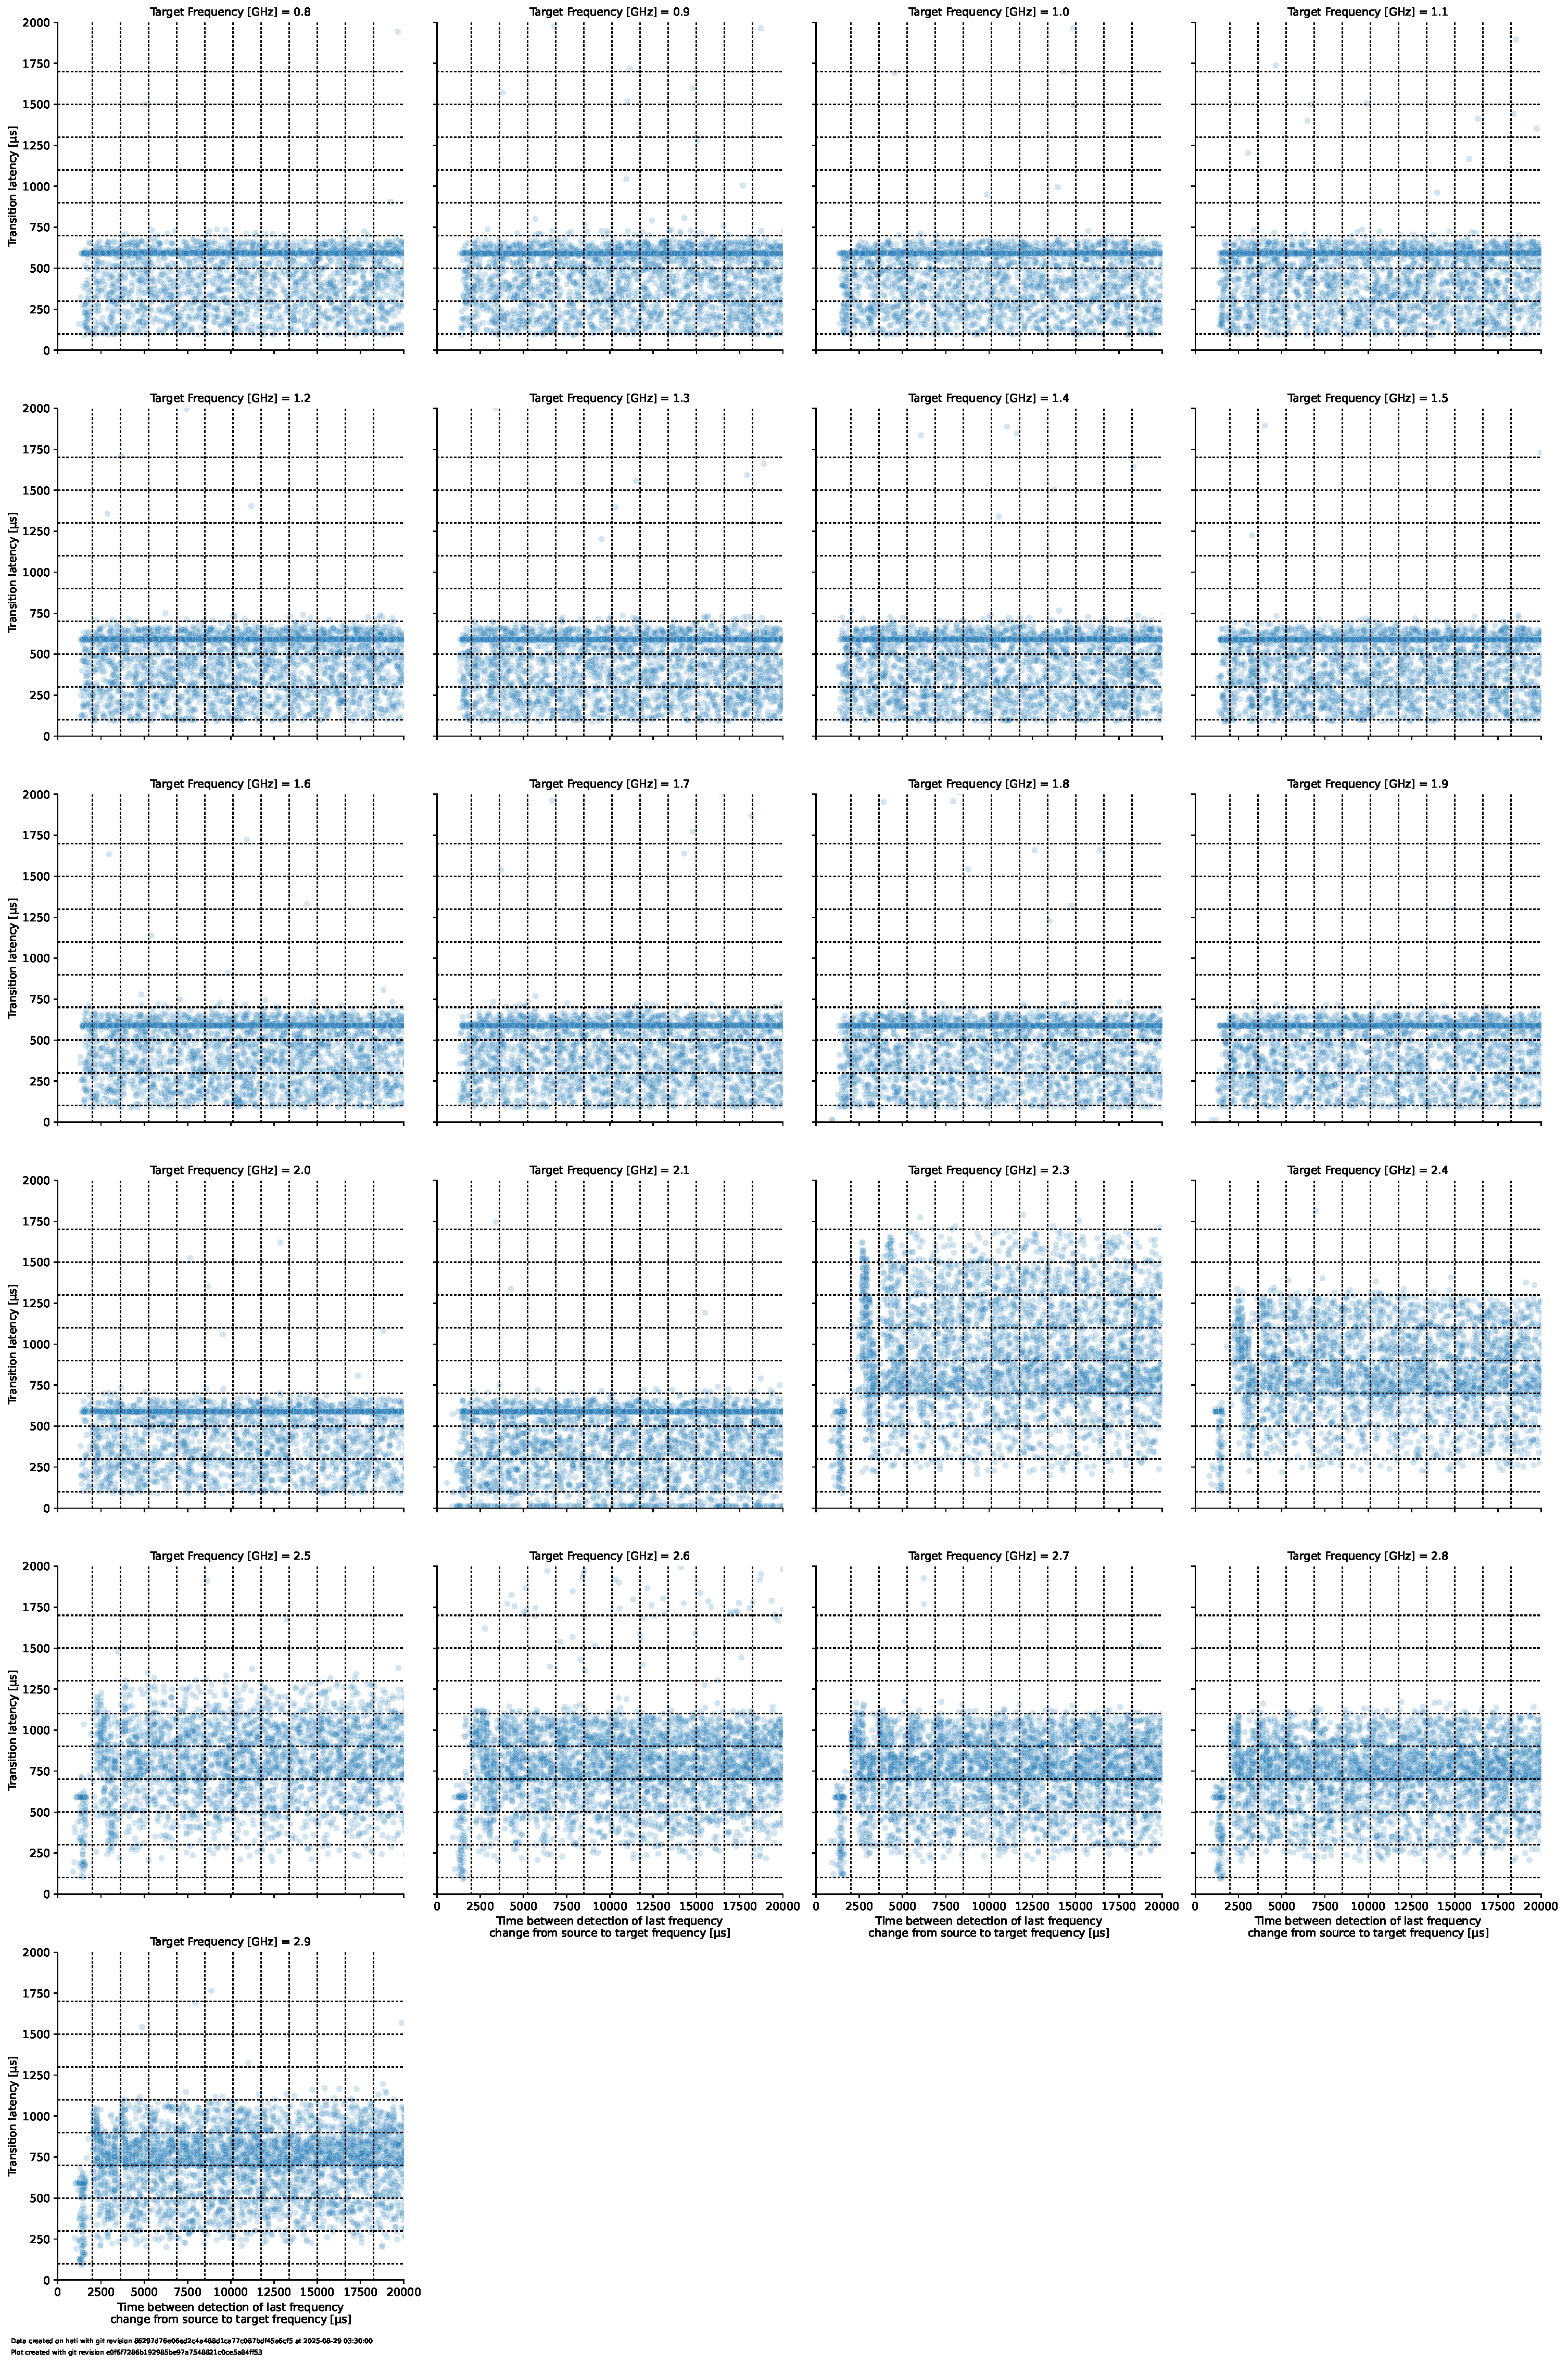
\includegraphics[width=\columnwidth]{fig/ftalat/ftalat_scatter_wait_transition_latency_hati_source_2.2.pdf}
    \caption{Dependance of the time between the detection events of transitions from \SI{2.2}{\GHz} to \SI{0.8}{}, \SI{0.9}{}, ..., \SI{2.9}{\GHz}. For better lines for bins of size \SI{1625}{\us} and \SI{200}{\us} have been included for the x and y-axis respectively.}
\end{figure}
\begin{figure}[]
    \centering
    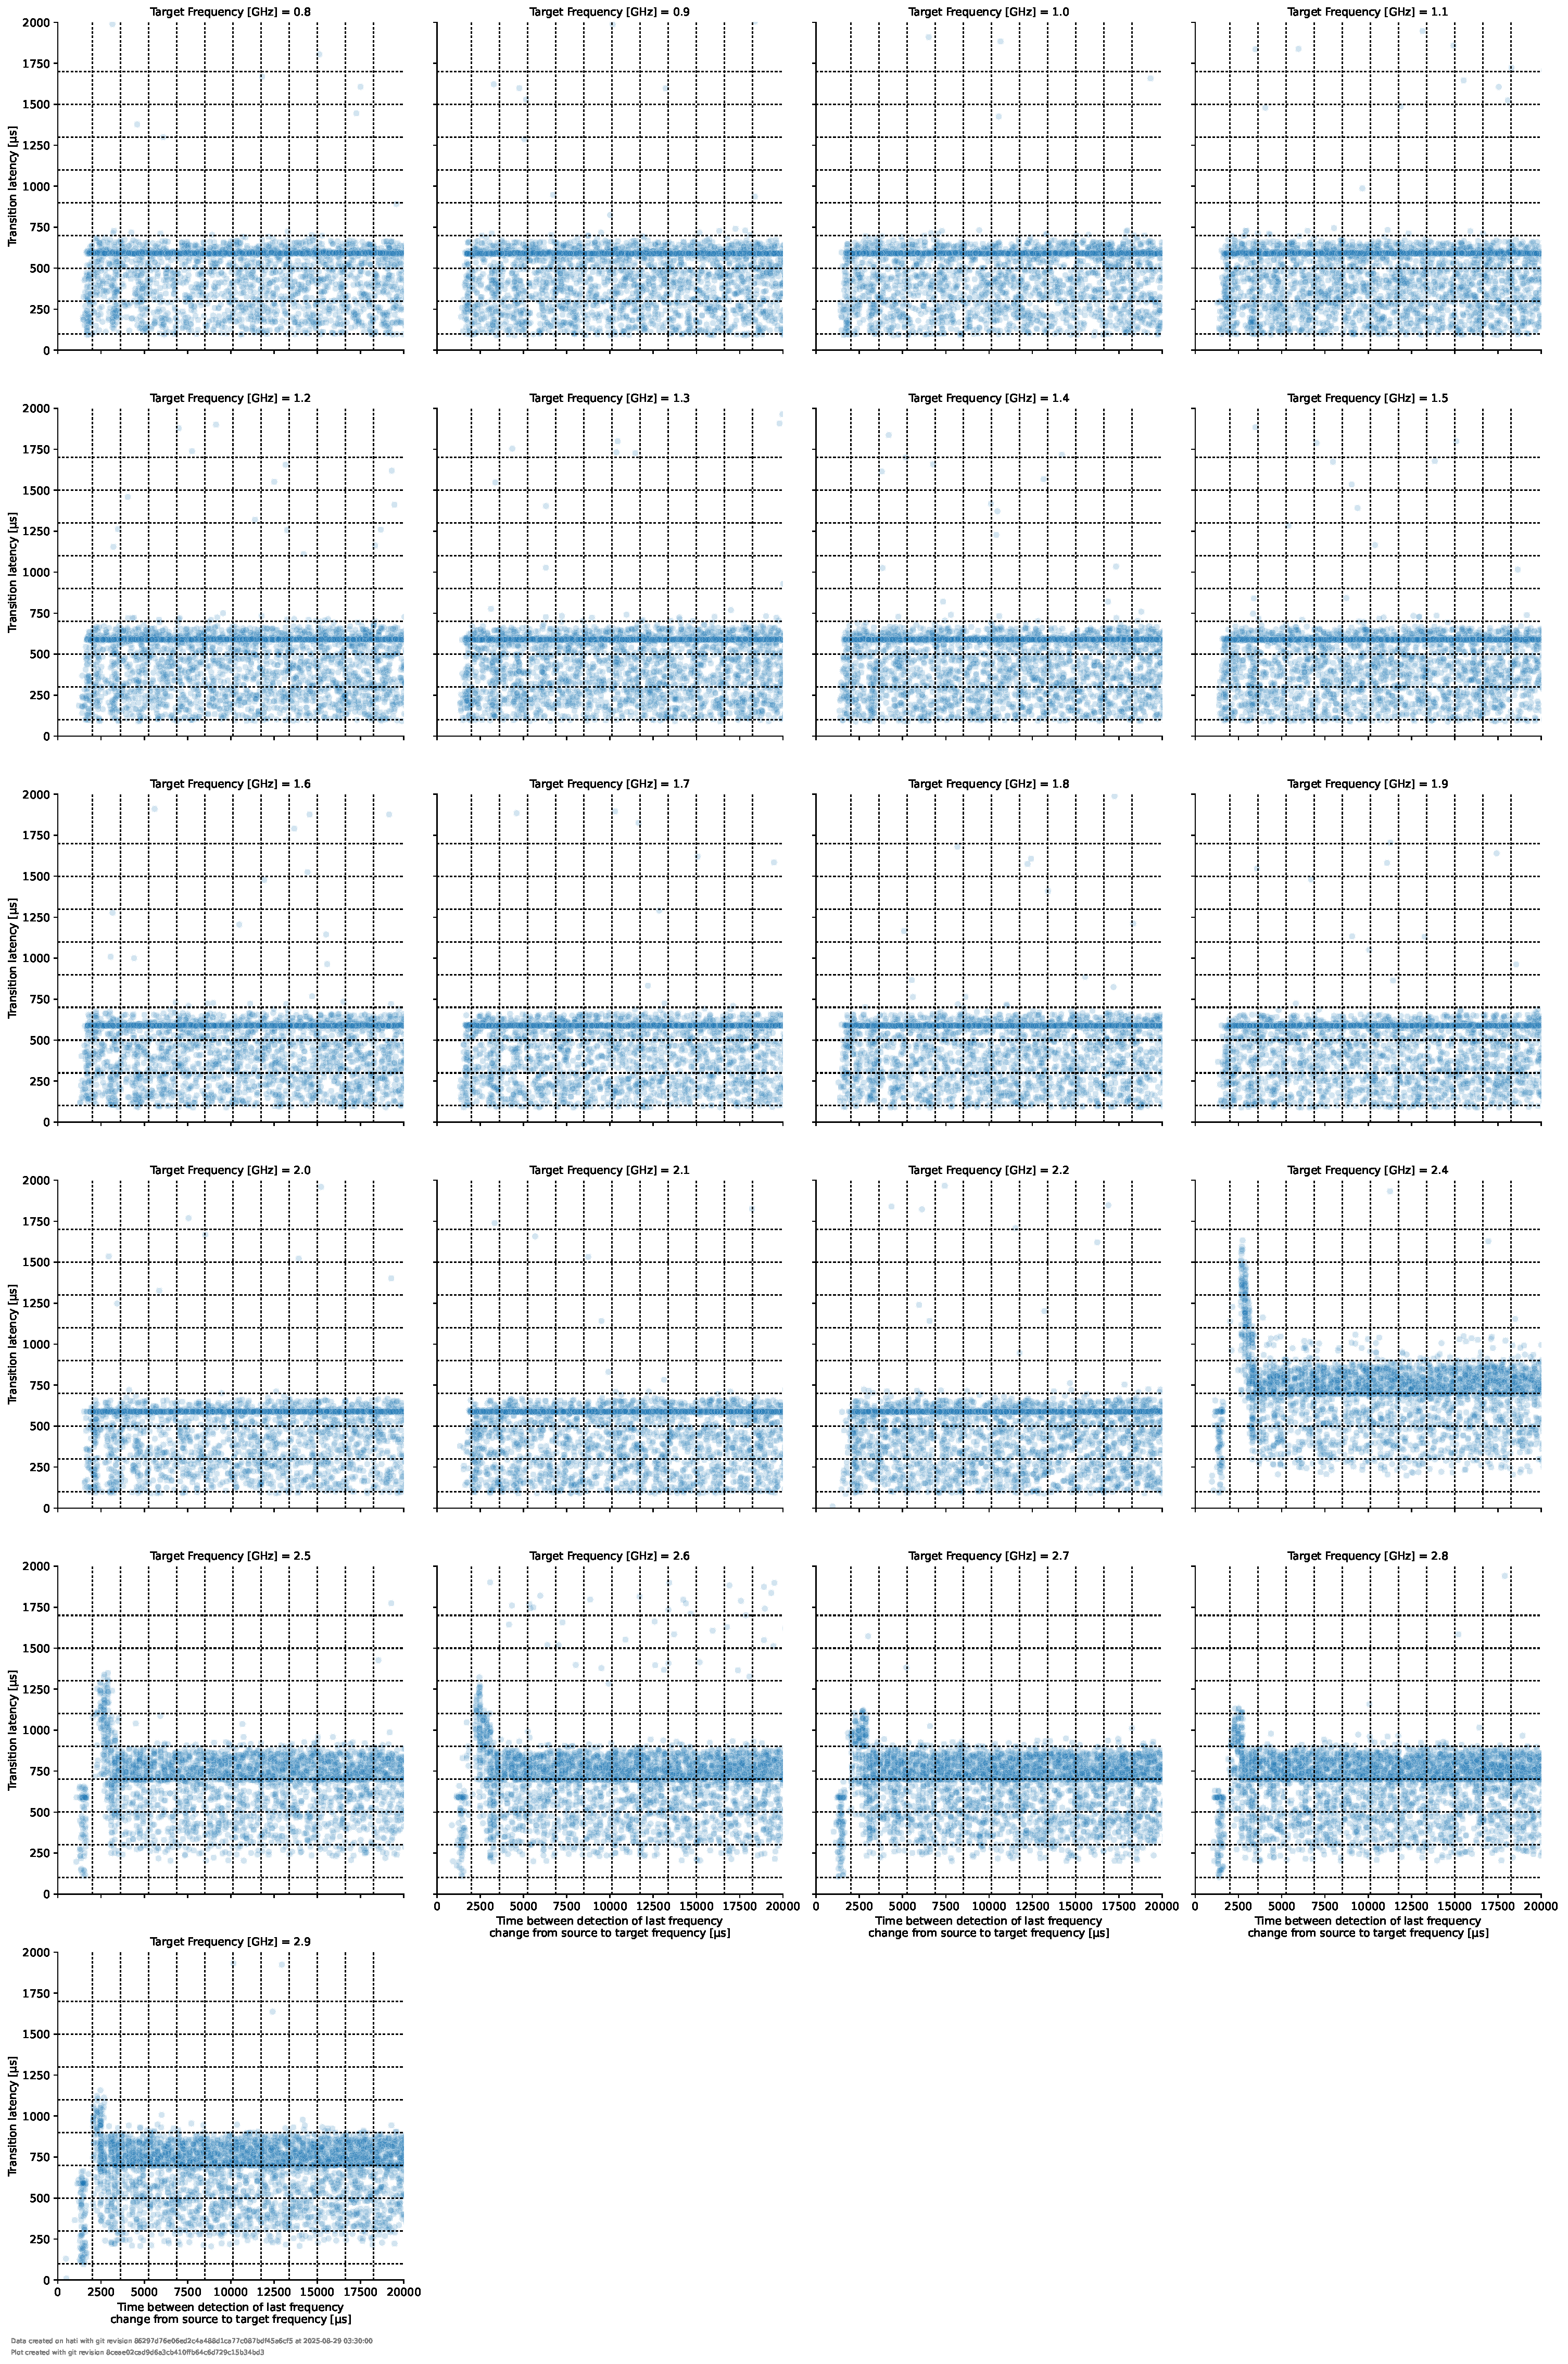
\includegraphics[width=\columnwidth]{fig/ftalat/ftalat_scatter_wait_transition_latency_hati_source_2.3.pdf}
    \caption{Dependance of the time between the detection events of transitions from \SI{2.3}{\GHz} to \SI{0.8}{}, \SI{0.9}{}, ..., \SI{2.9}{\GHz}. For better lines for bins of size \SI{1625}{\us} and \SI{200}{\us} have been included for the x and y-axis respectively.}
\end{figure}
\begin{figure}[]
    \centering
    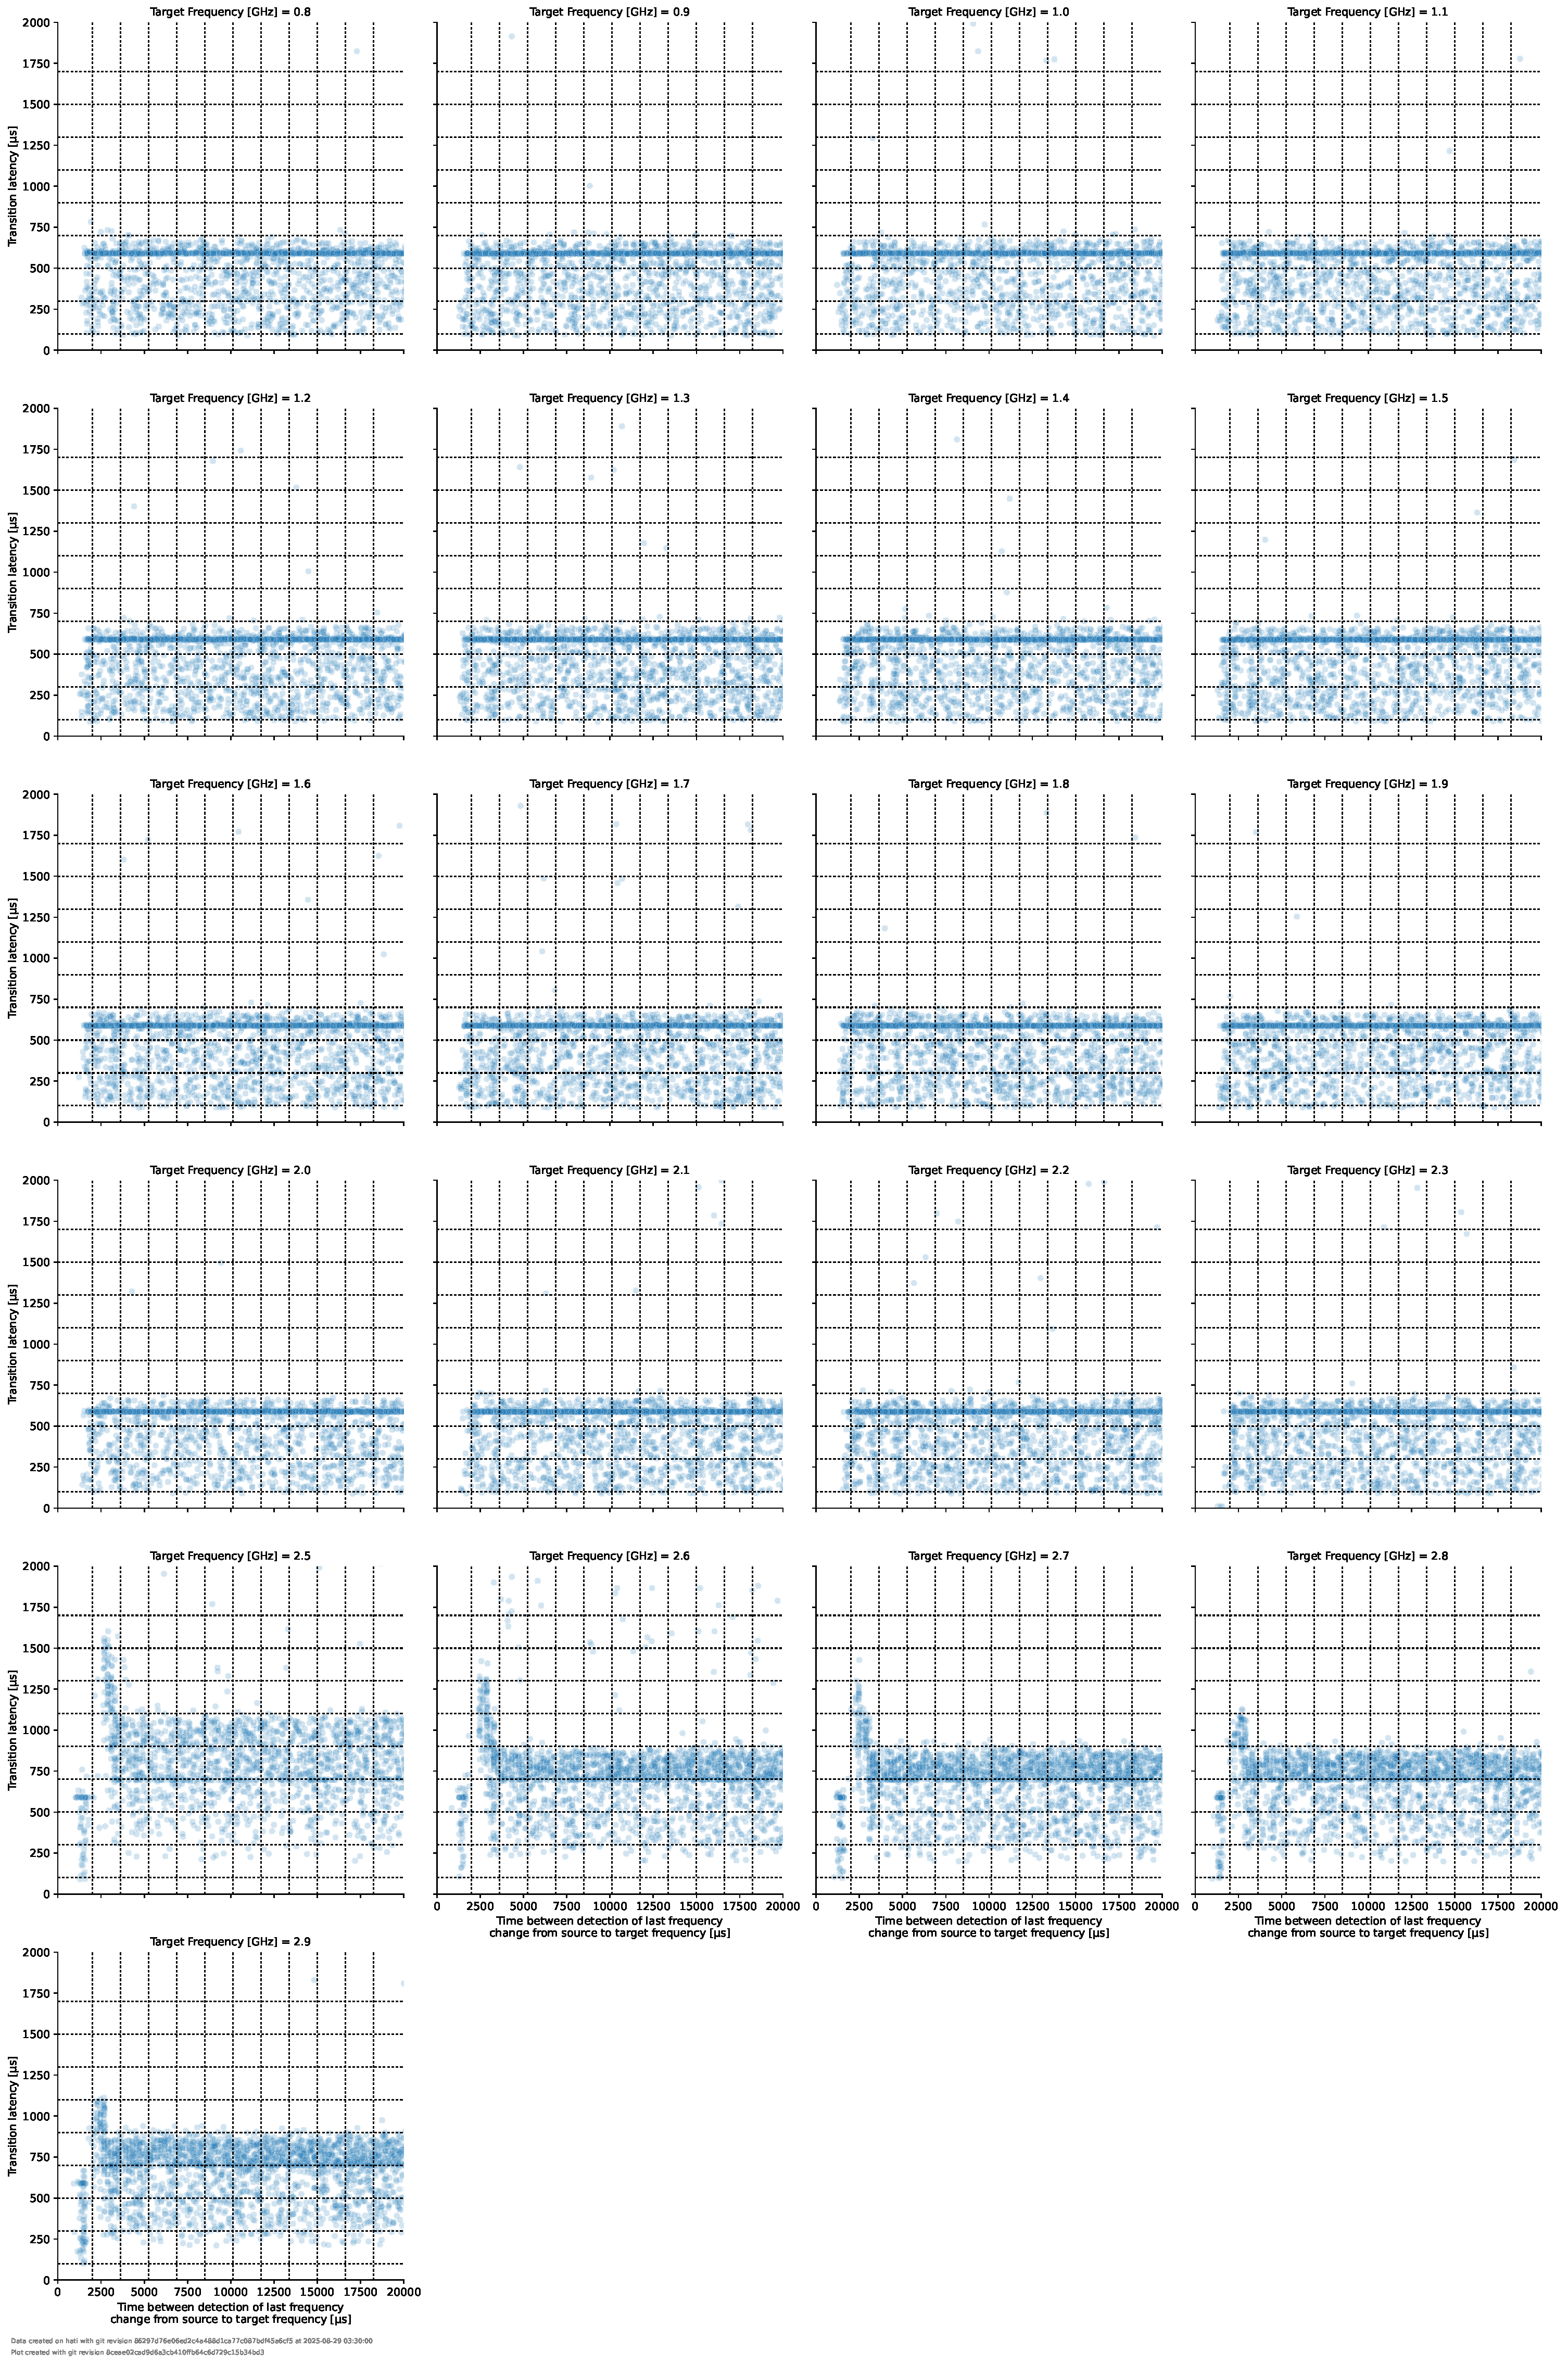
\includegraphics[width=\columnwidth]{fig/ftalat/ftalat_scatter_wait_transition_latency_hati_source_2.4.pdf}
    \caption{Dependance of the time between the detection events of transitions from \SI{2.4}{\GHz} to \SI{0.8}{}, \SI{0.9}{}, ..., \SI{2.9}{\GHz}. For better lines for bins of size \SI{1625}{\us} and \SI{200}{\us} have been included for the x and y-axis respectively.}
\end{figure}
\begin{figure}[]
    \centering
    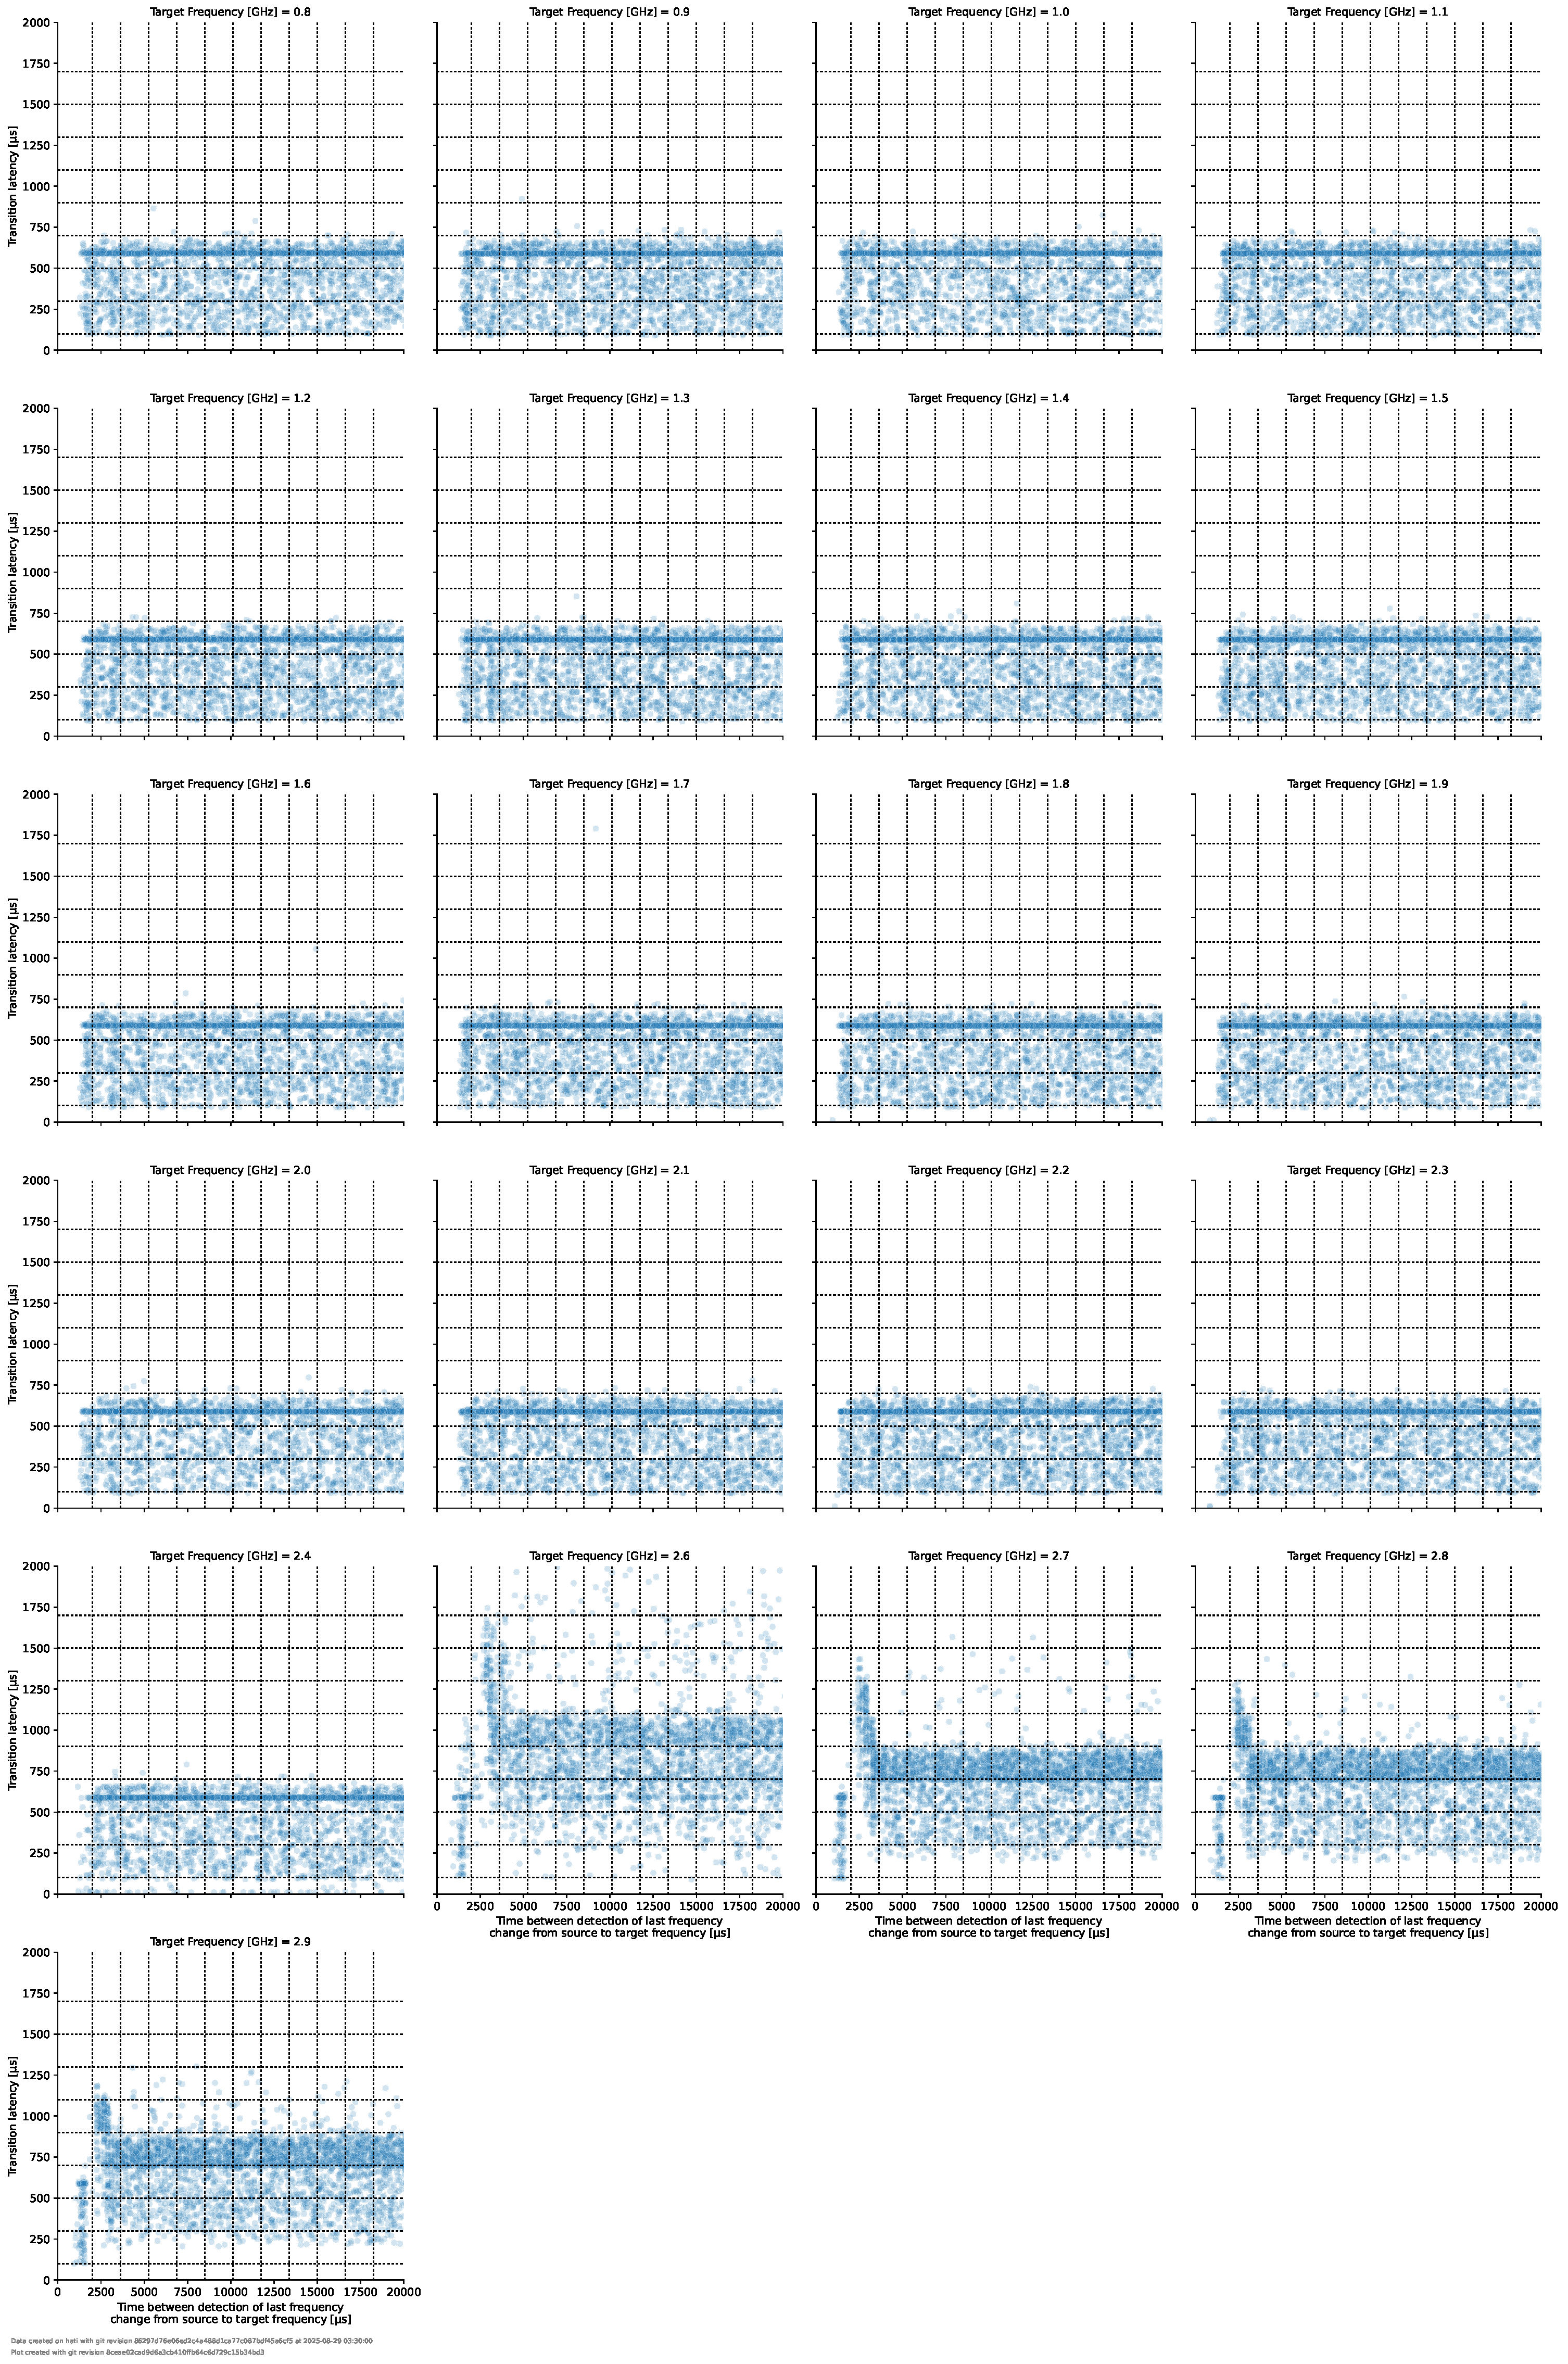
\includegraphics[width=\columnwidth]{fig/ftalat/ftalat_scatter_wait_transition_latency_hati_source_2.5.pdf}
    \caption{Dependance of the time between the detection events of transitions from \SI{2.5}{\GHz} to \SI{0.8}{}, \SI{0.9}{}, ..., \SI{2.9}{\GHz}. For better lines for bins of size \SI{1625}{\us} and \SI{200}{\us} have been included for the x and y-axis respectively.}
\end{figure}
\begin{figure}[]
    \centering
    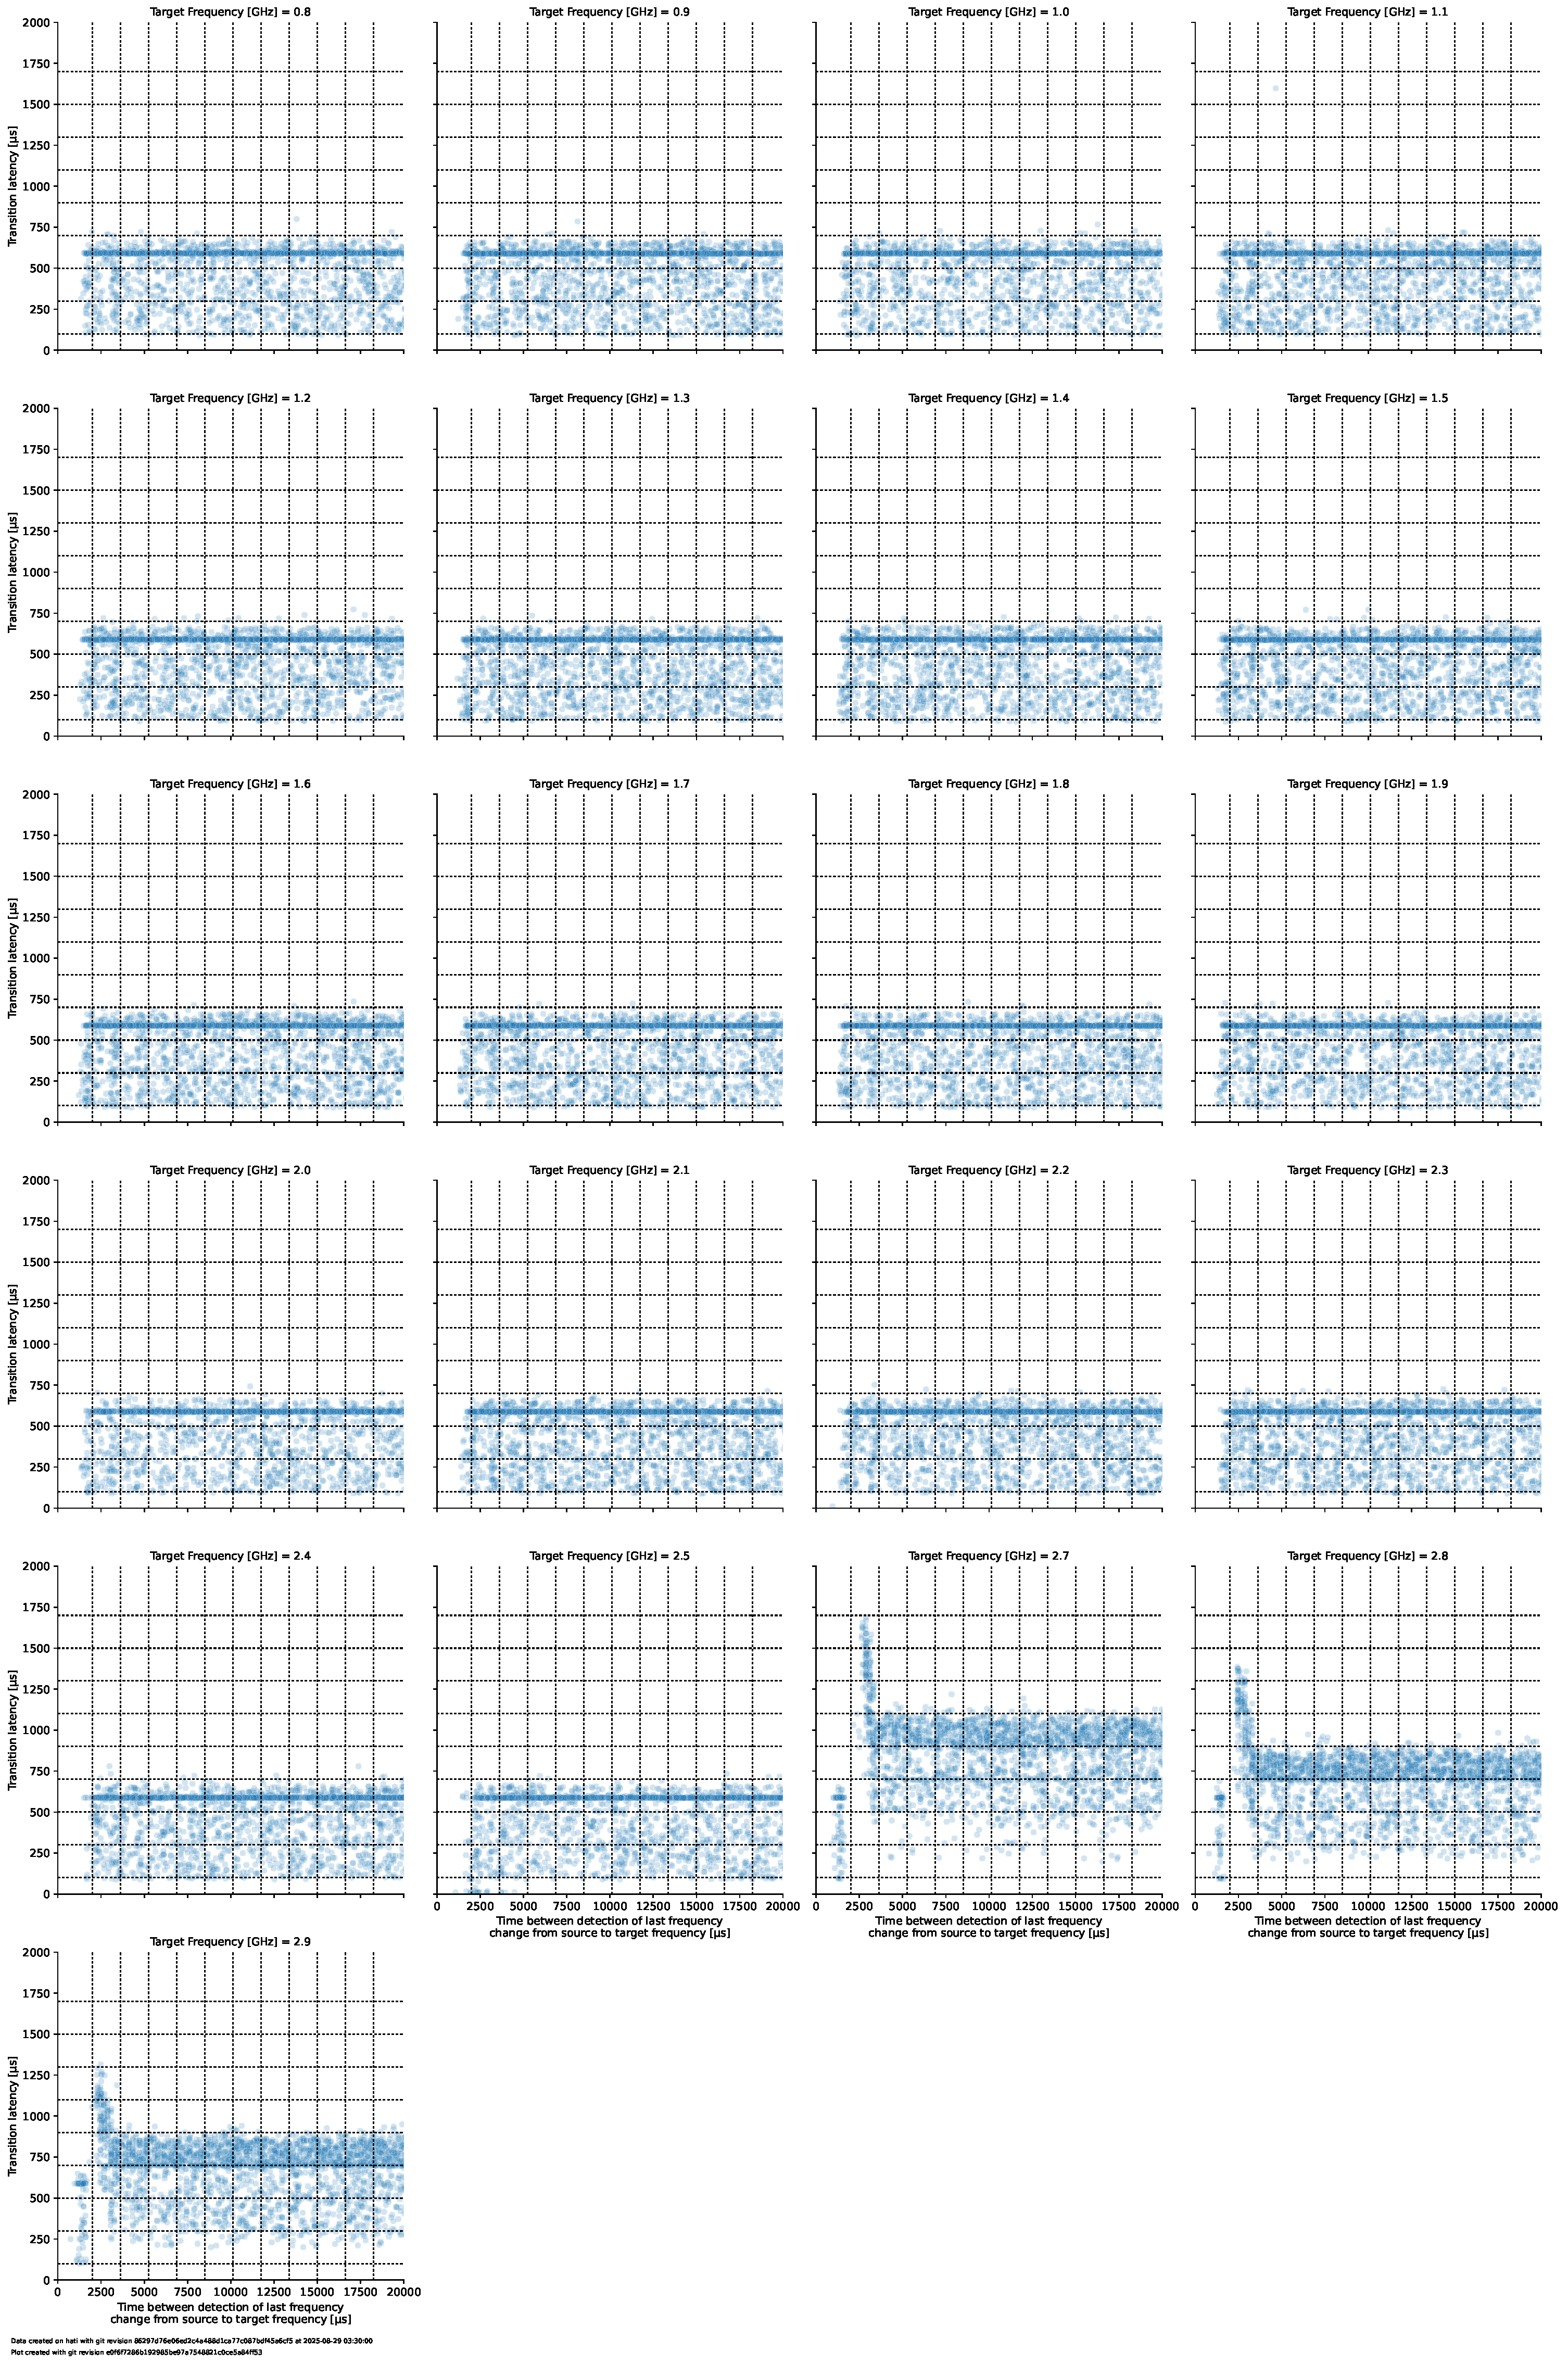
\includegraphics[width=\columnwidth]{fig/ftalat/ftalat_scatter_wait_transition_latency_hati_source_2.6.pdf}
    \caption{Dependance of the time between the detection events of transitions from \SI{2.6}{\GHz} to \SI{0.8}{}, \SI{0.9}{}, ..., \SI{2.9}{\GHz}. For better lines for bins of size \SI{1625}{\us} and \SI{200}{\us} have been included for the x and y-axis respectively.}
\end{figure}
\begin{figure}[]
    \centering
    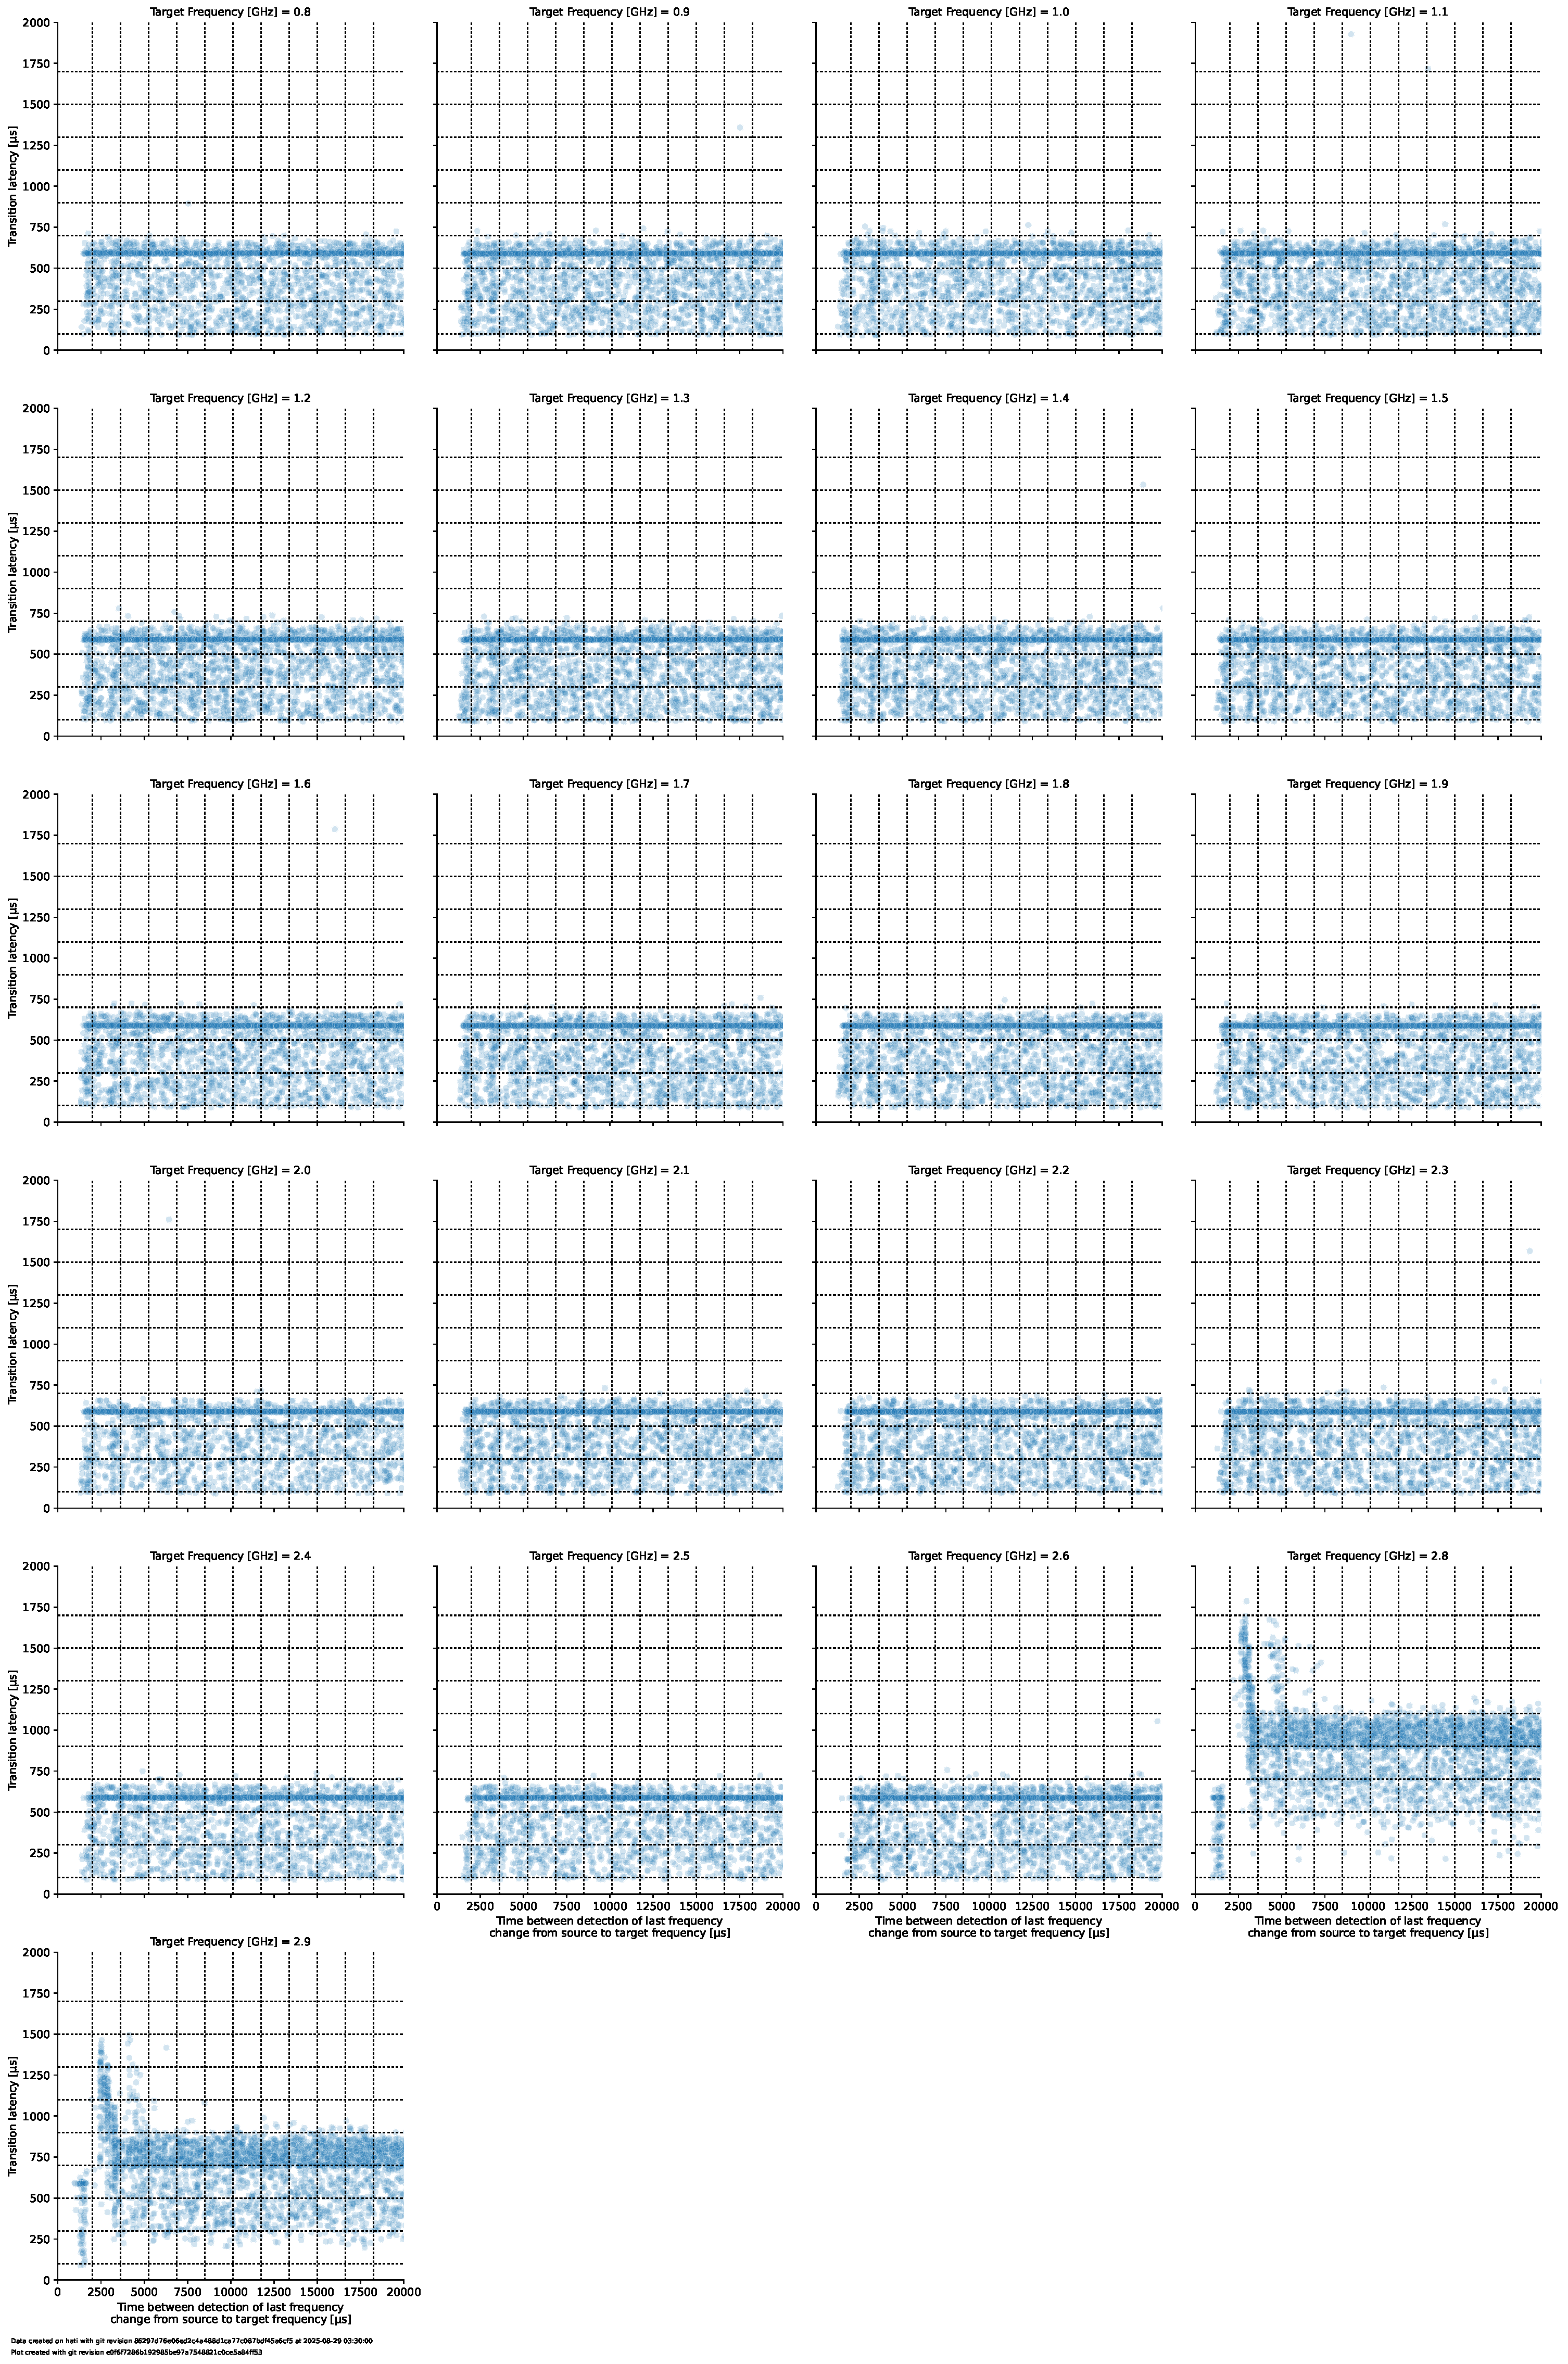
\includegraphics[width=\columnwidth]{fig/ftalat/ftalat_scatter_wait_transition_latency_hati_source_2.7.pdf}
    \caption{Dependance of the time between the detection events of transitions from \SI{2.7}{\GHz} to \SI{0.8}{}, \SI{0.9}{}, ..., \SI{2.9}{\GHz}. For better lines for bins of size \SI{1625}{\us} and \SI{200}{\us} have been included for the x and y-axis respectively.}
\end{figure}
\begin{figure}[]
    \centering
    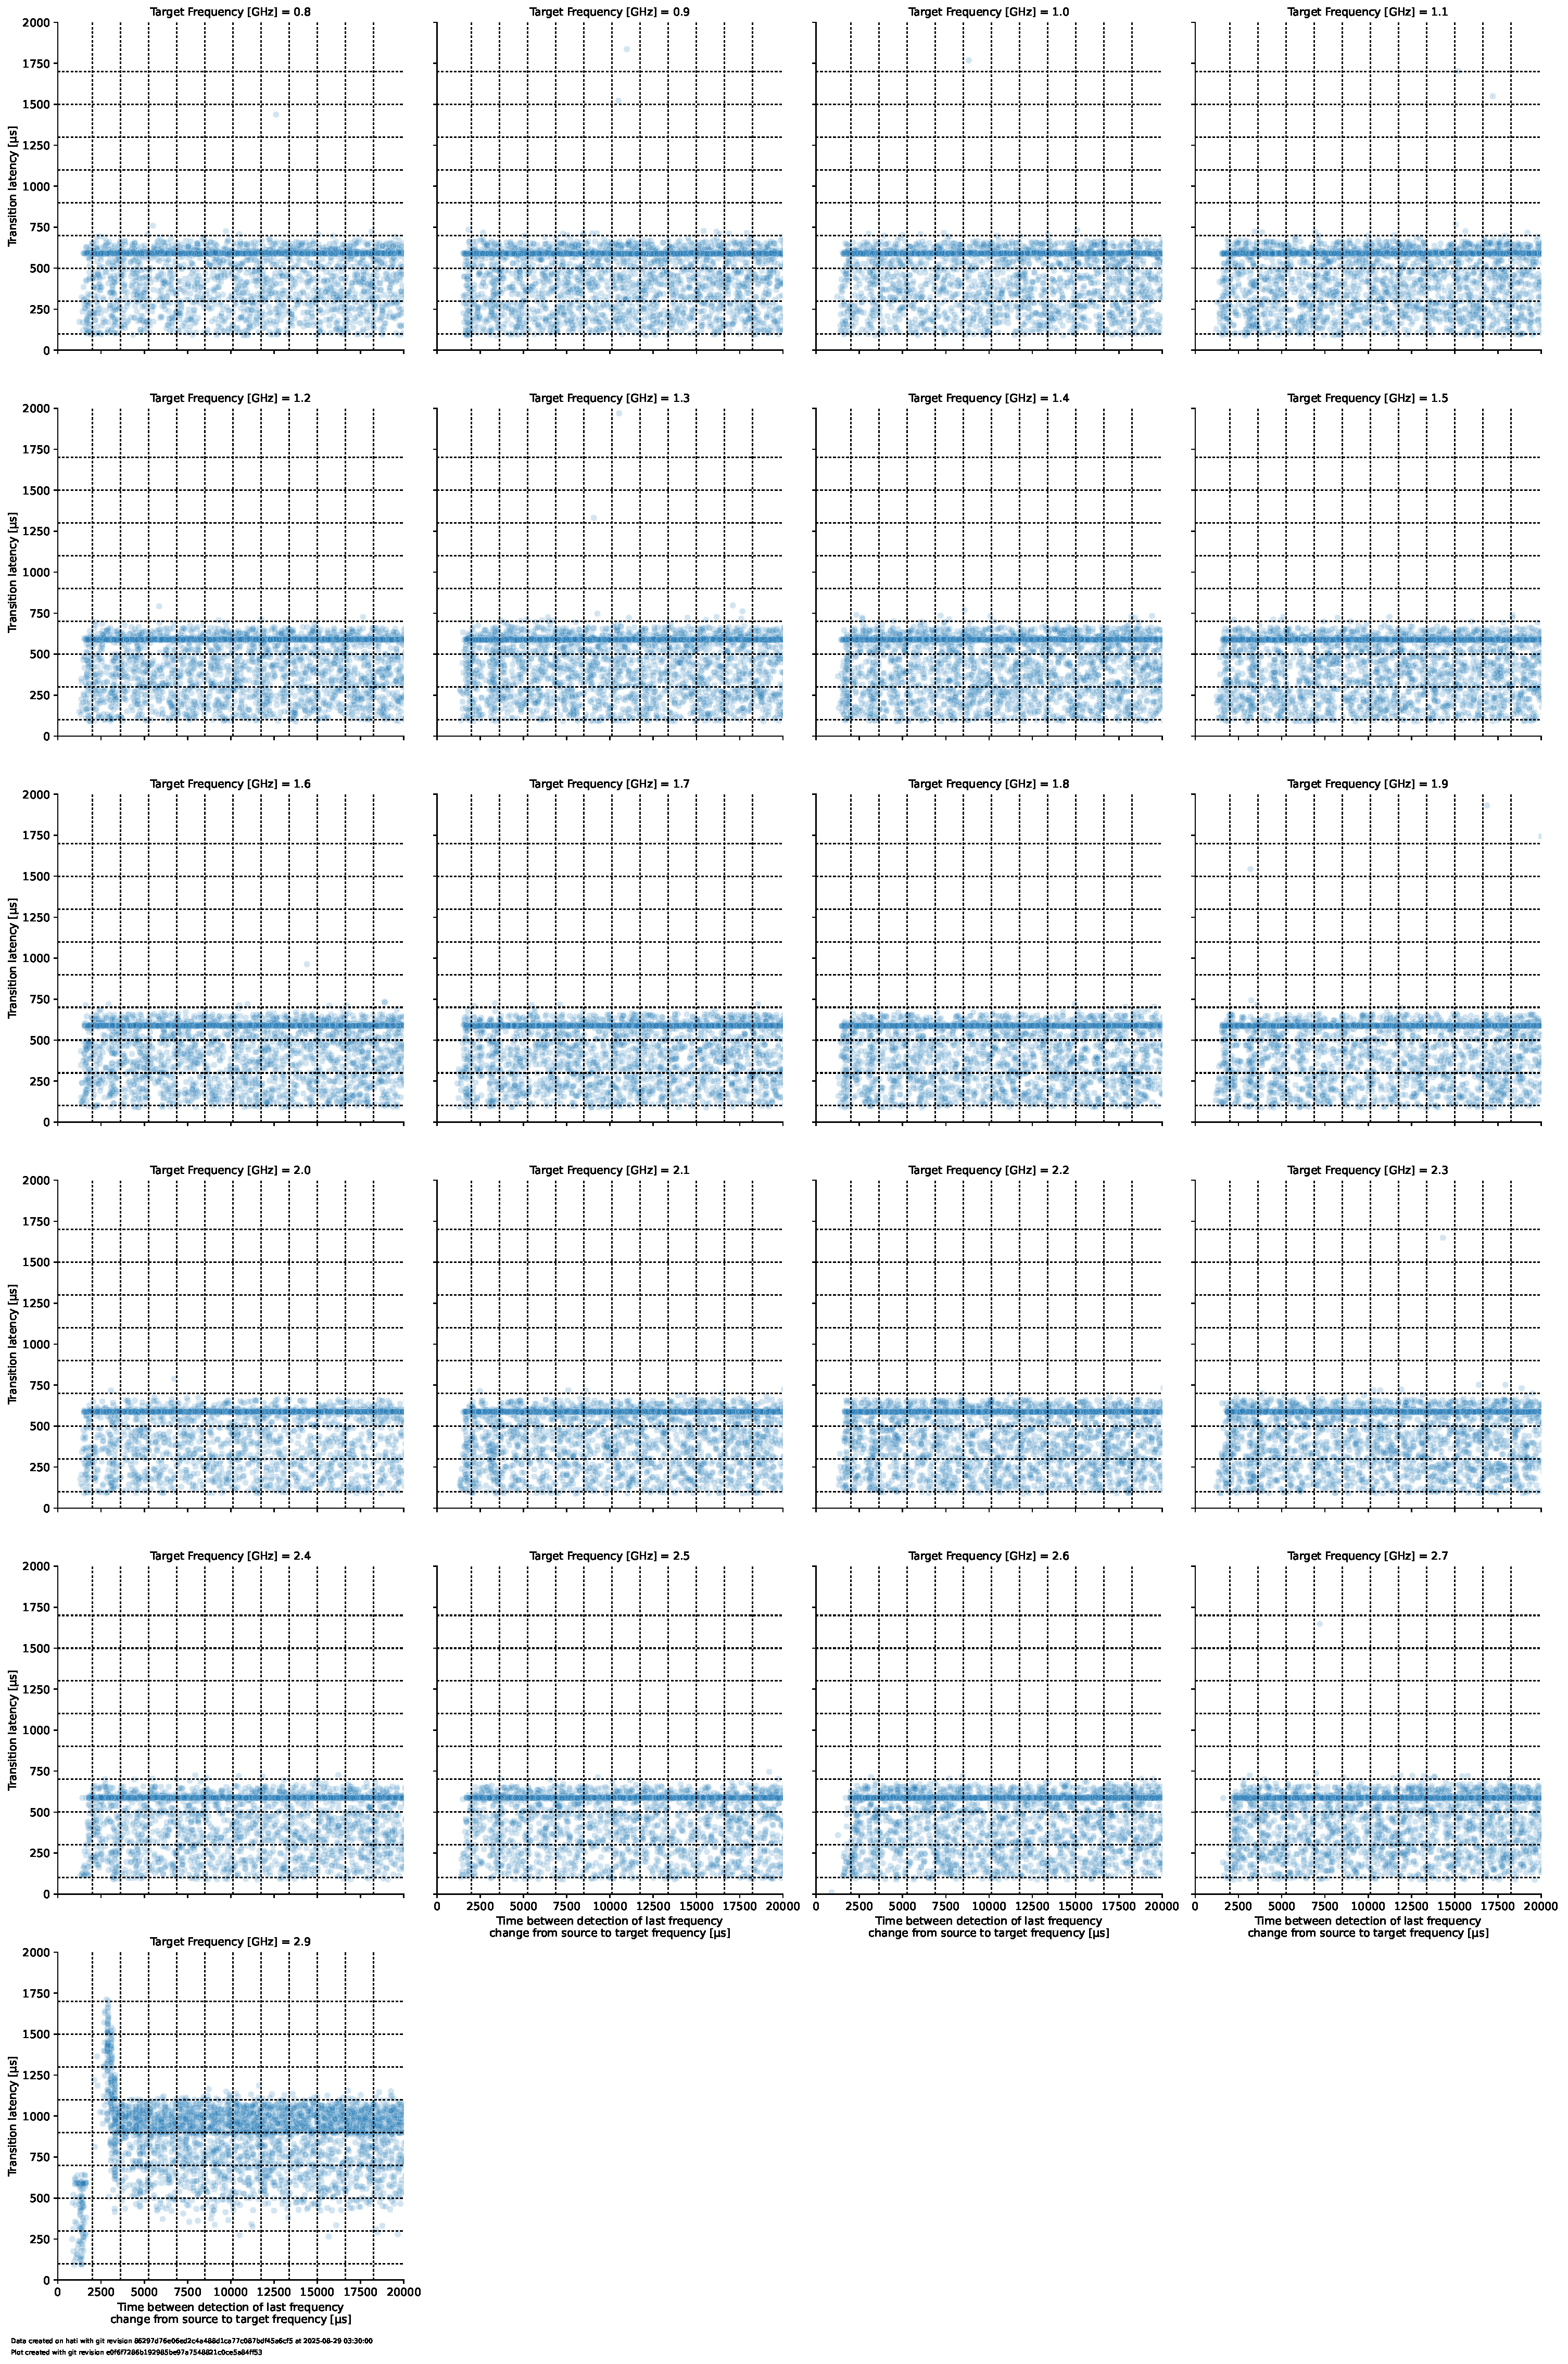
\includegraphics[width=\columnwidth]{fig/ftalat/ftalat_scatter_wait_transition_latency_hati_source_2.8.pdf}
    \caption{Dependance of the time between the detection events of transitions from \SI{2.8}{\GHz} to \SI{0.8}{}, \SI{0.9}{}, ..., \SI{2.9}{\GHz}. For better lines for bins of size \SI{1625}{\us} and \SI{200}{\us} have been included for the x and y-axis respectively.}
\end{figure}
\begin{figure}[]
    \centering
    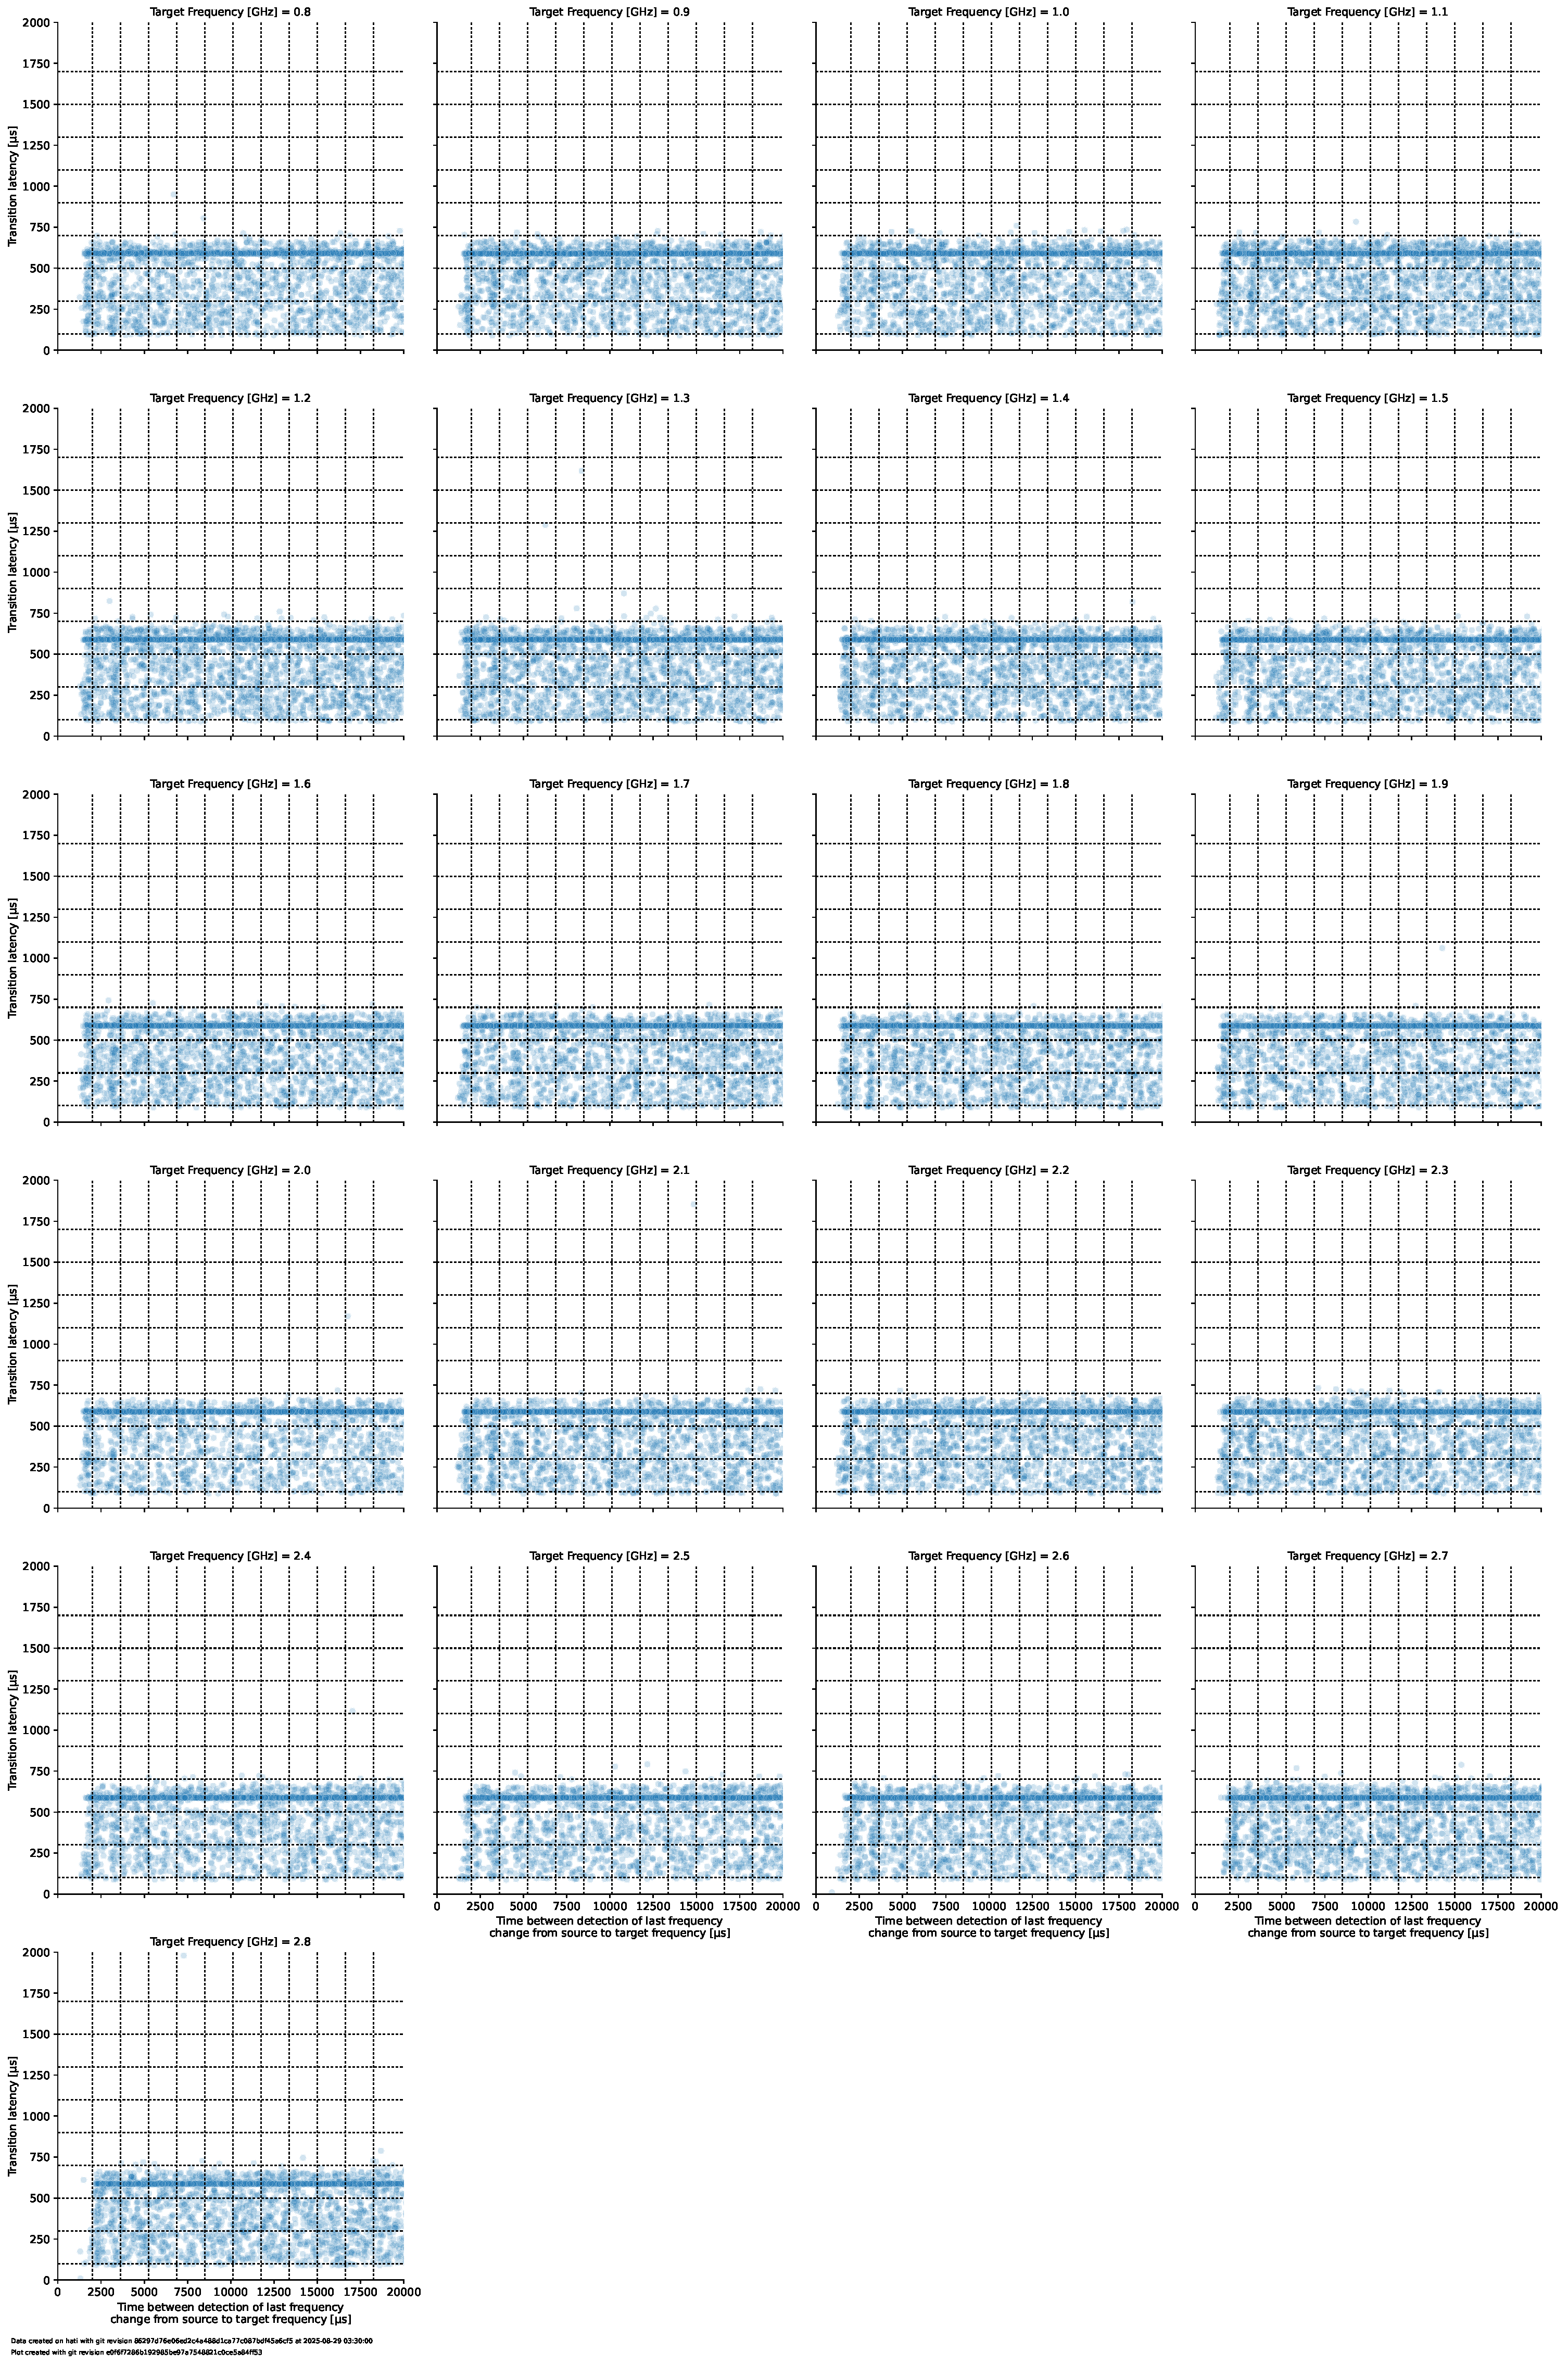
\includegraphics[width=\columnwidth]{fig/ftalat/ftalat_scatter_wait_transition_latency_hati_source_2.9.pdf}
    \caption{Dependance of the time between the detection events of transitions from \SI{2.9}{\GHz} to \SI{0.8}{}, \SI{0.9}{}, ..., \SI{2.9}{\GHz}. For better lines for bins of size \SI{1625}{\us} and \SI{200}{\us} have been included for the x and y-axis respectively.}
\end{figure}

\chapter{Appendix Core to Core Communication Latencies}
\label{app:core_to_core_latencies_complete}
This section includes all scatter plots for all measurements conducted with the core to core communication latency benchmark as described in~\secref{TODO}.

\begin{figure}[]
    \centering
    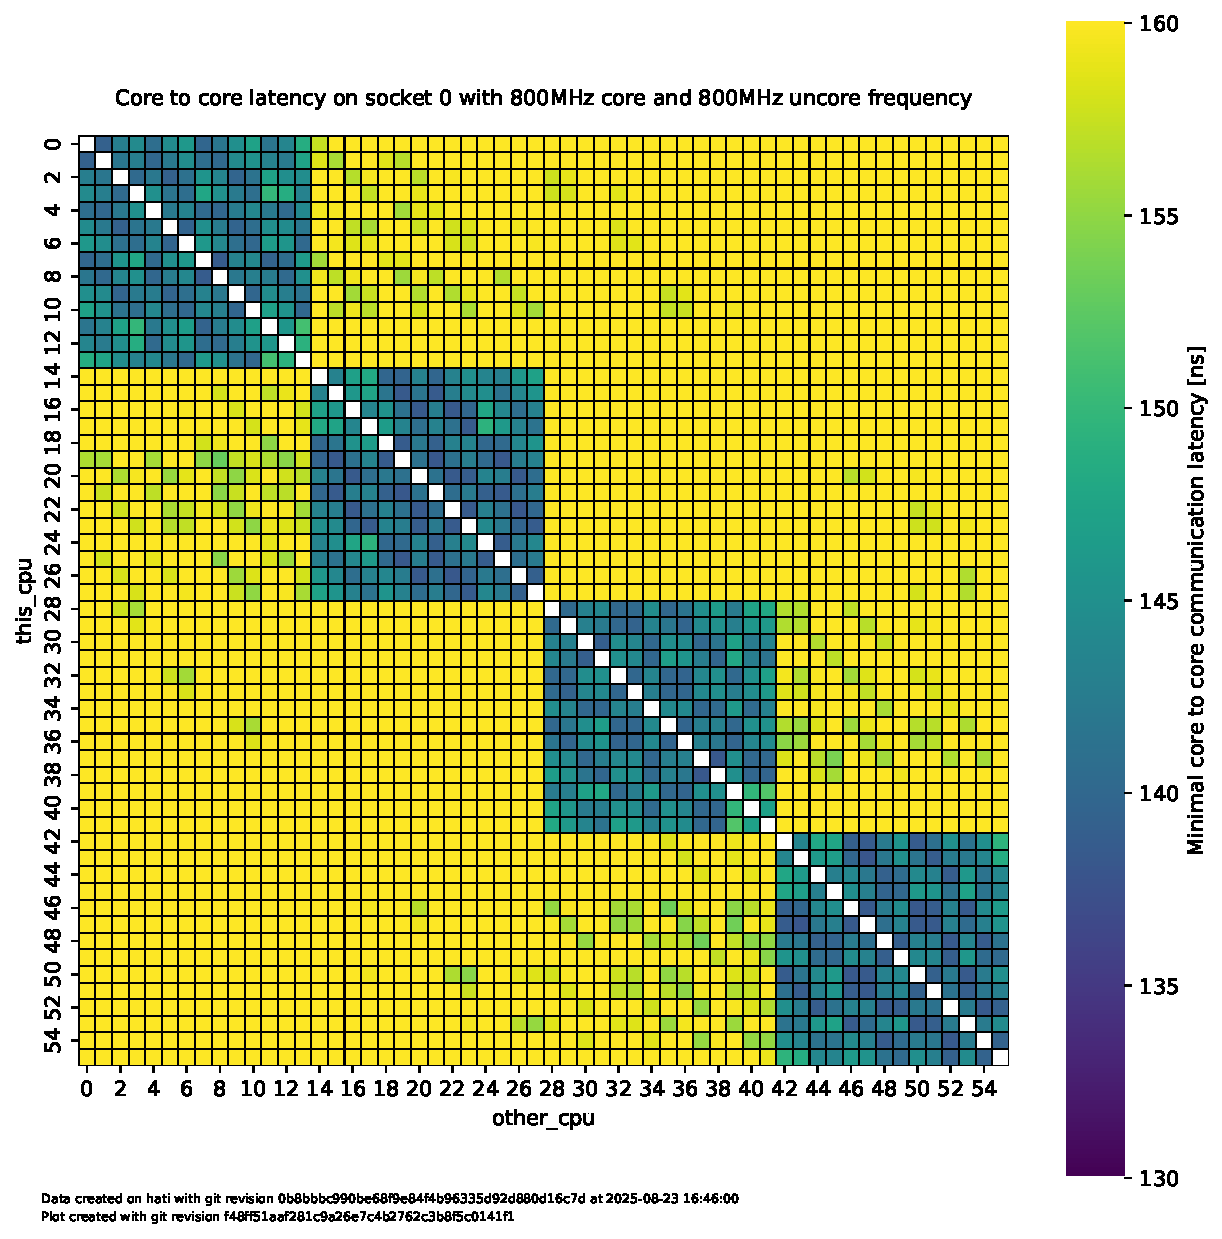
\includegraphics[width=\columnwidth]{fig/core-to-core-latency/core-to-core-heatmap-min-800-800.pdf}
    \caption{Minimal core to core communication latency for hati's socket 0 with \SI{0.8}{\GHz} core and \SI{0.8}{\GHz} uncore frequency.}
\end{figure}
\begin{figure}[]
    \centering
    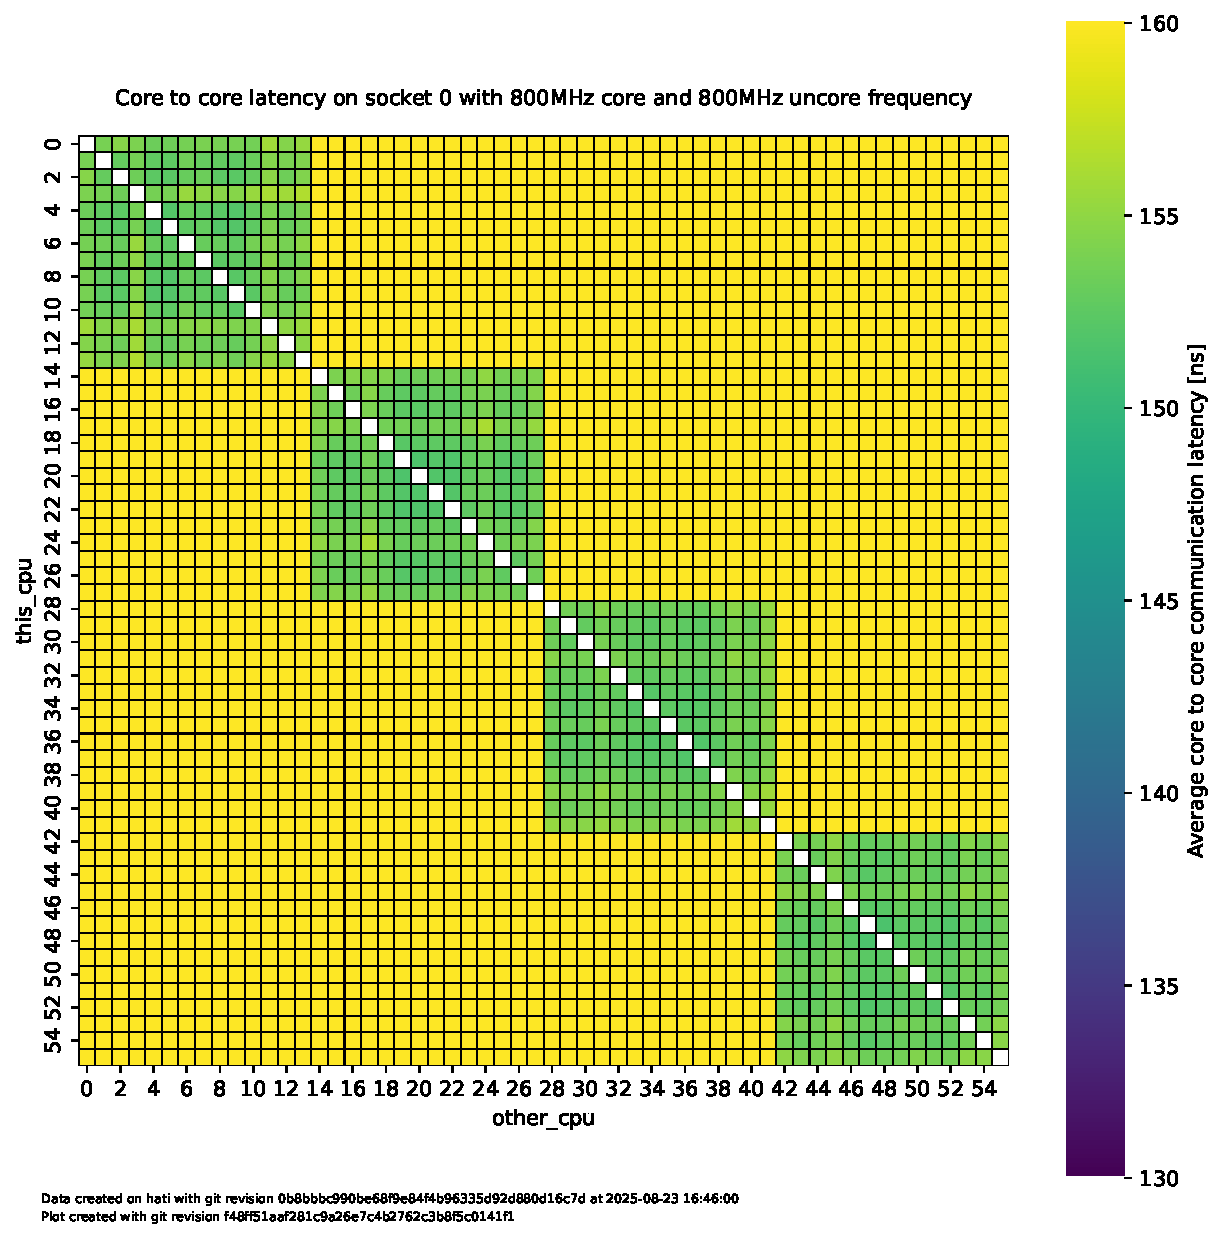
\includegraphics[width=\columnwidth]{fig/core-to-core-latency/core-to-core-heatmap-avg-800-800.pdf}
    \caption{Average core to core communication latency for hati's socket 0 with \SI{0.8}{\GHz} core and \SI{0.8}{\GHz} uncore frequency.}
\end{figure}
\begin{figure}[]
    \centering
    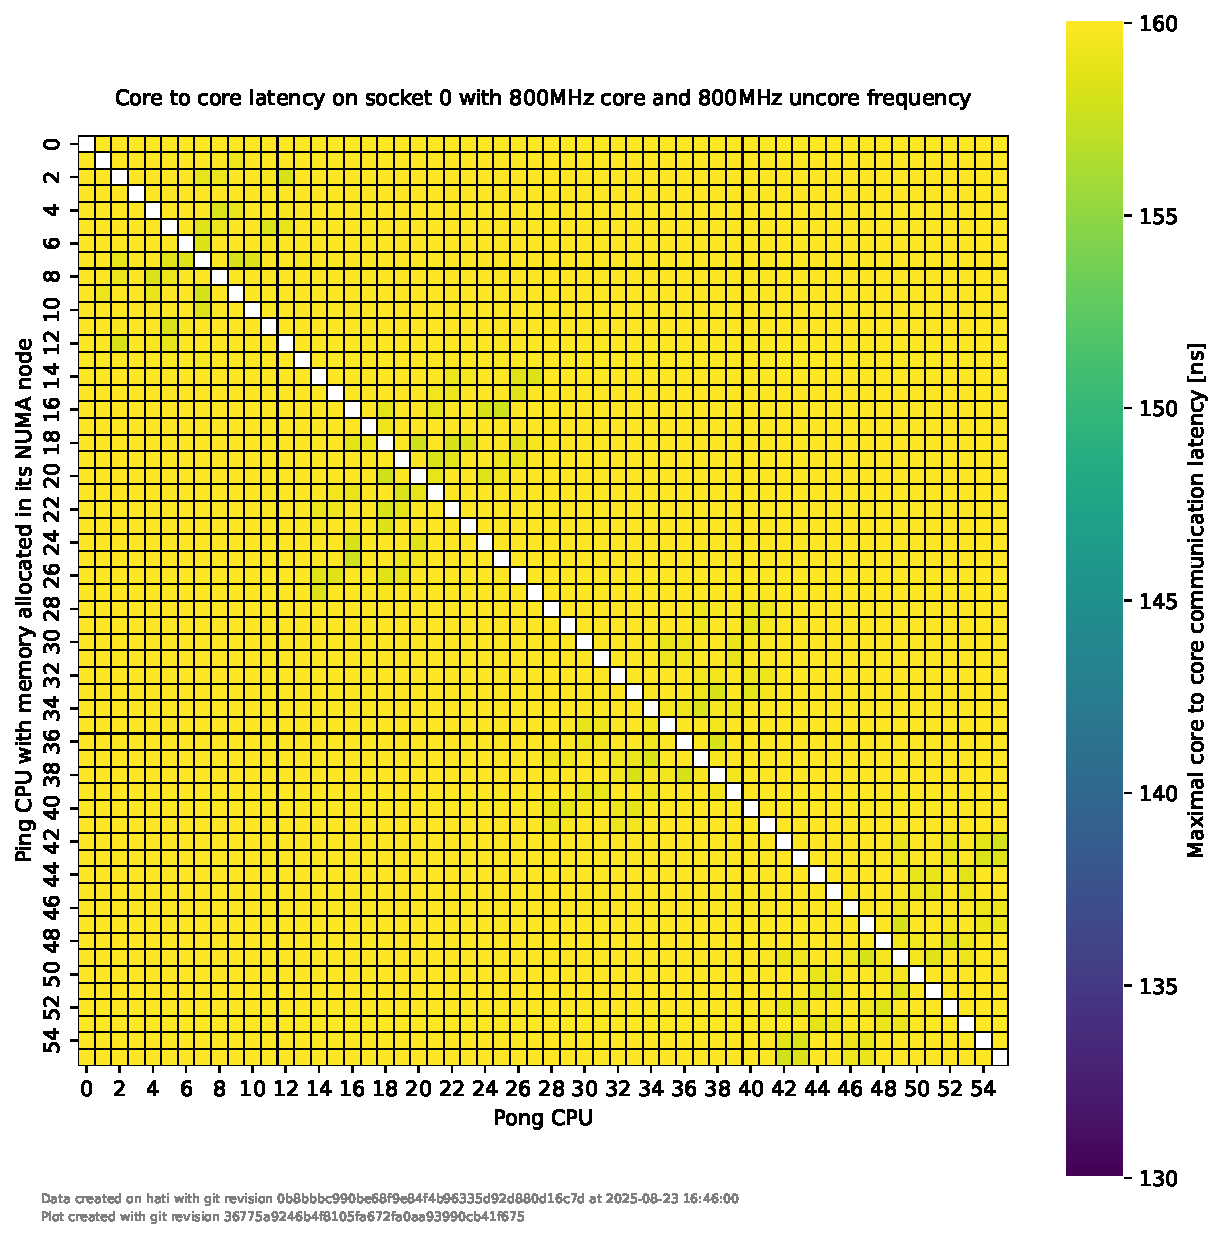
\includegraphics[width=\columnwidth]{fig/core-to-core-latency/core-to-core-heatmap-max-800-800.pdf}
    \caption{Maximimal core to core communication latency for hati's socket 0 with \SI{0.8}{\GHz} core and \SI{0.8}{\GHz} uncore frequency.}
\end{figure}
\begin{figure}[]
    \centering
    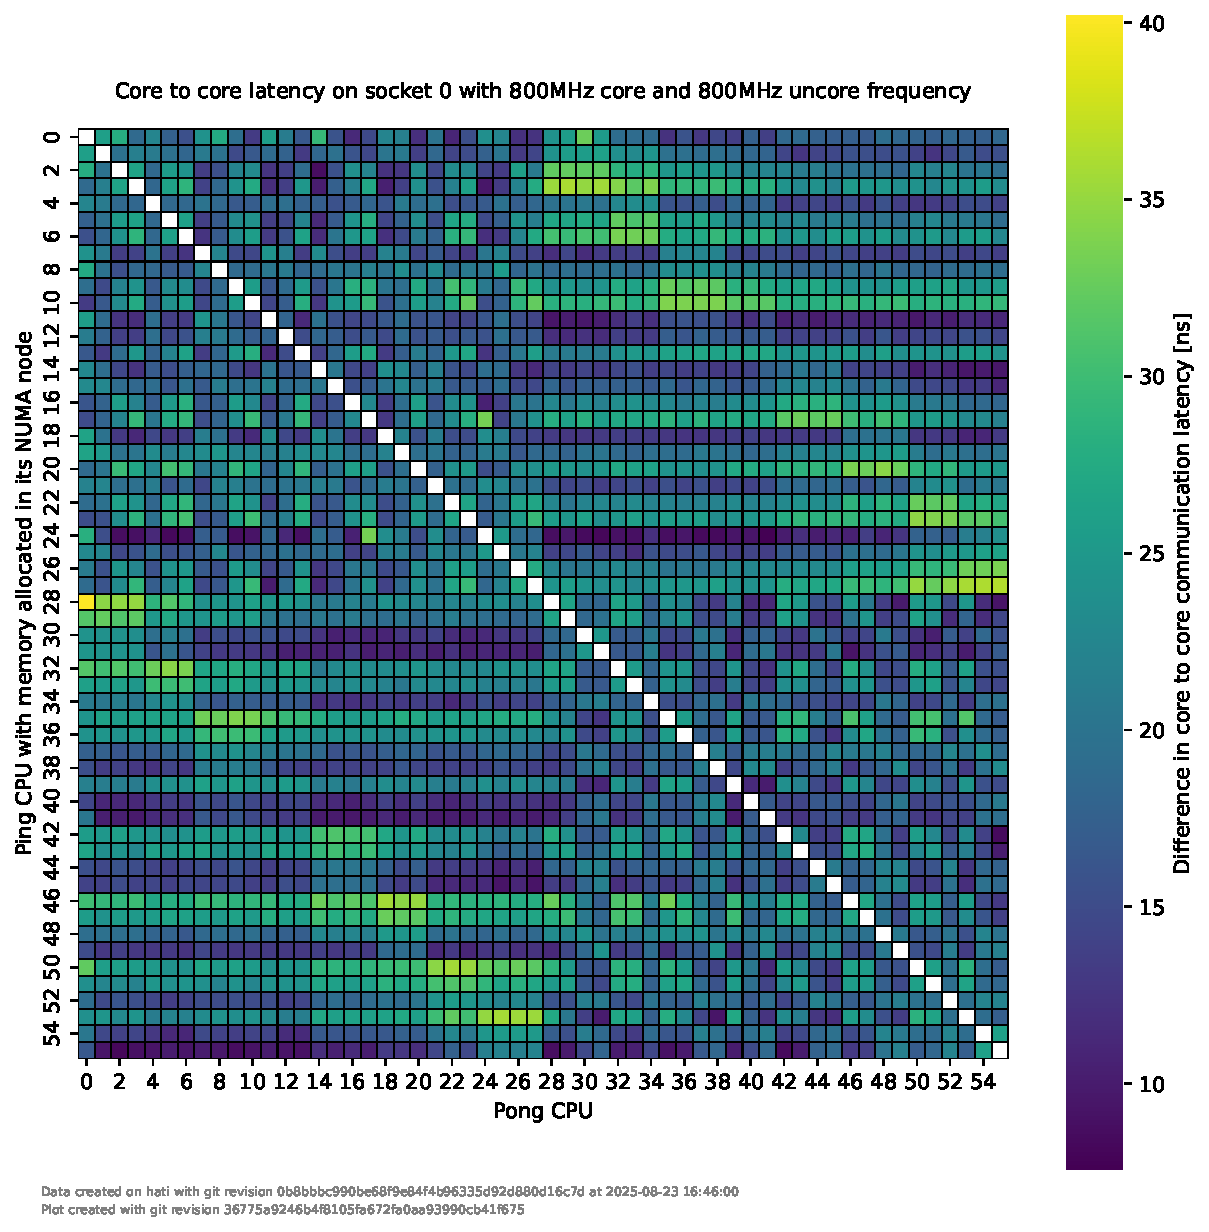
\includegraphics[width=\columnwidth]{fig/core-to-core-latency/core-to-core-heatmap-diff-800-800.pdf}
    \caption{Difference in core to core communication latency for hati's socket 0 with \SI{0.8}{\GHz} core and \SI{0.8}{\GHz} uncore frequency.}
\end{figure}

\begin{figure}[]
    \centering
    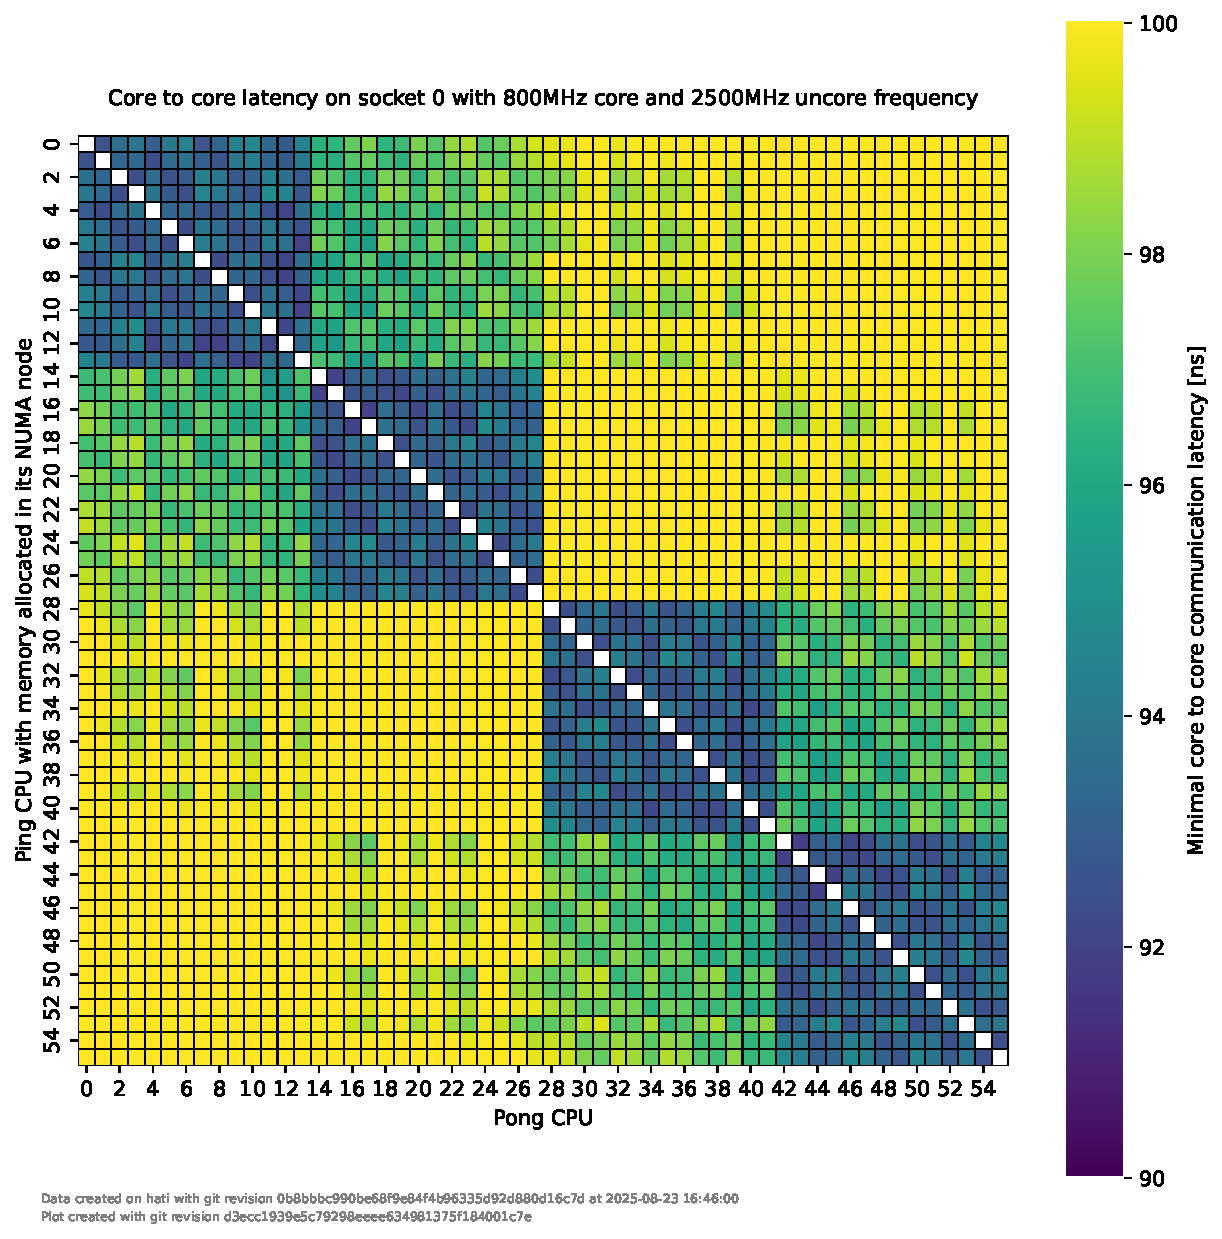
\includegraphics[width=\columnwidth]{fig/core-to-core-latency/core-to-core-heatmap-min-800-2500.pdf}
    \caption{Minimal core to core communication latency for hati's socket 0 with \SI{0.8}{\GHz} core and \SI{2.5}{\GHz} uncore frequency.}
\end{figure}
\begin{figure}[]
    \centering
    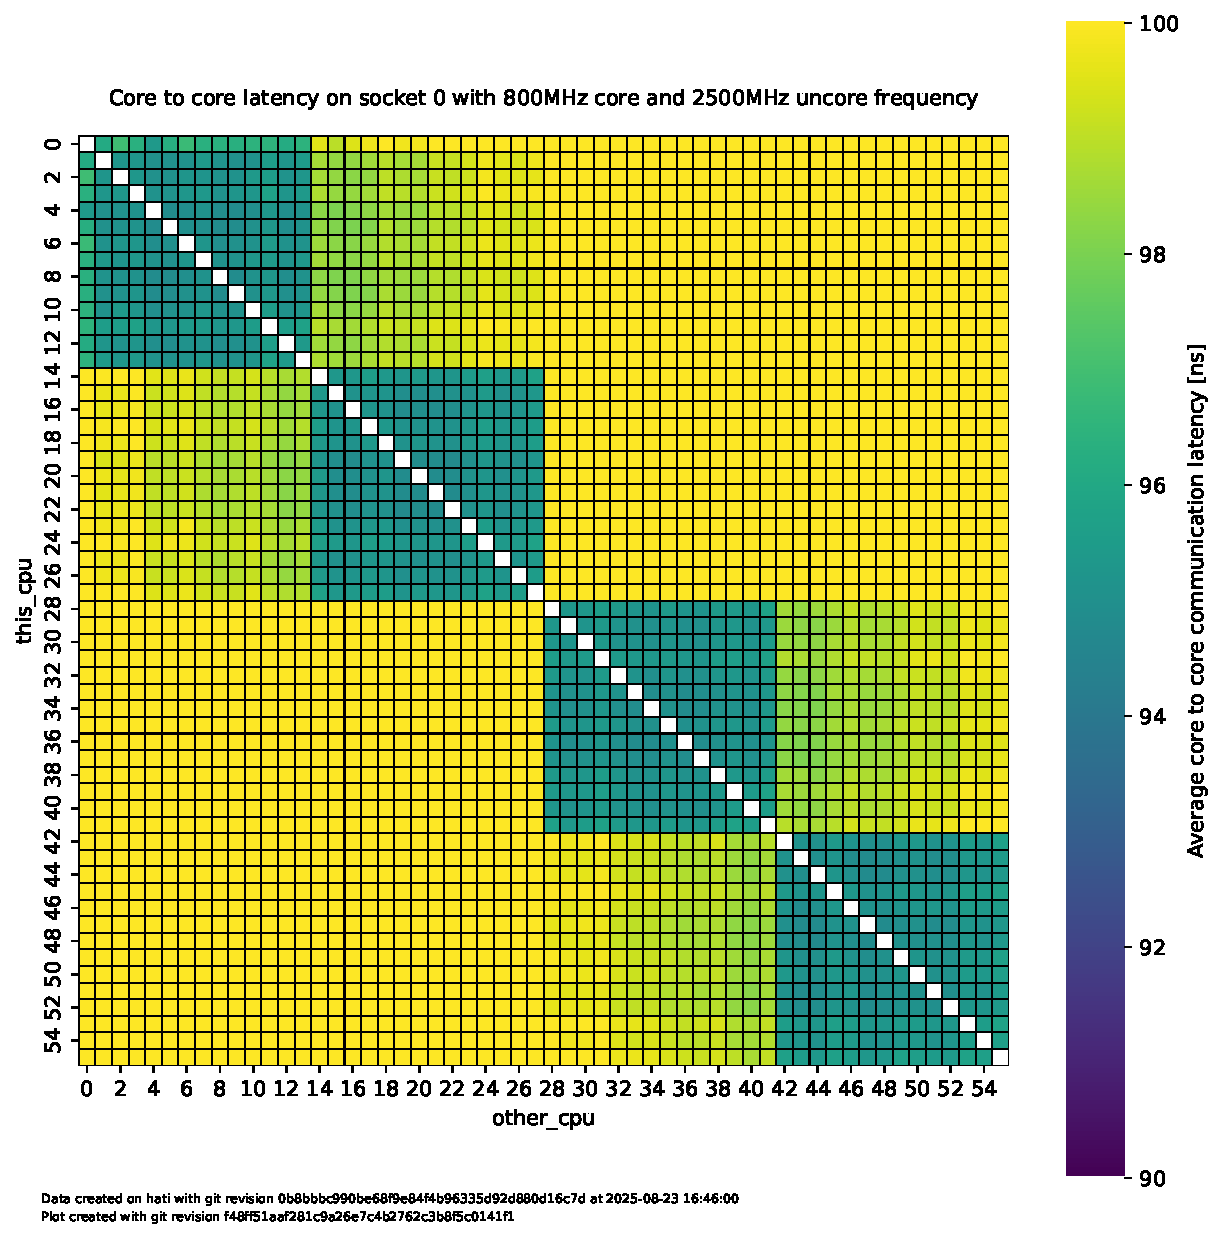
\includegraphics[width=\columnwidth]{fig/core-to-core-latency/core-to-core-heatmap-avg-800-2500.pdf}
    \caption{Average core to core communication latency for hati's socket 0 with \SI{0.8}{\GHz} core and \SI{2.5}{\GHz} uncore frequency.}
\end{figure}
\begin{figure}[]
    \centering
    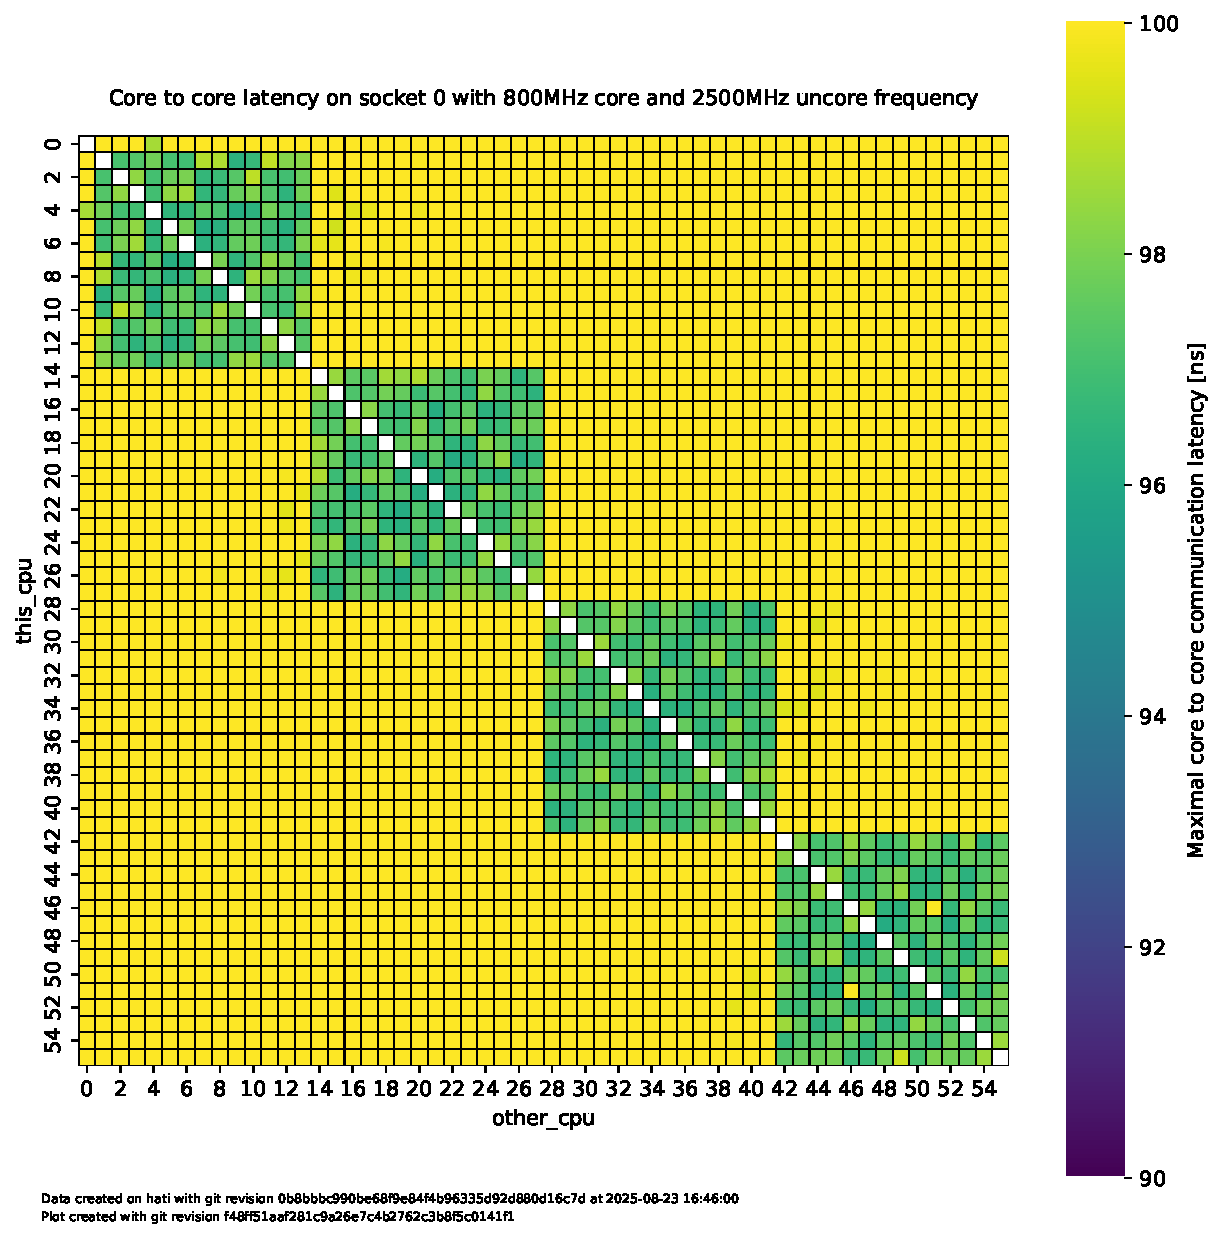
\includegraphics[width=\columnwidth]{fig/core-to-core-latency/core-to-core-heatmap-max-800-2500.pdf}
    \caption{Maximimal core to core communication latency for hati's socket 0 with \SI{0.8}{\GHz} core and \SI{2.5}{\GHz} uncore frequency.}
\end{figure}
\begin{figure}[]
    \centering
    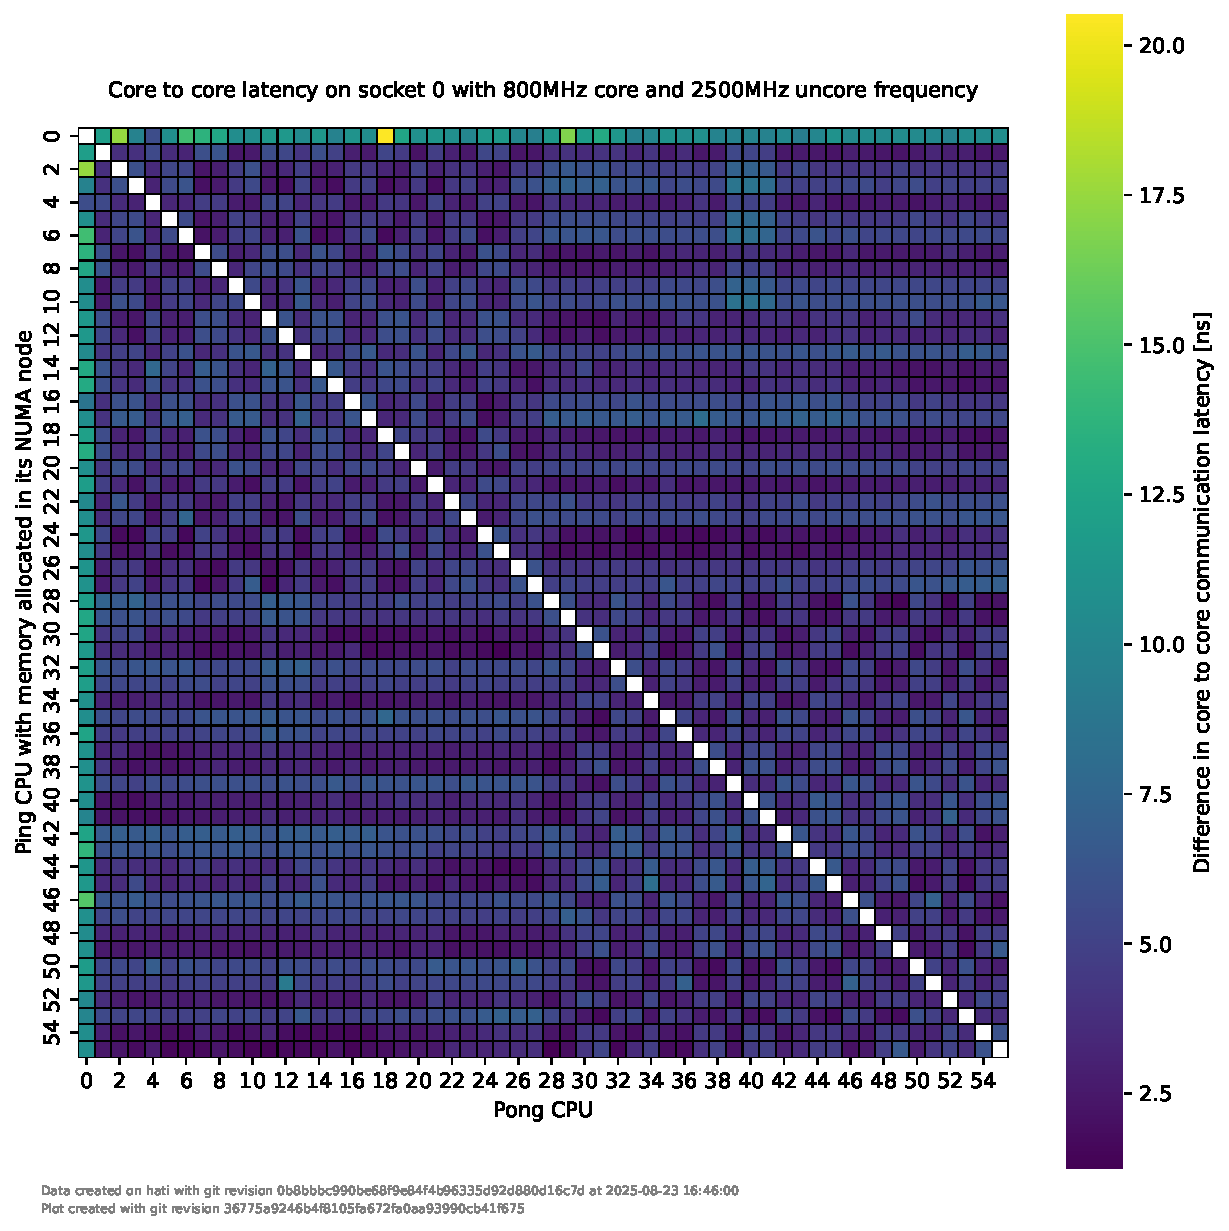
\includegraphics[width=\columnwidth]{fig/core-to-core-latency/core-to-core-heatmap-diff-800-2500.pdf}
    \caption{Difference in core to core communication latency for hati's socket 0 with \SI{0.8}{\GHz} core and \SI{2.5}{\GHz} uncore frequency.}
\end{figure}

\begin{figure}[]
    \centering
    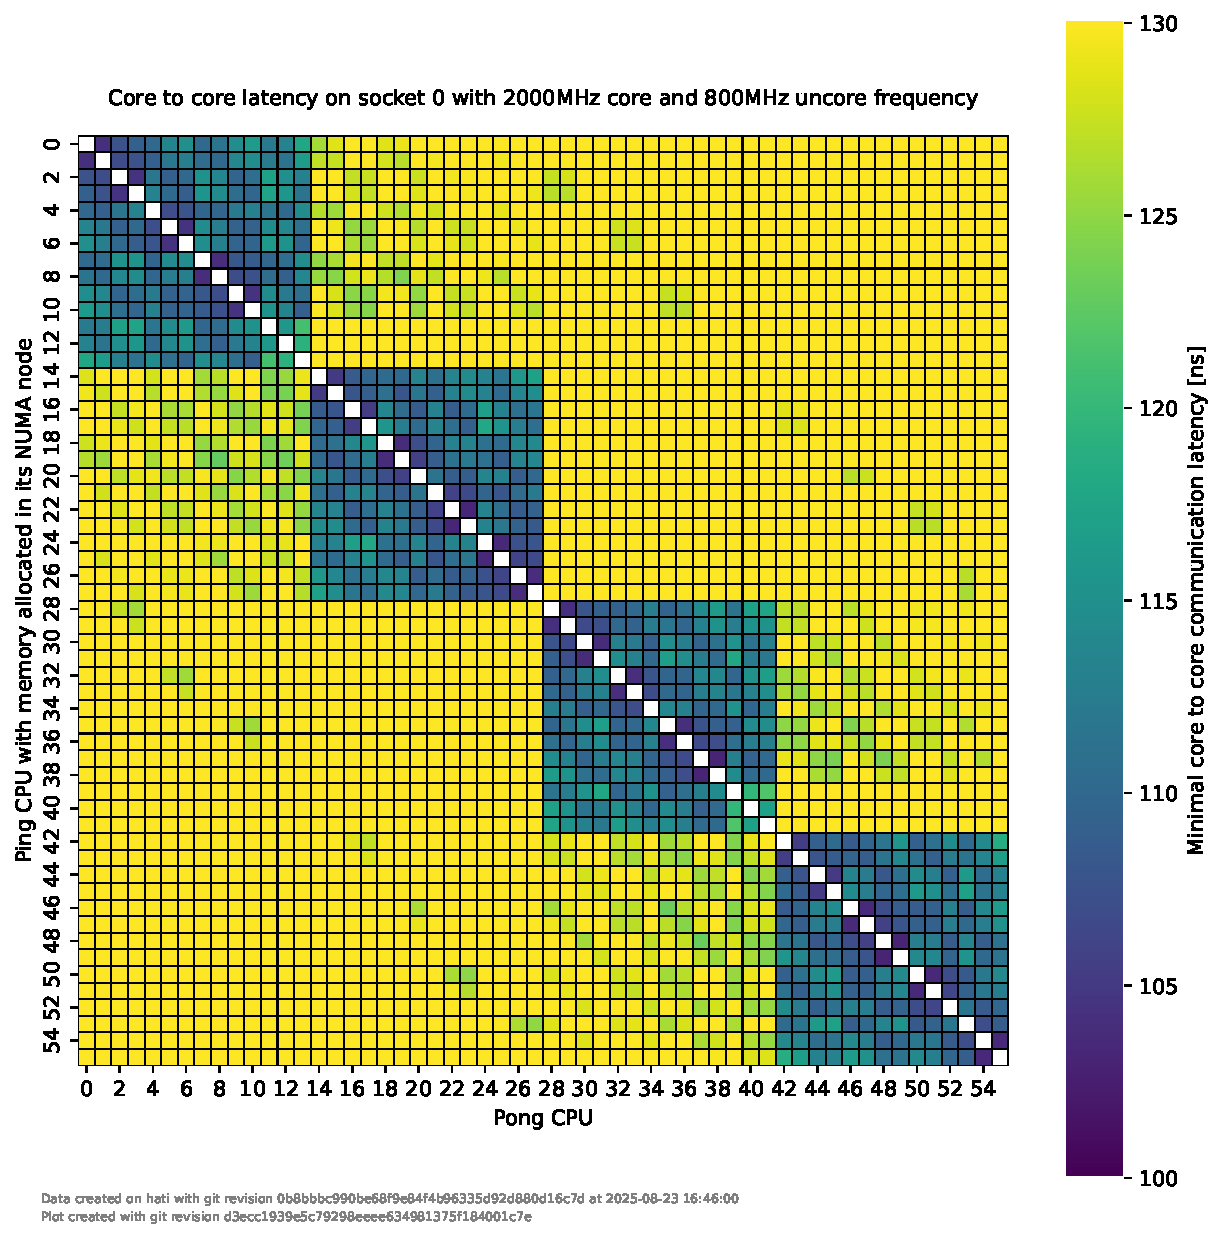
\includegraphics[width=\columnwidth]{fig/core-to-core-latency/core-to-core-heatmap-min-2000-800.pdf}
    \caption{Minimal core to core communication latency for hati's socket 0 with \SI{2.0}{\GHz} core and \SI{0.8}{\GHz} uncore frequency.}
\end{figure}
\begin{figure}[]
    \centering
    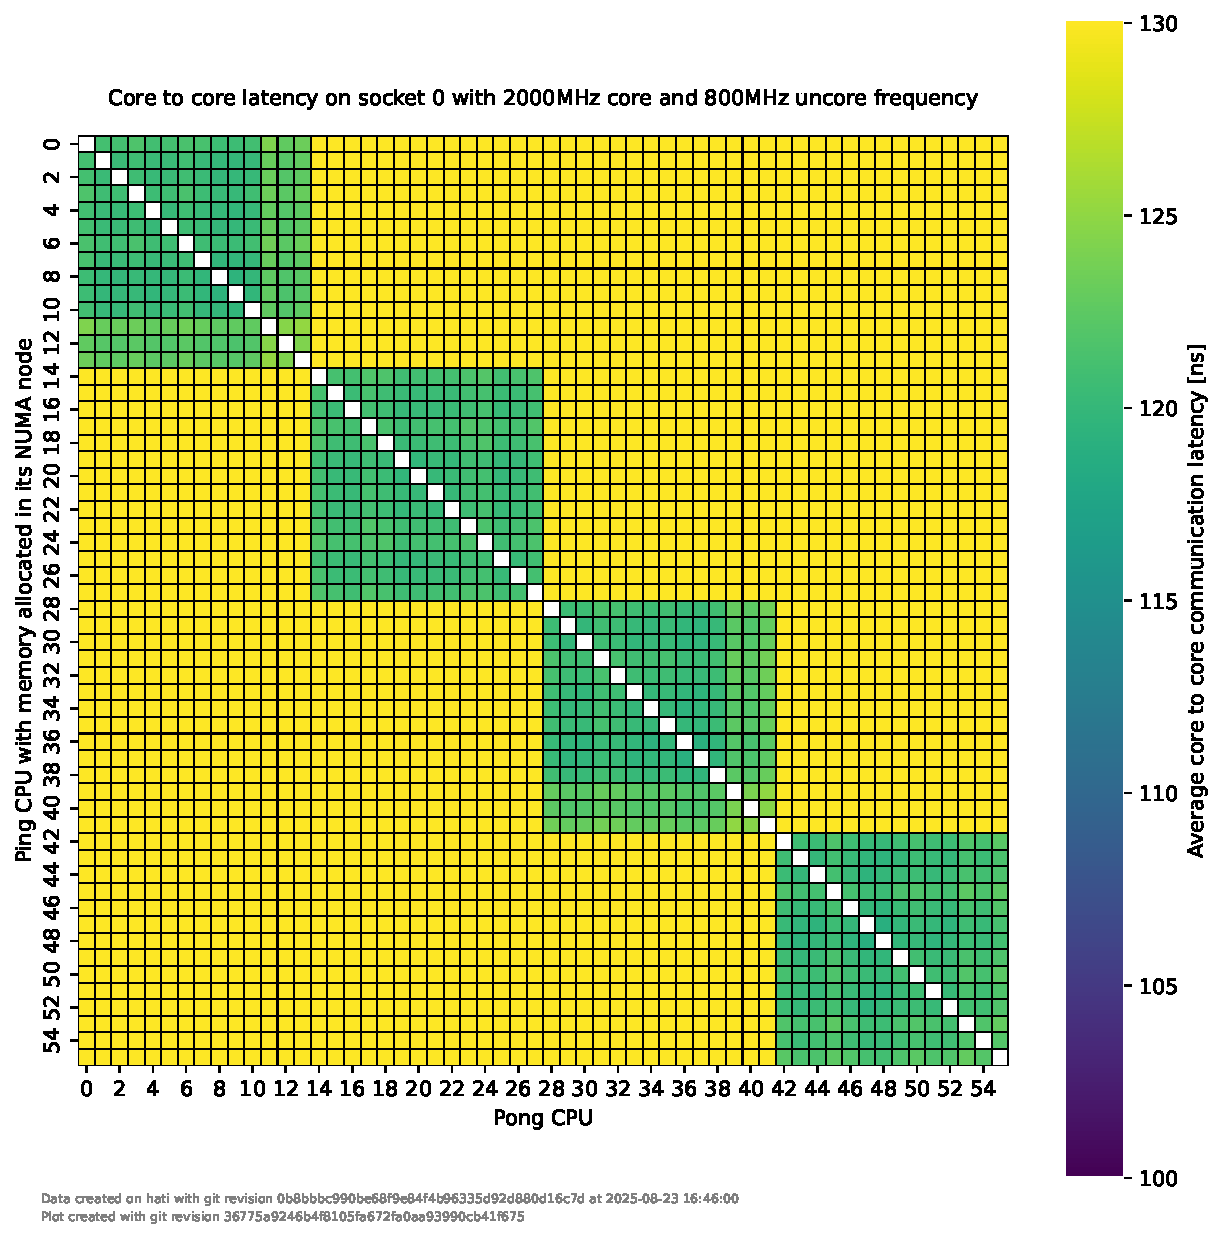
\includegraphics[width=\columnwidth]{fig/core-to-core-latency/core-to-core-heatmap-avg-2000-800.pdf}
    \caption{Average core to core communication latency for hati's socket 0 with \SI{2.0}{\GHz} core and \SI{0.8}{\GHz} uncore frequency.}
\end{figure}
\begin{figure}[]
    \centering
    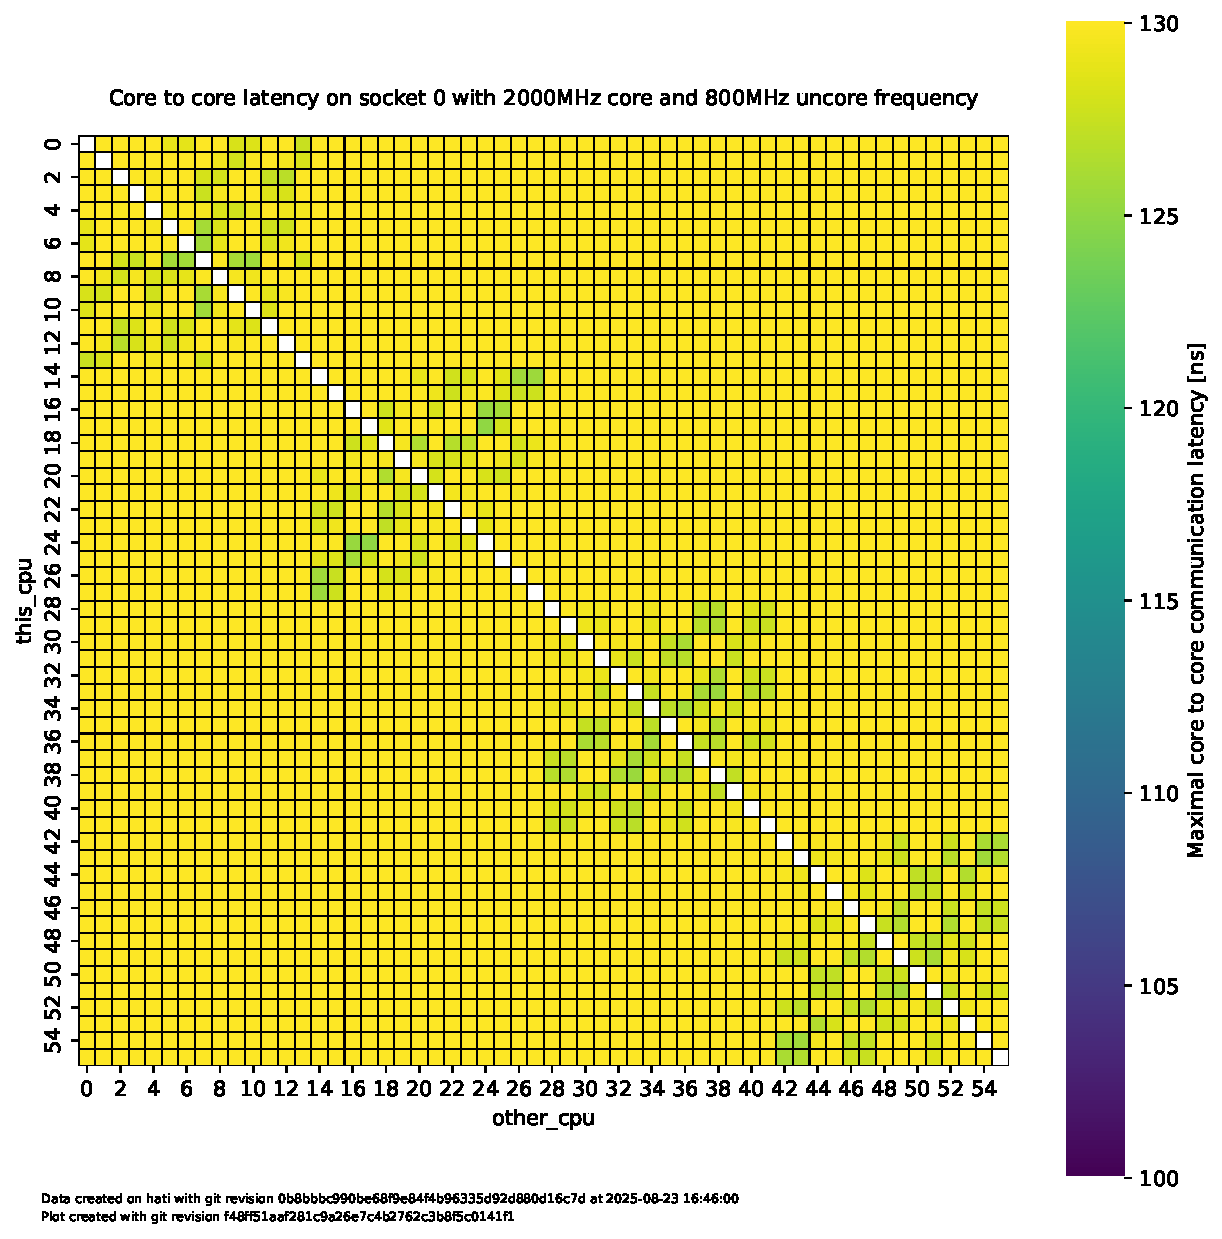
\includegraphics[width=\columnwidth]{fig/core-to-core-latency/core-to-core-heatmap-max-2000-800.pdf}
    \caption{Maximimal core to core communication latency for hati's socket 0 with \SI{2.0}{\GHz} core and \SI{0.8}{\GHz} uncore frequency.}
\end{figure}
\begin{figure}[]
    \centering
    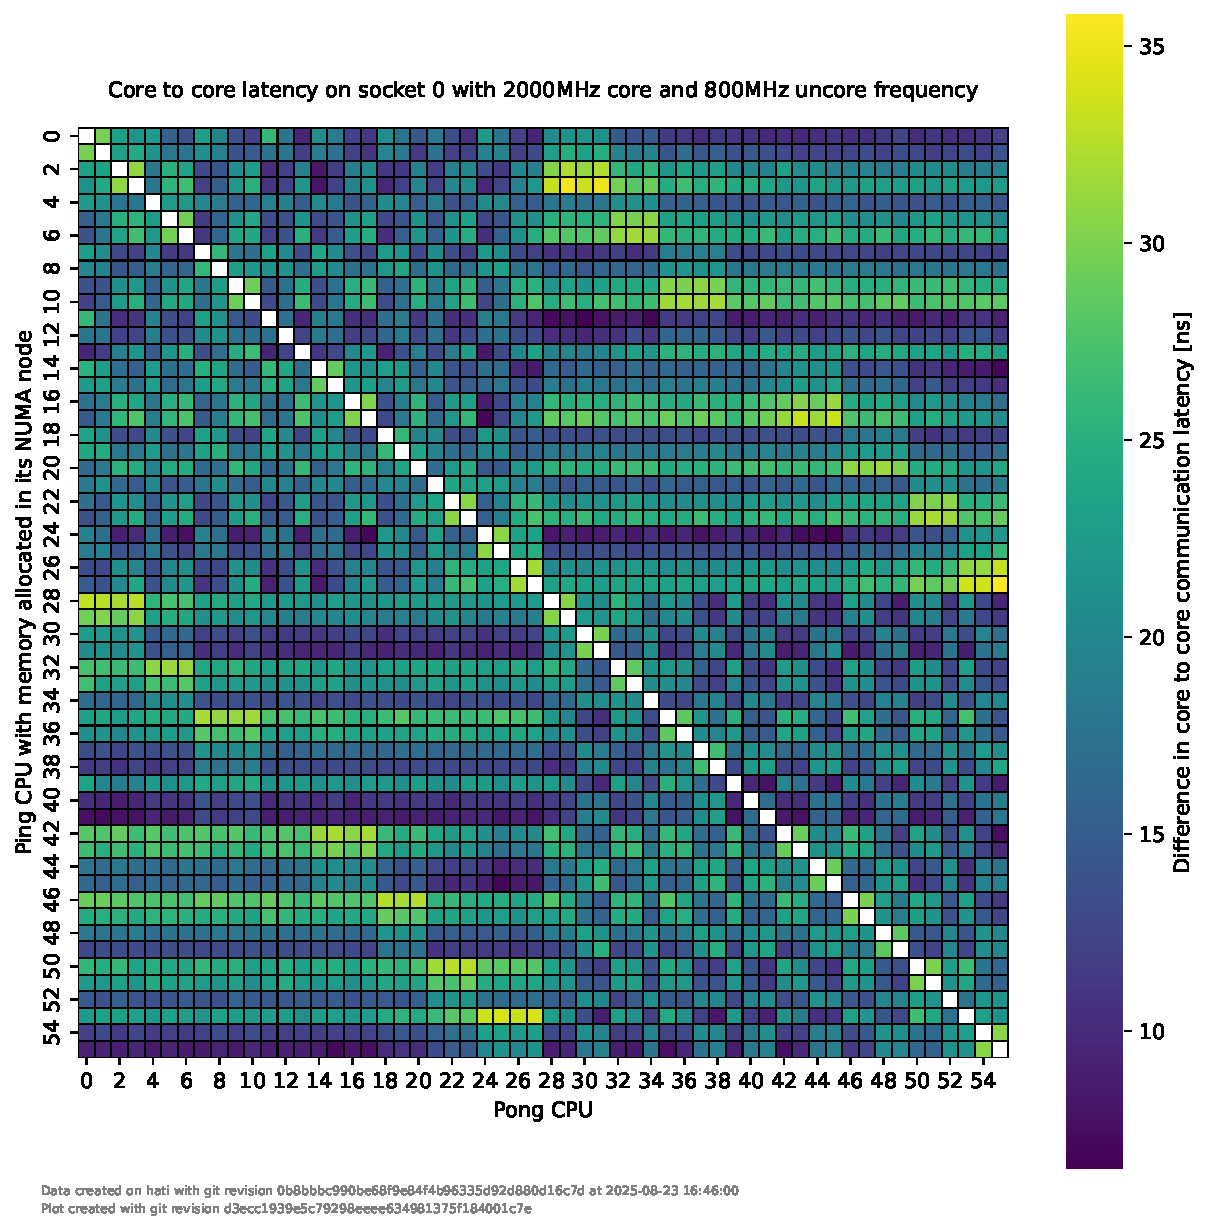
\includegraphics[width=\columnwidth]{fig/core-to-core-latency/core-to-core-heatmap-diff-2000-800.pdf}
    \caption{Difference in core to core communication latency for hati's socket 0 with \SI{2.0}{\GHz} core and \SI{0.8}{\GHz} uncore frequency.}
\end{figure}

\begin{figure}[]
    \centering
    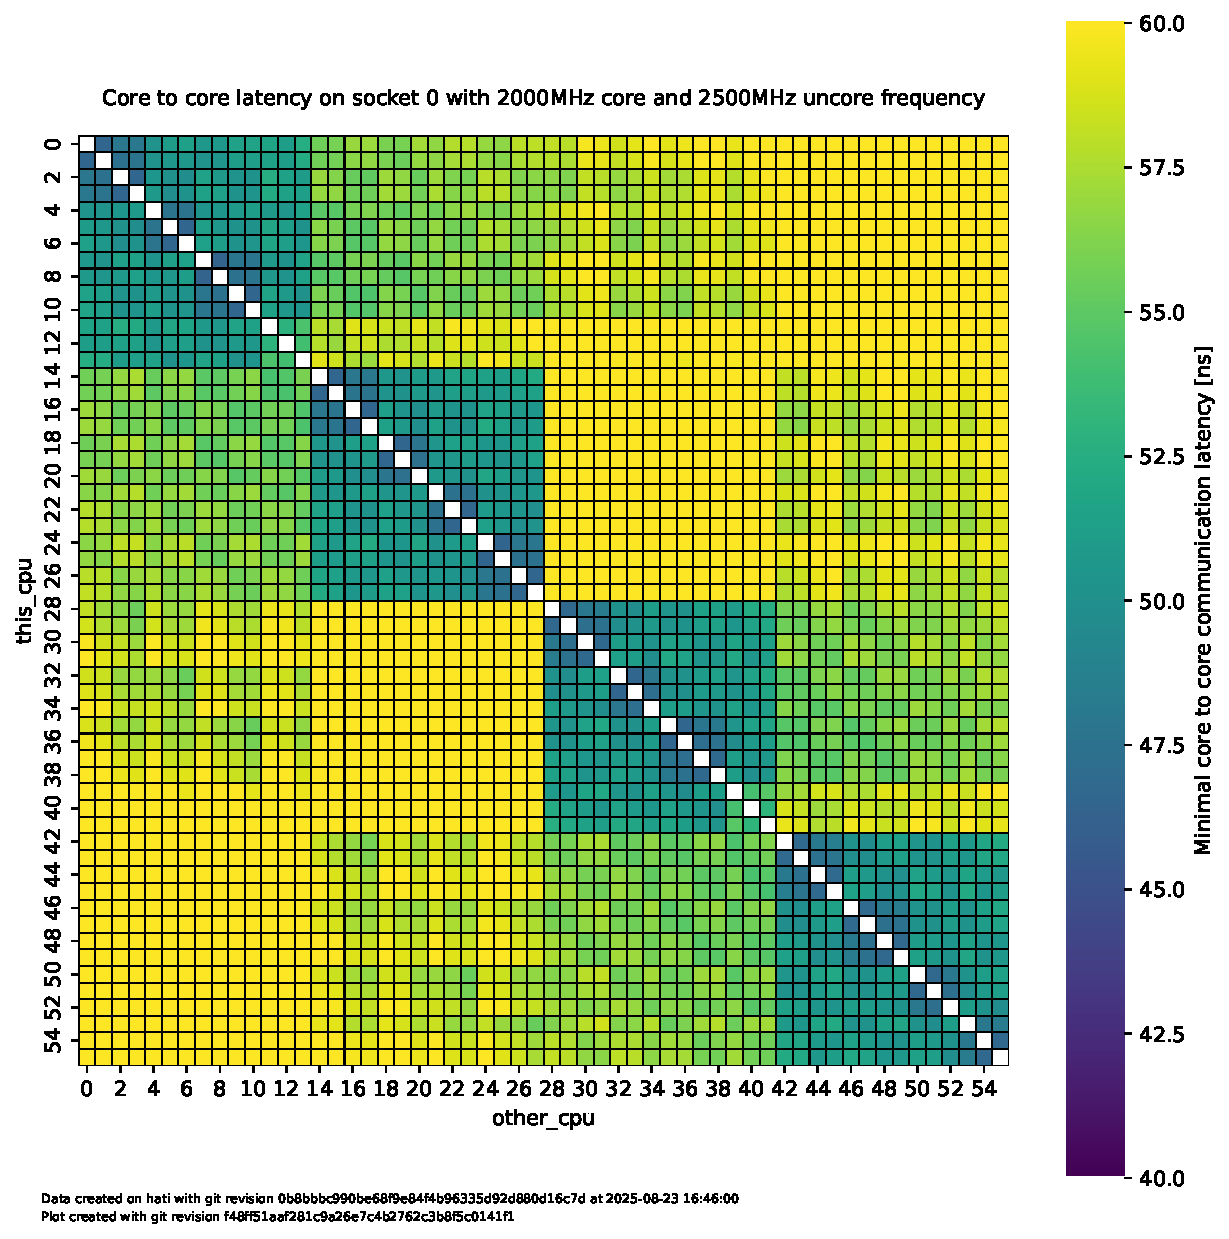
\includegraphics[width=\columnwidth]{fig/core-to-core-latency/core-to-core-heatmap-min-2000-2500.pdf}
    \caption{Minimal core to core communication latency for hati's socket 0 with \SI{2.0}{\GHz} core and \SI{2.5}{\GHz} uncore frequency.}
\end{figure}
\begin{figure}[]
    \centering
    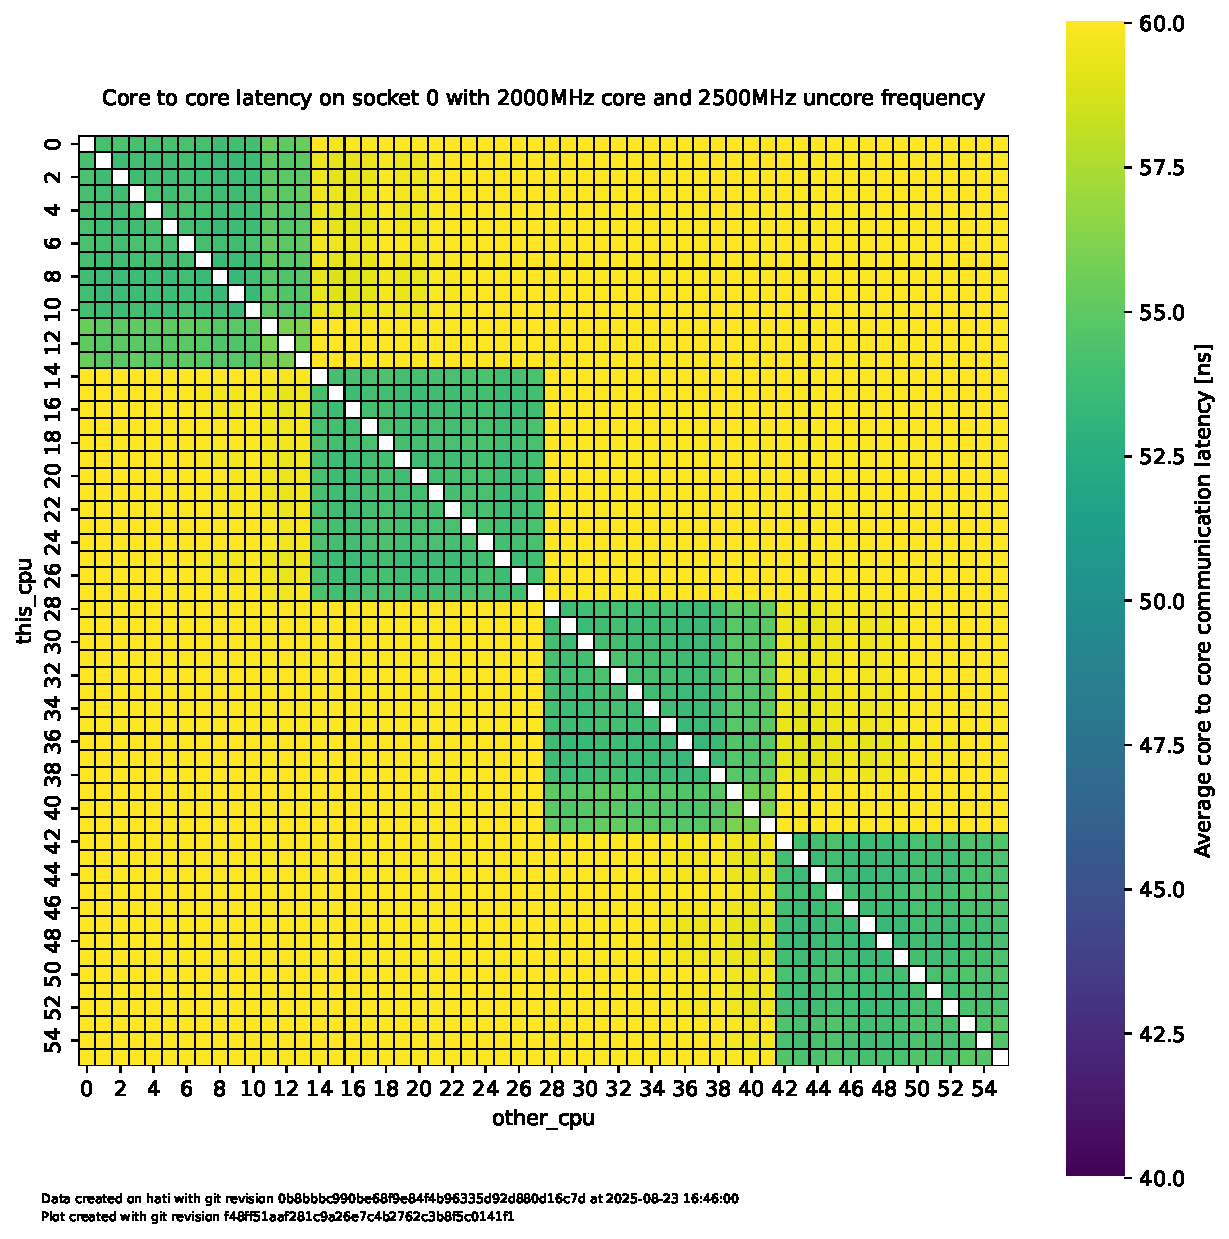
\includegraphics[width=\columnwidth]{fig/core-to-core-latency/core-to-core-heatmap-avg-2000-2500.pdf}
    \caption{Average core to core communication latency for hati's socket 0 with \SI{2.0}{\GHz} core and \SI{2.5}{\GHz} uncore frequency.}
\end{figure}
\begin{figure}[]
    \centering
    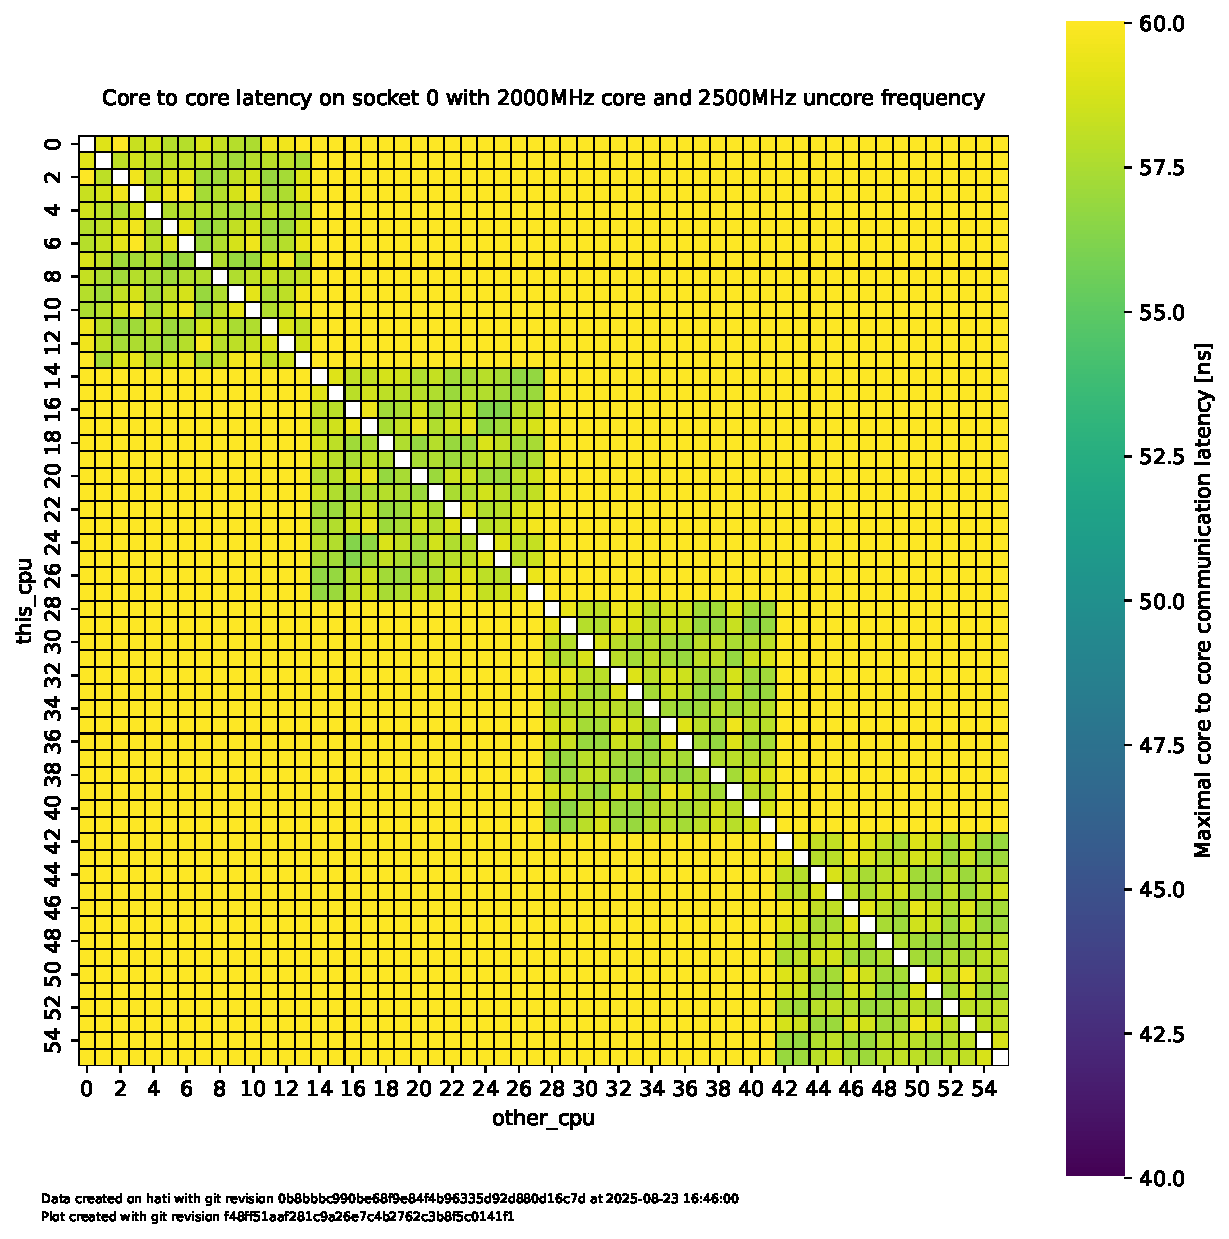
\includegraphics[width=\columnwidth]{fig/core-to-core-latency/core-to-core-heatmap-max-2000-2500.pdf}
    \caption{Maximimal core to core communication latency for hati's socket 0 with \SI{2.0}{\GHz} core and \SI{2.5}{\GHz} uncore frequency.}
\end{figure}
\begin{figure}[]
    \centering
    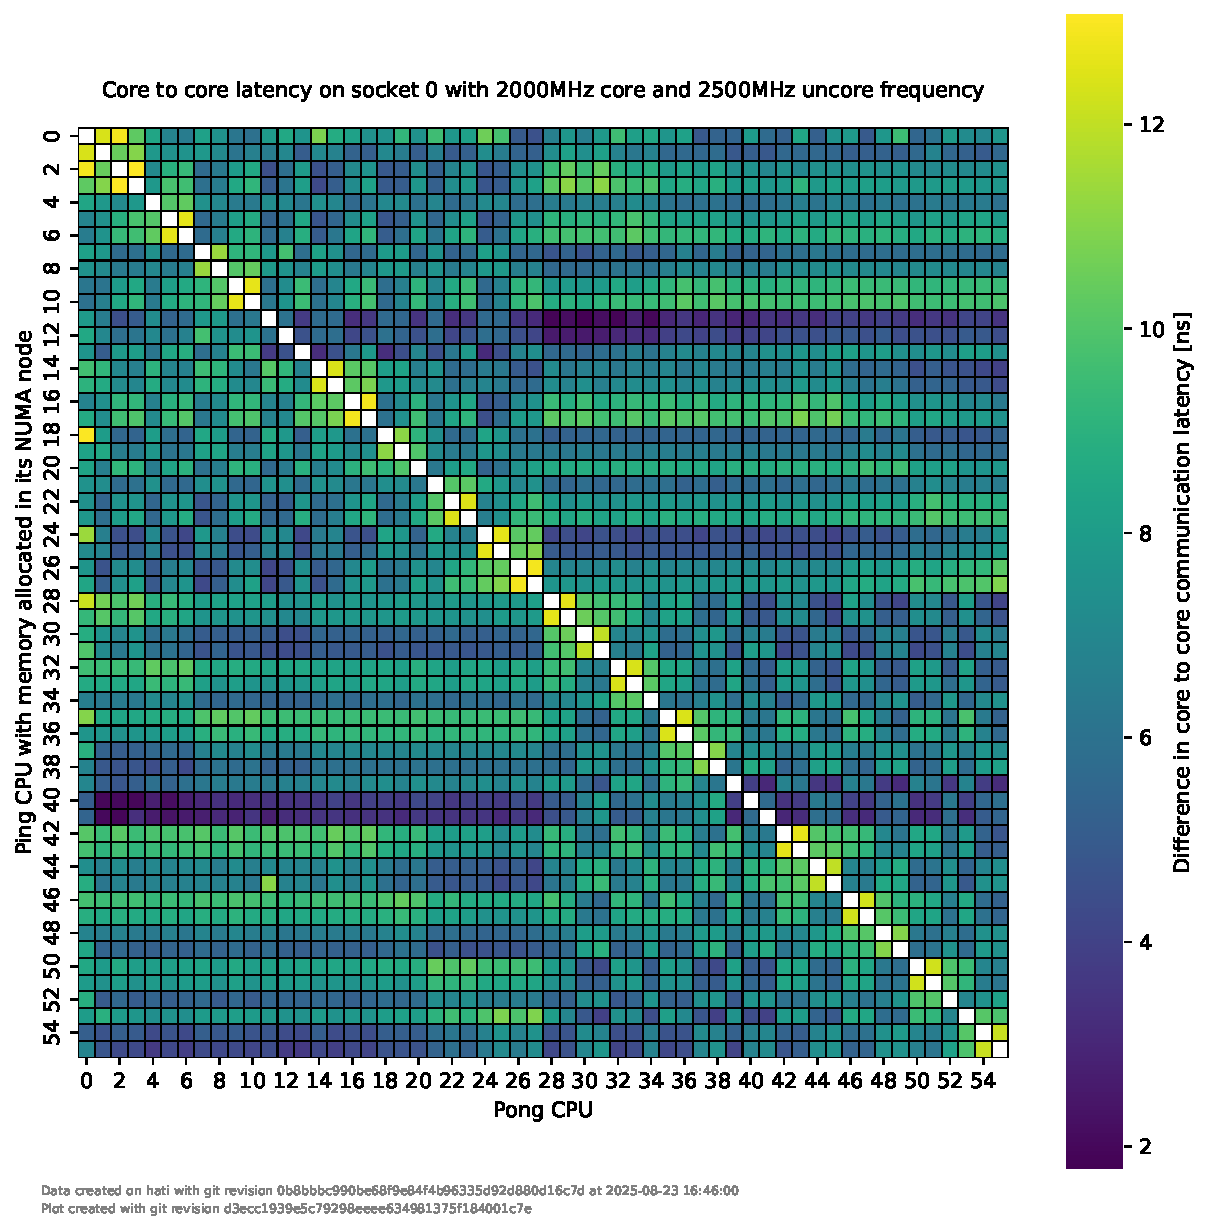
\includegraphics[width=\columnwidth]{fig/core-to-core-latency/core-to-core-heatmap-diff-2000-2500.pdf}
    \caption{Difference in core to core communication latency for hati's socket 0 with \SI{2.0}{\GHz} core and \SI{2.5}{\GHz} uncore frequency.}
\end{figure}

\begin{figure}[]
    \centering
    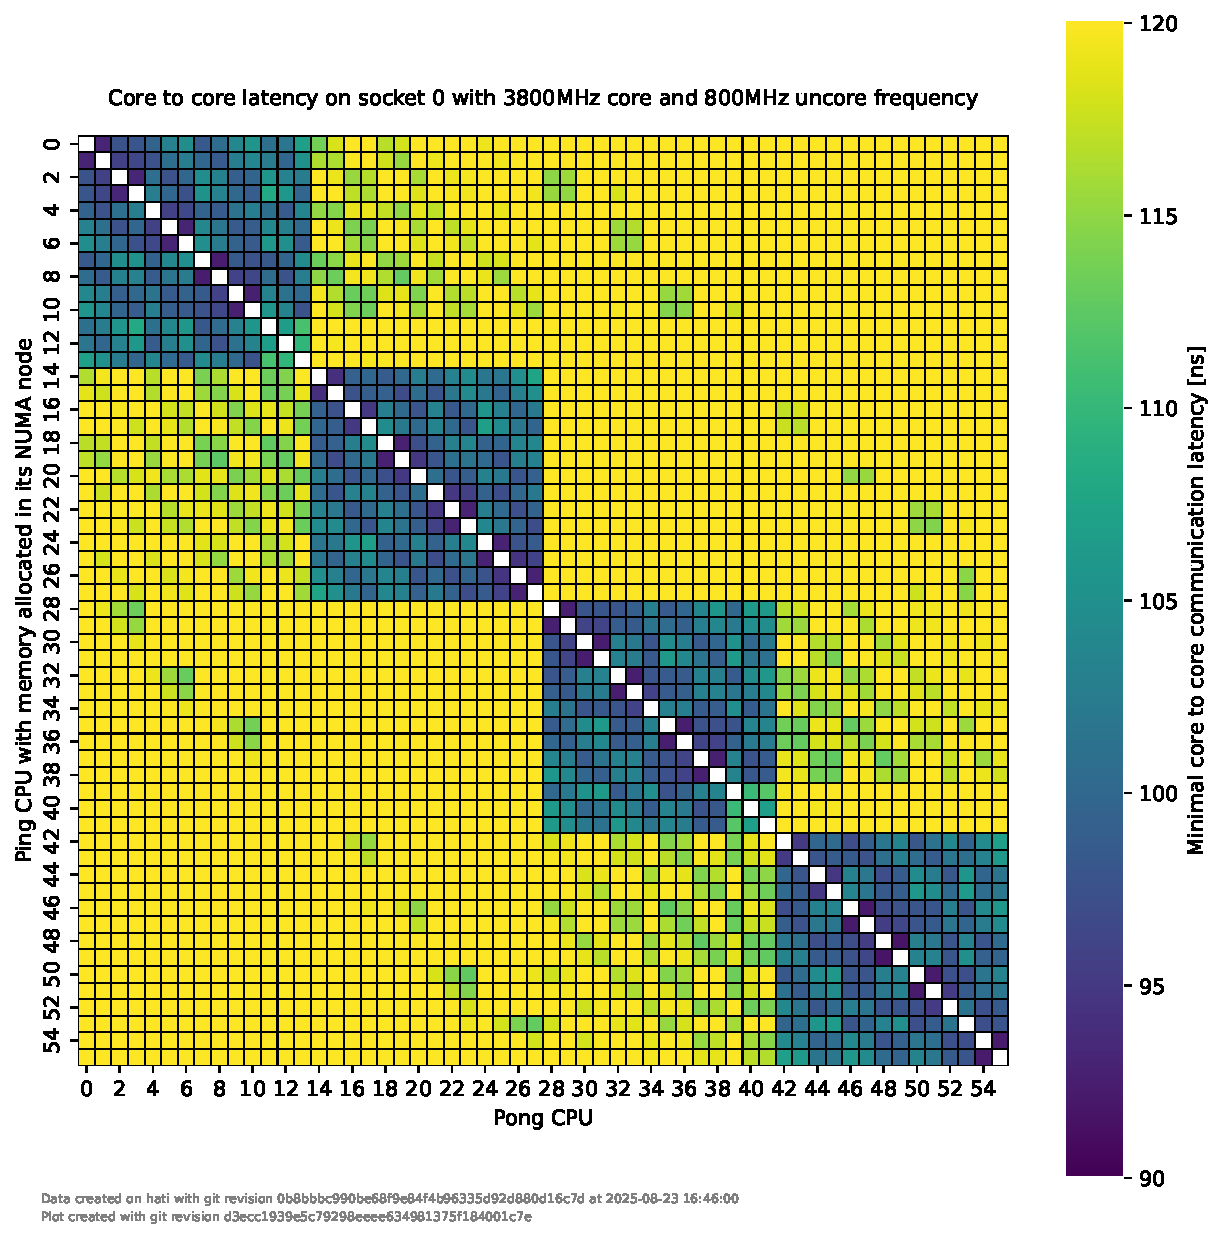
\includegraphics[width=\columnwidth]{fig/core-to-core-latency/core-to-core-heatmap-min-3800-800.pdf}
    \caption{Minimal core to core communication latency for hati's socket 0 with \SI{3.8}{\GHz} core and \SI{0.8}{\GHz} uncore frequency.}
\end{figure}
\begin{figure}[]
    \centering
    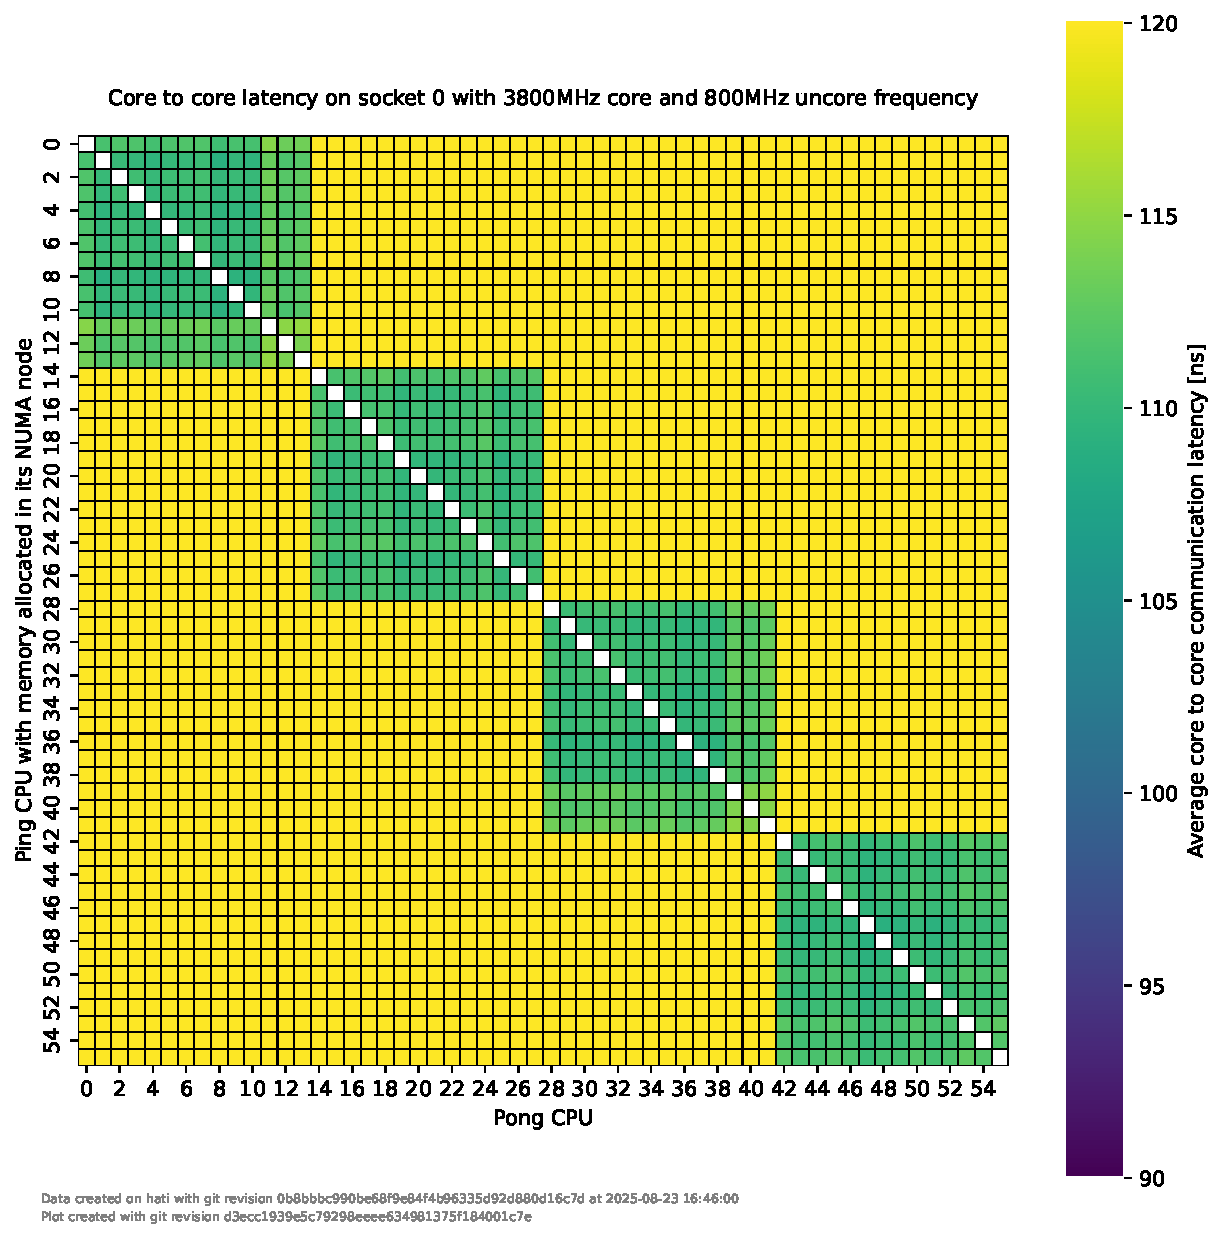
\includegraphics[width=\columnwidth]{fig/core-to-core-latency/core-to-core-heatmap-avg-3800-800.pdf}
    \caption{Average core to core communication latency for hati's socket 0 with \SI{3.8}{\GHz} core and \SI{0.8}{\GHz} uncore frequency.}
\end{figure}
\begin{figure}[]
    \centering
    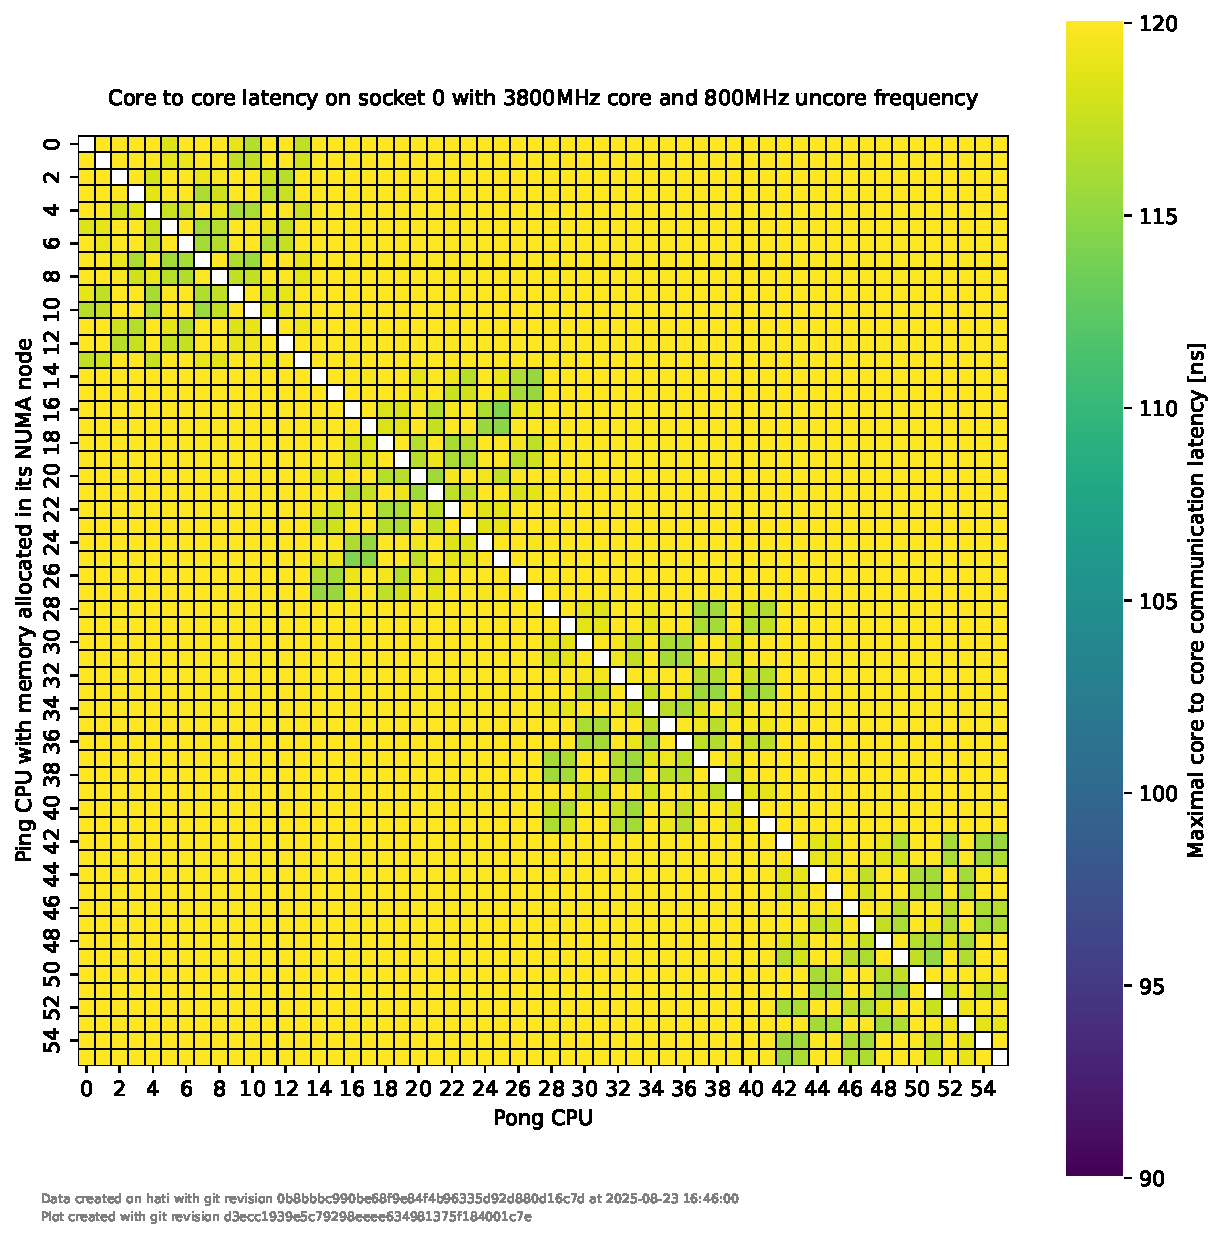
\includegraphics[width=\columnwidth]{fig/core-to-core-latency/core-to-core-heatmap-max-3800-800.pdf}
    \caption{Maximimal core to core communication latency for hati's socket 0 with \SI{3.8}{\GHz} core and \SI{0.8}{\GHz} uncore frequency.}
\end{figure}
\begin{figure}[]
    \centering
    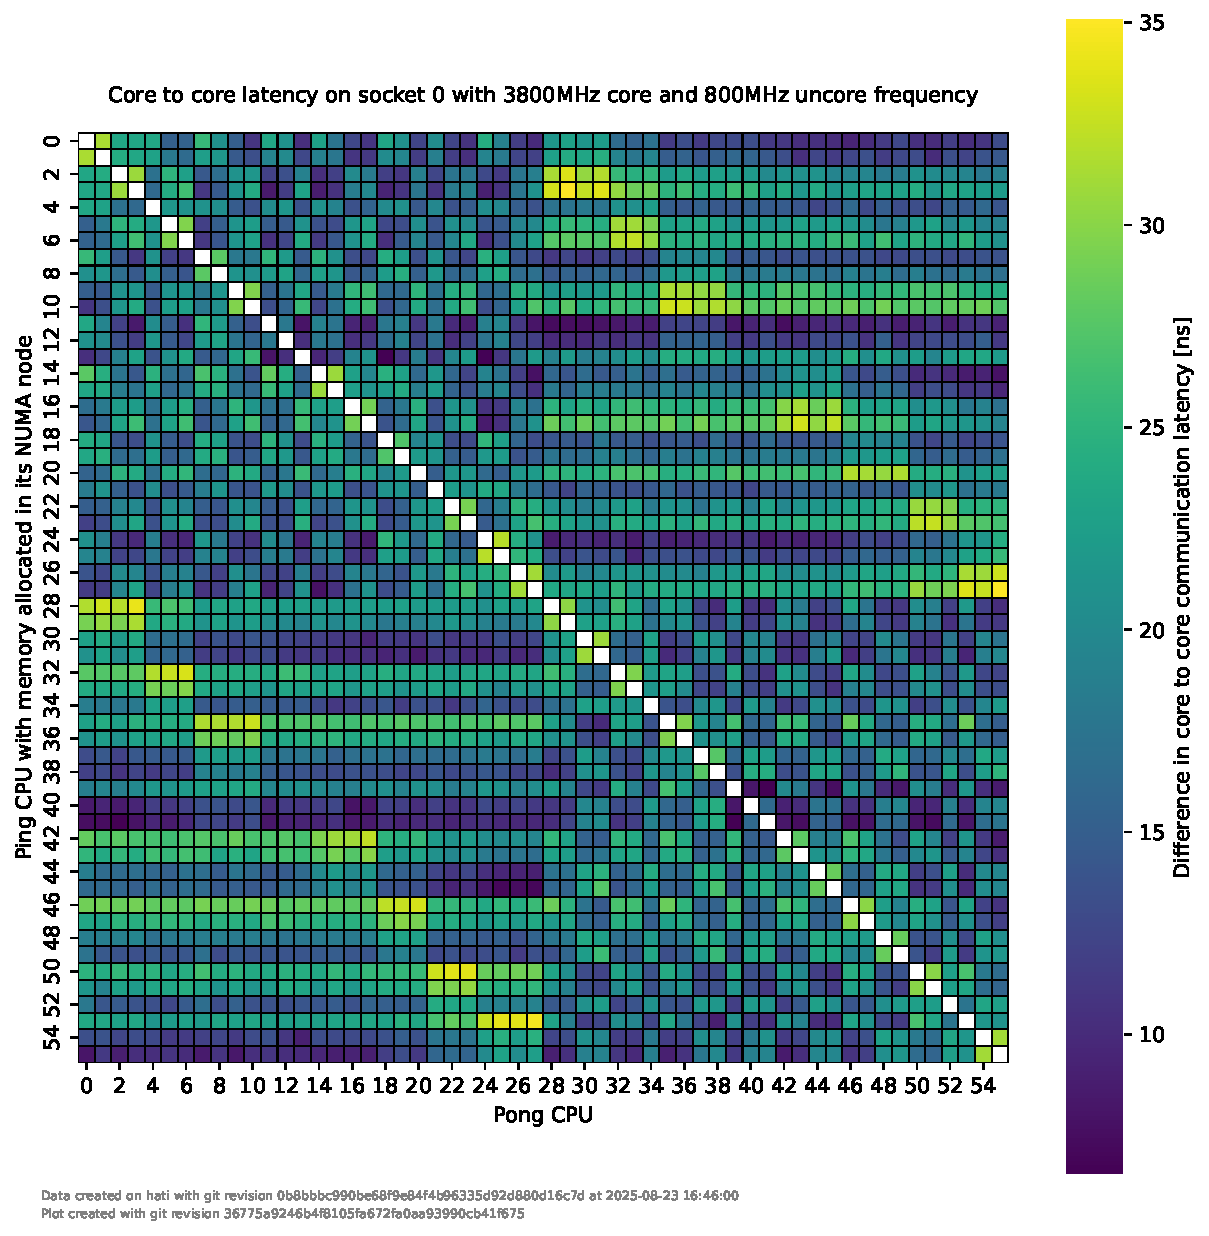
\includegraphics[width=\columnwidth]{fig/core-to-core-latency/core-to-core-heatmap-diff-3800-800.pdf}
    \caption{Difference in core to core communication latency for hati's socket 0 with \SI{3.8}{\GHz} core and \SI{0.8}{\GHz} uncore frequency.}
\end{figure}

\begin{figure}[]
    \centering
    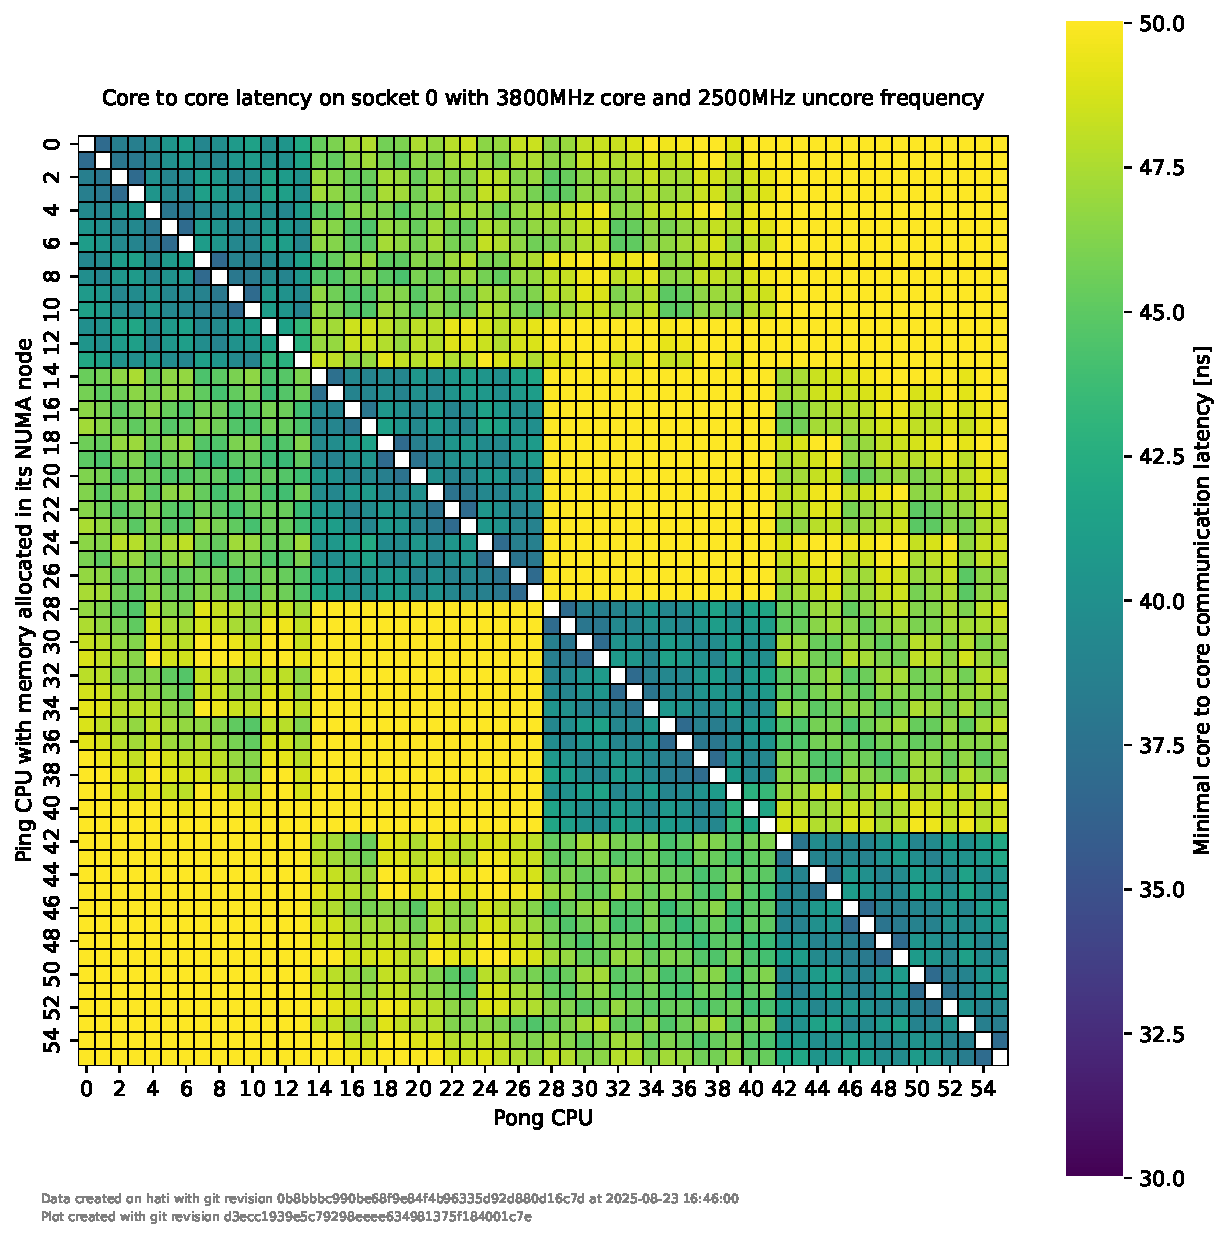
\includegraphics[width=\columnwidth]{fig/core-to-core-latency/core-to-core-heatmap-min-3800-2500.pdf}
    \caption{Minimal core to core communication latency for hati's socket 0 with \SI{3.8}{\GHz} core and \SI{2.5}{\GHz} uncore frequency.}
\end{figure}
\begin{figure}[]
    \centering
    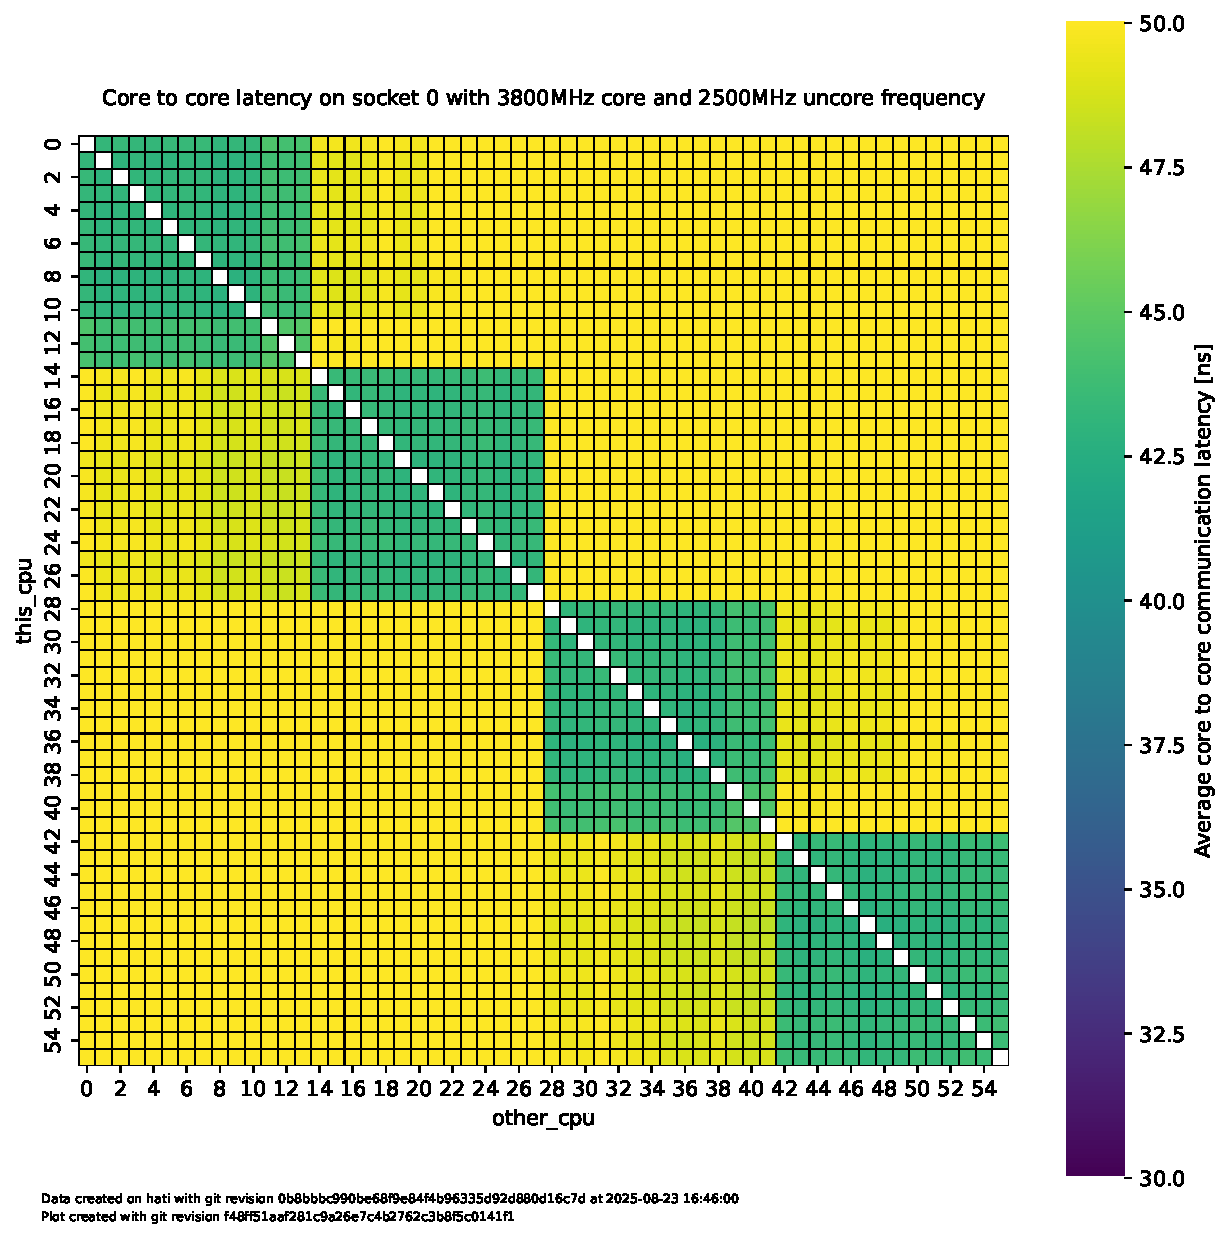
\includegraphics[width=\columnwidth]{fig/core-to-core-latency/core-to-core-heatmap-avg-3800-2500.pdf}
    \caption{Average core to core communication latency for hati's socket 0 with \SI{3.8}{\GHz} core and \SI{2.5}{\GHz} uncore frequency.}
\end{figure}
\begin{figure}[]
    \centering
    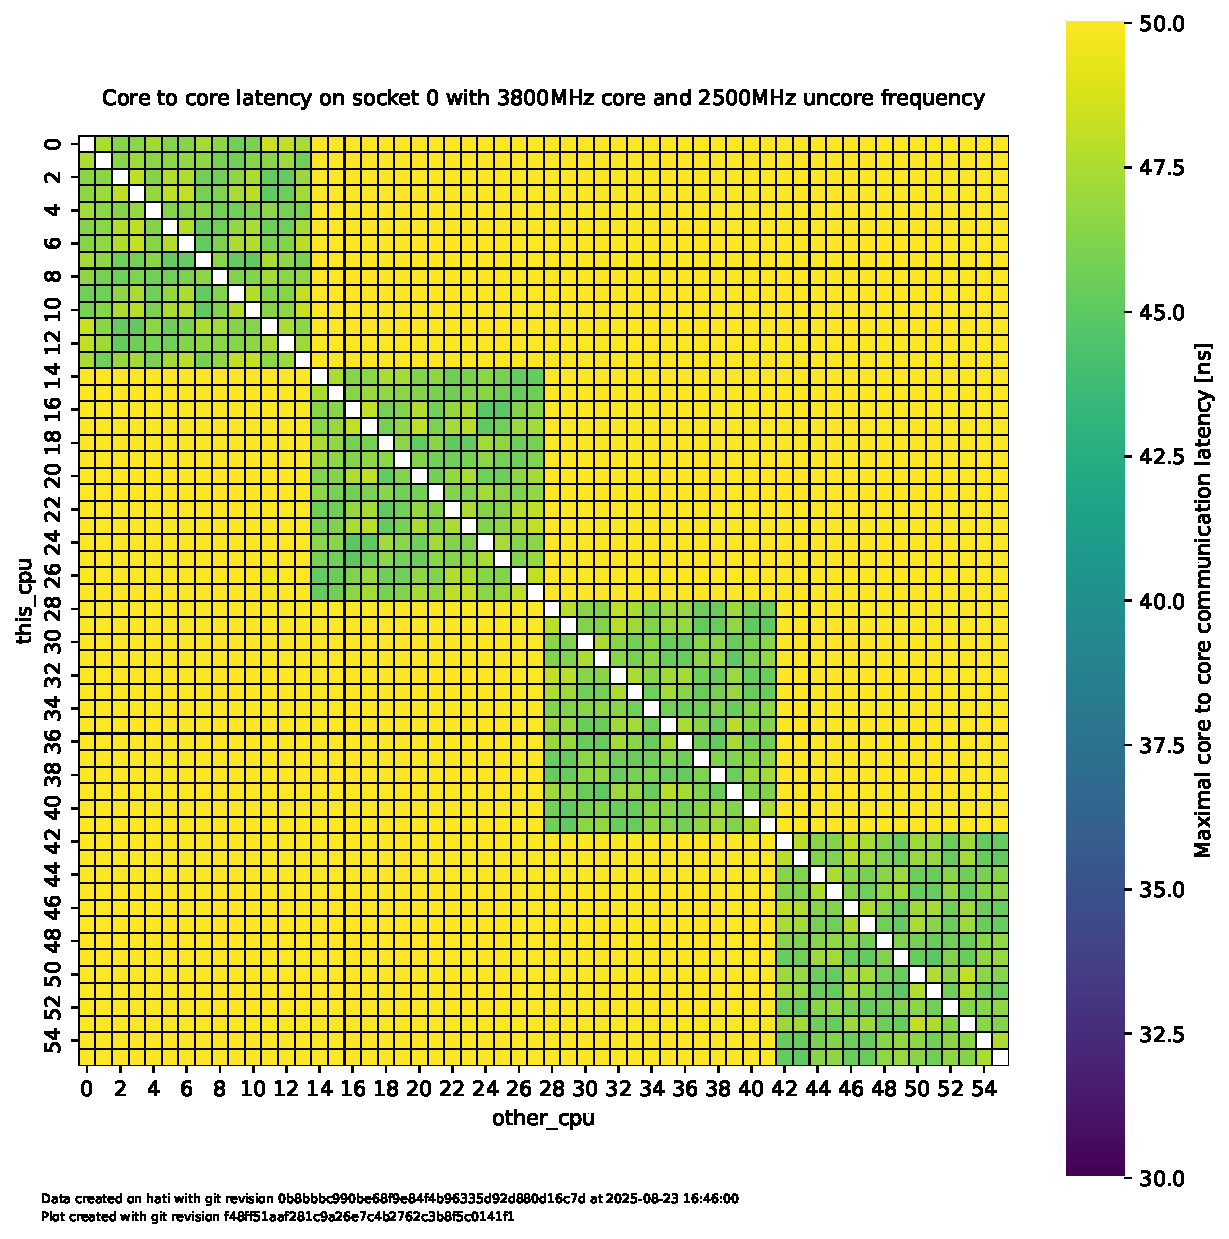
\includegraphics[width=\columnwidth]{fig/core-to-core-latency/core-to-core-heatmap-max-3800-2500.pdf}
    \caption{Maximimal core to core communication latency for hati's socket 0 with \SI{3.8}{\GHz} core and \SI{2.5}{\GHz} uncore frequency.}
\end{figure}
\begin{figure}[]
    \centering
    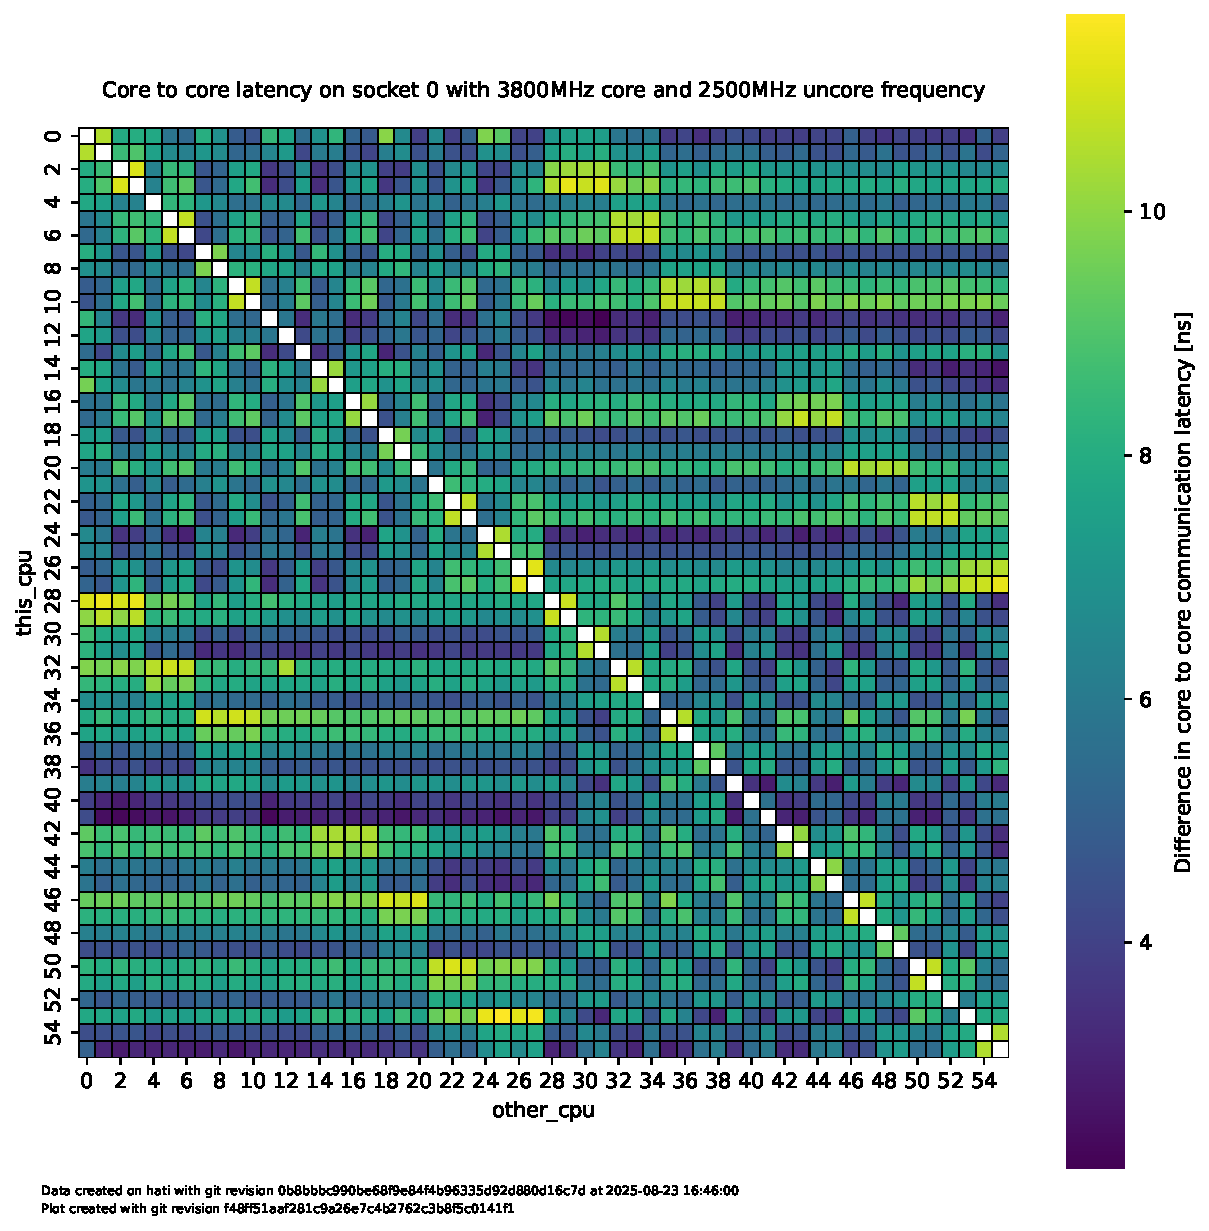
\includegraphics[width=\columnwidth]{fig/core-to-core-latency/core-to-core-heatmap-diff-3800-2500.pdf}
    \caption{Difference in core to core communication latency for hati's socket 0 with \SI{3.8}{\GHz} core and \SI{2.5}{\GHz} uncore frequency.}
\end{figure}